%% abtex2-modelo-trabalho-academico.tex, v-1.9.3 laurocesar
%% Copyright 2012-2015 by abnTeX2 group at http://abntex2.googlecode.com/ 
%% This work may be distributed and/or modified under the
%% conditions of the LaTeX Project Public License, either version 1.3
%% of this license or (at your option) any later version.
%% The latest version of this license is in
%%   http://www.latex-project.org/lppl.txt
%% and version 1.3 or later is part of all distributions of LaTeX
%% version 2005/12/01 or later.
%%
%% This work has the LPPL maintenance status `maintained'.
%% 
%% The Current Maintainer of this work is the abnTeX2 team, led
%% by Lauro César Araujo. Further information are available on 
%% http://abntex2.googlecode.com/
%%
%% This work consists of the files abntex2-modelo-trabalho-academico.tex,
%% abntex2-modelo-include-comandos and abntex2-modelo-references.bib
%%

% ------------------------------------------------------------------------
% ------------------------------------------------------------------------
% abnTeX2: Modelo de Trabalho Academico (tese de doutorado, dissertacao de
% mestrado e trabalhos monograficos em geral) em conformidade com 
% ABNT NBR 14724:2011: Informacao e documentacao - Trabalhos academicos -
% Apresentacao
% ------------------------------------------------------------------------
% ------------------------------------------------------------------------

\documentclass[
	% -- opções da classe memoir --
	12pt,				% tamanho da fonte
	openright,			% capítulos começam em pág ímpar (insere página vazia caso preciso)
	twoside,			% para impressão em verso e anverso. Oposto a oneside
	a4paper,			% tamanho do papel. 
	% -- opções da classe abntex2 --
	%chapter=TITLE,		% títulos de capítulos convertidos em letras maiúsculas
	%section=TITLE,		% títulos de seções convertidos em letras maiúsculas
	%subsection=TITLE,	% títulos de subseções convertidos em letras maiúsculas
	%subsubsection=TITLE,% títulos de subsubseções convertidos em letras maiúsculas
	% -- opções do pacote babel --
	english,			% idioma adicional para hifenização
	brazil				% o último idioma é o principal do documento
	]{abntex2}

% ---
% Pacotes básicos 
% ---
\usepackage{lastpage}			% Usado pela Ficha catalográfica
\usepackage{indentfirst}		% Indenta o primeiro parágrafo de cada seção.
\usepackage{color}				% Controle das cores
\usepackage{graphicx}			% Inclusão de gráficos
\usepackage{microtype} 	
% pacotes adicionados
\usepackage{amsmath}
\usepackage{amssymb,amsfonts,amsthm}
\usepackage{setspace}
\usepackage{float}
\usepackage{listings}
\usepackage{xcolor} % Opcional, para adicionar cores ao código
% ---
		
% ---
% Pacotes adicionais, usados apenas no âmbito do Modelo Canônico do abnteX2
% ---
\usepackage{lipsum}				% para geração de dummy text
% ---
\setlength {\marginparwidth }{2cm}
\usepackage{todonotes}
% ---
% Pacotes de citações
% ---
\usepackage[brazilian,hyperpageref]{backref}	 % Paginas com as citações na bibl
\usepackage[alf]{abntex2cite}	% Citações padrão ABNT
\usepackage{subfig}
\usepackage{subcaption}



\renewcommand{\bf}[1]{\mathbf{#1}}
\renewcommand{\rm}[1]{\mathrm{#1}}


\usepackage{cite}

\lstset{
  language=Matlab,
  basicstyle=\ttfamily\small,      % Estilo da fonte do código
  backgroundcolor=\color{lightgray}, % Fundo cinza claro
  keywordstyle=\color{blue},        % Cor das palavras-chave
  commentstyle=\color{green},       % Cor dos comentários
  stringstyle=\color{red},          % Cor das strings
  numbers=left,                     % Números à esquerda
  numberstyle=\tiny,                % Tamanho dos números
  stepnumber=1,                     % Intervalo entre os números de linha
  numbersep=10pt,                   % Espaçamento entre números e código
  showstringspaces=false,           % Não mostrar espaços nas strings
  breaklines=true,                  % Quebrar linhas longas
  frame=single,                     % Moldura ao redor do código
  captionpos=b,                     % Legenda abaixo do código
}
%\renewcommand\citeleft{[}
%\renewcommand\citeright{]}

% --- 
% CONFIGURAÇÕES DE PACOTES
% --- 
\renewcommand{\imprimircapa}
%\include{modelocapa}}


%\renewcommand{\imprimirfolhaderosto}
%\include{folhaderosto}}


% ---
% Configurações do pacote backref
% Usado sem a opção hyperpageref de backref
\renewcommand{\backrefpagesname}{Citado na(s) página(s):~}
% Texto padrão antes do número das páginas
\renewcommand{\backref}{}
% Define os textos da citação
\renewcommand*{\backrefalt}[4]{
	\ifcase #1 %
		Nenhuma citação no texto.%
	\or
		Citado na página #2.%
	\else
		Citado #1 vezes nas páginas #2.%
	\fi}%
% ---


% ---
% Configurações de aparência do PDF final

% alterando o aspecto da cor azul
\definecolor{blue}{RGB}{41,5,195}

% informações do PDF
\makeatletter
\hypersetup{
     	%pagebackref=true,
		colorlinks=true,       		% false: boxed links; true: colored links
    	linkcolor=blue,          	% color of internal links
    	citecolor=black,        		% color of links to bibliography
    	filecolor=magenta,      		% color of file links
		urlcolor=blue,
		bookmarksdepth=4
}



\makeatother
% --- 

% --- 
% Espaçamentos entre linhas e parágrafos 
% --- 

% O tamanho do parágrafo é dado por:
\setlength{\parindent}{1.3cm}

% Controle do espaçamento entre um parágrafo e outro:
\setlength{\parskip}{0.2cm}  % tente também \onelineskip

% ---
% compila o indice
% ---
\makeindex
% ---

% ----
% Início do documento
% ----
\begin{document}
\graphicspath{ {./images/} }


% Seleciona o idioma do documento (conforme pacotes do babel)
%\selectlanguage{english}
\selectlanguage{brazil}

% Retira espaço extra obsoleto entre as frases.
\frenchspacing 

% ----------------------------------------------------------
% ELEMENTOS PRÉ-TEXTUAIS
% ----------------------------------------------------------
\pretextual

% ---
% Capa
% ---
\imprimircapa
% ---
% Informações de dados para CAPA e FOLHA DE ROSTO
% ---

\titulo{Análise Dinâmica e de Controle do Mini Drone Parrot Mambo Utilizando Matlab Simulink}
\autor{Antonio Cesar Urbano da Silva Filho}
\local{São Bernardo do Campo - SP}
\data{2024}
\orientador{Diego Paolo Ferruzzo Correa}
\instituicao{%
  Universidade Federal do ABC
  \par
  Centro de Modelagem, Engenharia e Ciências Sociais Aplicadas
  }
\tipotrabalho{Trabalho de Gradduação II}
% O preambulo deve conter o tipo do trabalho, o objetivo, 
% o nome da instituição e a área de concentração 
\preambulo{Trabalho elaborado na disciplina Trabalho de Graduação II apresentado ao Centro de Engenharia, Modelagem e Ciências Sociais Aplicadas da Universidade Federal do ABC, no curso de Engenharia Aeroespacial. }
% ---

% ---

% ---
% Folha de rosto
% (o * indica que haverá a ficha bibliográfica)
% ---
\imprimirfolhaderosto
%\include{ficha}
%\include{errata}
%\include{folhaaprova}
%\include{dedicatoria}
%\include{agradecimentos}
%\include{epigrafe}
%\include{resumos}
% ---
% inserir lista de ilustrações
% ---
%\pdfbookmark[0]{\listfigurename}{lof}
%\listoffigures*
%\cleardoublepage
%% ---

% ---
% inserir lista de tabelas
% ---
%\pdfbookmark[0]{\listtablename}{lot}
%\listoftables*
%\cleardoublepage
% ---
%\include{siglas}
% ---
% inserir o sumario
%% ---
%\pdfbookmark[0]{\contentsname}{asd}
%\tableofcontents*
\cleardoublepage
%% ---
\tableofcontents


% ----------------------------------------------------------
% ELEMENTOS TEXTUAIS
% ----------------------------------------------------------
\textual

%\input{Introducão.tex}

%\chapter{\textit{Modelagem dinâmica}}

\section{Modelagem do quadrirrotor}
Um quadricóptero é um tipo de veículo aéreo não tripulado(VANT), caracterizado por ter quatro rotores, que podem ser dispostos em diversas configurações. O Parrot Mambo, utilizado nesse trabalho, dispõe de uma configuração em X, sendo que cada rotor pode variar sua velocidade e direção de giro de maneira independente.

Para estudar as características dinâmicas e o sistema de controle do quadrirrotor deste trabalho, é necessário entender como as forças que interagem com o corpo se relacionam. A análise dinâmica de um drone pode ser dividida na dinâmica de corpo rígido, dinâmica translacional, cinemática e dinâmica de atitude, forças agindo sobre o corpo e controle. Neste capítulo, será apresentada essa análise.

\section{Configurações do quadricóptero}
O Parrot Mambo é um quadricóptero, consistindo de 4 atuadores (conjunto motor e hélice), que são controlados individualmente para gerar empuxo. Dois dos motores giram no sentido horário e dois no anti-horário para que o momento resultante em torno do centro de massa seja zero, prevenindo movimentos indesejados.

O quadricóptero deste estudo tem uma configuração em 'X', que apresenta desempenho de controle superior em rolagem e arfagem (aproximadamente 30\% de vantagem) em relação à configuração em '+', pois utiliza os 4 motores para esses movimentos (Niemiec e Gandhi, 2014). Independentemente da configuração, o quadricóptero tem 6 graus de liberdade, divididos em três para movimento de translação nos eixos \( X \), \( Y \), \( Z \) e três para movimento de rotação em \( \phi \) (rolagem), \( \theta \) (arfagem) e \( \psi \) (guinada).

No entanto, o quadricóptero é sub-atuado, pois tem apenas 4 atuadores. Isso significa que ele não pode controlar diretamente todos os seus movimentos, como deslocar-se lateralmente sem antes rotacionar na direção desejada. Para superar essa limitação, ele combina rotações e empuxo.

\section{Sistemas de coordenadas}
Para a modelagem dinâmica de um quadricóptero, consideramos o sistema de coordenadas inercial $\boldsymbol{\vec{I}}$ = [$\boldsymbol{\vec{X}}$, $\boldsymbol{\vec{Y}}$, $\boldsymbol{\vec{Z}}$], fixo no espaço, e o sistema de coordenadas local $\boldsymbol{\vec{B}}$ = [$\boldsymbol{\vec{X_L}}$, $\boldsymbol{\vec{Y_L}}$, $\boldsymbol{\vec{Z_L}}$], que se move com o quadricóptero.

\begin{figure}[H]
	\centering
	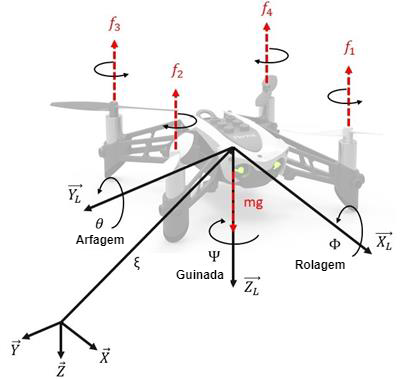
\includegraphics[width=0.6\textwidth]{coordinate-system.png}
	\caption{Representação do sistema de referência inercial e do sistema centralizado no corpo do drone. Fonte: Adaptado de Zaraza Espinosa e Buitrago Galvan (2023).}
	\centering
	\label{fig:coordinate-system}
\end{figure}

\section{Matrizes de rotação}
Agora que os sistemas de referência estão definidos, é necessário relacionar o sistema de referência inercial ($\boldsymbol{\vec{I}}$) com o sistema de referência do corpo ($\boldsymbol{\vec{B}}$) por meio da matriz de rotação $R_{bi}$. Essa matriz é obtida através de três rotações sucessivas ao longo dos eixos do sistema inercial (sequência x-y-z), conforme ilustrado a seguir:

\begin{equation}
	R_{bi}(\phi,\theta,\psi) = R_z(\psi) R_y(\theta) R_x(\phi) =
	\begin{bmatrix}
		cos_\theta cos_\psi & sin_\phi sin_\theta cos_\psi - cos_\phi sin_\psi & cos_\phi sin_\theta cos_\psi + sin_\phi sin_\psi \\
		cos_\theta sin_\psi & sin_\phi sin_\theta sin_\psi + cos_\phi cos_\psi & cos_\phi sin_\theta sin_\psi - sin_\phi cos_\psi \\
		-sin_\theta         & sin_\phi cos_\theta                              & cos_\phi cos_\theta
	\end{bmatrix}
\end{equation}

---

\section{Movimentos do Quadricóptero}
Agora que as características do quadricóptero e as suas configurações foram discutidas, vamos descrever os movimentos que ele pode realizar, associados aos seus 6 graus de liberdade. Cada movimento está relacionado a uma combinação de empuxo gerado pelos atuadores e rotações controladas para superar as limitações do sistema sub-atuado.

\section{Movimento de Rolagem (Roll - $\phi$)}
A rotação em torno do eixo longitudinal ($X$) do quadricóptero, chamada de rolagem, ocorre quando os motores de um lado geram mais empuxo que os motores do lado oposto, inclinando o quadricóptero lateralmente.

\begin{figure}[H]
	\centering
	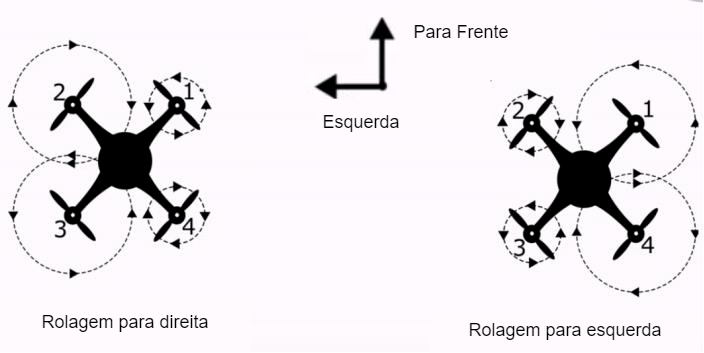
\includegraphics[width=0.8\textwidth]{rolagem-motores.png}
	\caption{Movimento de Rolagem em um quadricóptero com configuração em "X" (Ceppi, 2020).}
	\label{fig:roll_maneuver}
\end{figure}

\begin{figure}[H]
	\centering
	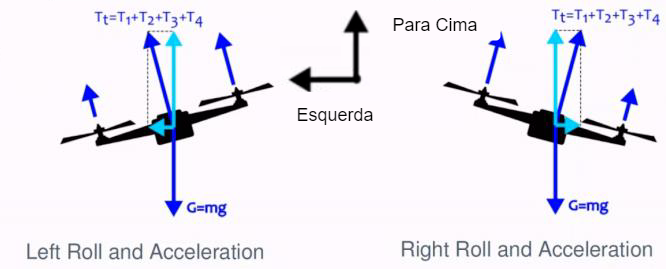
\includegraphics[width=0.8\textwidth]{rolagem-movimento.png} % Substitua por seu caminho de imagem
	\caption{Balanço das forças durante a manobra de Rolagem (Ceppi, 2020).}
	\label{fig:roll_maneuver_forces}
\end{figure}



\section{Movimento de Arfagem (Pitch - $\theta$)}
A arfagem corresponde à rotação em torno do eixo lateral ($Y$), inclinando o quadricóptero para frente ou para trás. Esse movimento resulta do diferencial de empuxo entre os motores dianteiros e traseiros.

\begin{figure}[H]
	\centering
	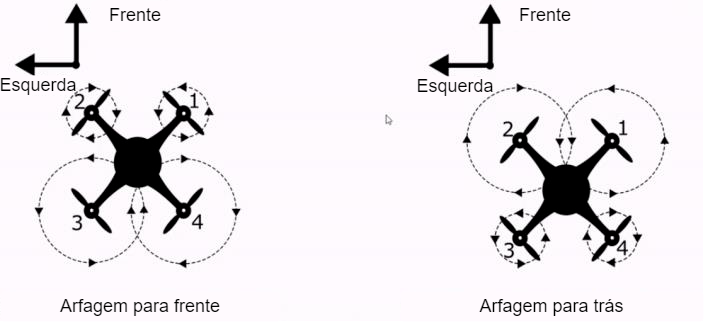
\includegraphics[width=0.8\textwidth]{arfagem-motores.png}
	\caption{Movimento de Arfagem em um quadricóptero com configuração em "X" (Ceppi, 2020).}
	\label{fig:pitch_maneuver}
\end{figure}

\begin{figure}[H]
	\centering
	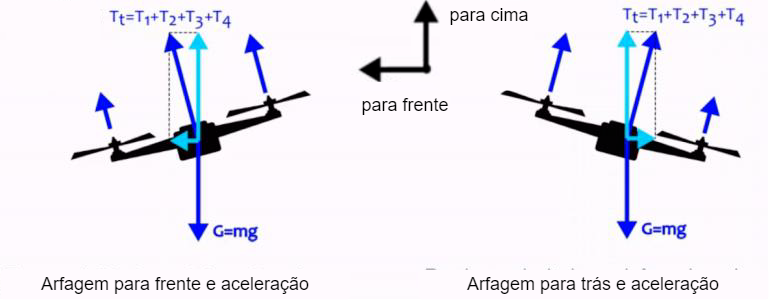
\includegraphics[width=0.8\textwidth]{arfagem-movimento.png} % Substitua por seu caminho de imagem
	\caption{Balanço das forças durante a manobra de Arfagem (Ceppi, 2020).}
	\label{fig:pitch_maneuver_forces}
\end{figure}



\section{Movimento de Guinada (Yaw - $\psi$)}
A guinada refere-se à rotação em torno do eixo vertical ($Z$), que altera a direção do quadricóptero. Isso é conseguido ao variar as rotações dos motores no sentido horário e anti-horário, criando um momento resultante que gira o quadricóptero.

\begin{figure}[H]
	\centering
	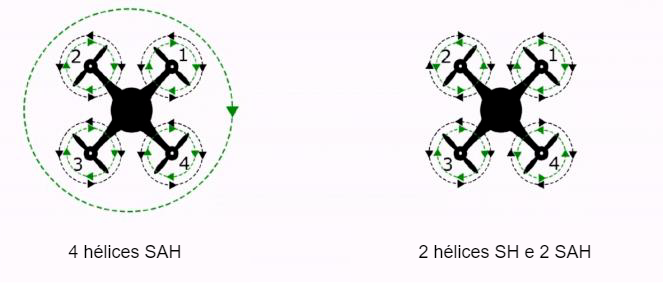
\includegraphics[width=0.8\textwidth]{guinada-motores-movimento.png}
	\caption{Balanço dos torques (Ceppi, 2020).}
	\label{fig:yaw_torques}
\end{figure}


\begin{figure}[H]
	\centering
	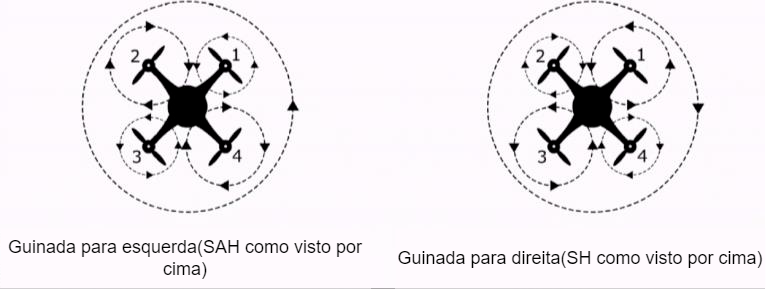
\includegraphics[width=0.8\textwidth]{guinada-movimento.png} % Substitua por seu caminho de imagem
	\caption{Manobra de Guinada e balanço dos torques (Ceppi, 2020).}
	\label{fig:yaw_maneuver_torques}
\end{figure}

\section{Forças e Momentos}

A rotação das hélices gerada pelos motores produz forças de sustentação (empuxo) e momentos sobre o quadricóptero. Essas forças e momentos são fundamentais para o controle e a estabilidade do voo. Nesta seção, detalharemos como essas forças e momentos são calculados e como influenciam a dinâmica do quadricóptero.

\section{Forças Geradas pelas Hélices}

O empuxo produzido por cada hélice é resultado direto da rotação imposta pelo motor. A força de empuxo \( F_i \) gerada pela \( i \)-ésima hélice pode ser expressa pela seguinte equação:

\begin{equation}
F_i = \frac{1}{2} \rho A C_T r_h^2 \Omega_i^2
\label{eq:forca_empuxo}
\end{equation}

Onde:

- \( \rho \) é a densidade do ar (kg/m³).
- \( A \) é a área varrida pela hélice (m²).
- \( C_T \) é o coeficiente de sustentação da hélice (adimensional).
- \( r_h \) é o raio da hélice (m).
- \( \Omega_i \) é a velocidade angular da \( i \)-ésima hélice (rad/s).

Considerando que a densidade do ar e as características geométricas da hélice são constantes durante o voo em baixas altitudes, podemos simplificar a equação definindo uma constante de força \( K_f \):

\begin{equation}
K_f = \frac{1}{2} \rho A C_T r_h^2
\label{eq:constante_forca}
\end{equation}

Assim, a força de empuxo simplifica para:

\begin{equation}
F_i = K_f \Omega_i^2
\label{eq:forca_empuxo_simplificada}
\end{equation}

Essa relação indica que o empuxo é proporcional ao quadrado da velocidade angular da hélice.

\section{Momentos Gerados pelas Hélices}

Além do empuxo, as hélices geram momentos devido ao torque necessário para mantê-las em rotação. O momento \( M_i \) produzido pela \( i \)-ésima hélice é dado por:

\begin{equation}
M_i = \frac{1}{2} \rho A C_D r_h^2 \Omega_i^2
\label{eq:momento_helice}
\end{equation}

Onde:

- \( C_D \) é o coeficiente de arrasto da hélice (adimensional).

Definimos então uma constante de momento \( K_m \):

\begin{equation}
K_m = \frac{1}{2} \rho A C_D r_h^2
\label{eq:constante_momento}
\end{equation}

O momento produzido pela hélice torna-se:

\begin{equation}
M_i = K_m \Omega_i^2
\label{eq:momento_helice_simplificado}
\end{equation}

\section{Força Resultante no Quadricóptero}

Considerando que as forças de empuxo atuam ao longo do eixo \( z_b \) do referencial do corpo, a força total atuante no quadricóptero é a soma das forças individuais:

\begin{equation}
\mathbf{F}_b = \begin{bmatrix}
0 \\
0 \\
- \sum_{i=1}^{4} F_i
\end{bmatrix}
= \begin{bmatrix}
0 \\
0 \\
- K_f (\Omega_1^2 + \Omega_2^2 + \Omega_3^2 + \Omega_4^2)
\end{bmatrix}
\label{eq:forca_total_quadricoptero}
\end{equation}

Definindo o empuxo total \( T \):

\begin{equation}
T = K_f (\Omega_1^2 + \Omega_2^2 + \Omega_3^2 + \Omega_4^2)
\label{eq:empuxo_total}
\end{equation}

A força resultante simplifica para:

\begin{equation}
\mathbf{F}_b = \begin{bmatrix}
0 \\
0 \\
- T
\end{bmatrix}
\label{eq:forca_resultante_simplificada}
\end{equation}

Essa é a força que atua contra a gravidade, permitindo que o quadricóptero suba, desça ou mantenha altitude.

\section{Cálculo dos Momentos Atuantes}

Os momentos que atuam no quadricóptero são originados por dois fatores principais:

1. **Braço de alavanca das forças de empuxo**: Devido à distância entre as hélices e o centro de massa, o empuxo gera momentos em torno dos eixos \( x \) (rolagem) e \( y \) (arfagem).

2. **Momentos de reação das hélices**: Resultantes do torque aplicado pelos motores para girar as hélices, afetando principalmente o eixo \( z \) (guinada).

Os momentos podem ser calculados da seguinte forma:

- **Momento de Rolagem (\( L \))**:

\begin{equation}
L = l (F_4 - F_2) = K_f l (\Omega_4^2 - \Omega_2^2)
\label{eq:momento_rolagem}
\end{equation}

- **Momento de Arfagem (\( M \))**:

\begin{equation}
M = l (F_1 - F_3) = K_f l (\Omega_1^2 - \Omega_3^2)
\label{eq:momento_arfagem}
\end{equation}

Onde:

- \( l \) é a distância horizontal do centro de massa até cada hélice (m).

- **Momento de Guinada (\( N \))**:

\begin{equation}
N = M_1 - M_2 + M_3 - M_4 = K_m (\Omega_1^2 - \Omega_2^2 + \Omega_3^2 - \Omega_4^2)
\label{eq:momento_guinada}
\end{equation}

Os sinais positivos e negativos refletem o sentido de rotação das hélices e, consequentemente, dos momentos gerados.

\section{Interpretação dos Momentos}

- **Rolagem (\( L \))**: Ocorre quando há diferença de empuxo entre as hélices laterais (hélice 2 e hélice 4). Aumentar a velocidade de uma hélice e diminuir a da oposta provoca uma rotação em torno do eixo \( x \).

- **Arfagem (\( M \))**: Resulta da diferença de empuxo entre as hélices dianteira e traseira (hélice 1 e hélice 3). Isso causa uma rotação em torno do eixo \( y \).

- **Guinada (\( N \))**: É gerada pela diferença nos momentos de reação das hélices. Como as hélices giram em sentidos opostos (para balancear o momento total), variar as velocidades de rotação afeta o momento em torno do eixo \( z \).

\section{Resumo das Variáveis Utilizadas}

- \( \rho \) (kg/m³): Densidade do ar.
- \( A \) (m²): Área varrida pela hélice (\( A = \pi r_h^2 \)).
- \( C_T \): Coeficiente de sustentação da hélice.
- \( C_D \): Coeficiente de arrasto da hélice.
- \( r_h \) (m): Raio da hélice.
- \( \Omega_i \) (rad/s): Velocidade angular da \( i \)-ésima hélice.
- \( K_f \): Constante de força, dependente das características da hélice e do ar.
- \( K_m \): Constante de momento, relacionada ao torque de reação da hélice.
- \( l \) (m): Distância do centro de massa até a hélice.
- \( F_i \) (N): Força de empuxo da \( i \)-ésima hélice.
- \( M_i \) (Nm): Momento de reação da \( i \)-ésima hélice.
- \( T \) (N): Empuxo total gerado pelas quatro hélices.
- \( L, M, N \) (Nm): Momentos resultantes em rolagem, arfagem e guinada, respectivamente.

\section{Controle dos Movimentos}

A partir das equações apresentadas, percebe-se que as variáveis de controle fundamentais são as velocidades angulares das hélices \( \Omega_i \). Ao ajustar \( \Omega_i \), podemos controlar:

- **Empuxo Total (\( T \))**: Controlando igualmente as velocidades de todas as hélices, o quadricóptero sobe ou desce.

- **Rolagem (\( L \))**: Variando diferencialmente \( \Omega_2 \) e \( \Omega_4 \), geramos uma rotação em torno do eixo \( x \).

- **Arfagem (\( M \))**: Ajustando \( \Omega_1 \) e \( \Omega_3 \), controlamos a rotação em torno do eixo \( y \).

- **Guinada (\( N \))**: Alterando as velocidades de hélices que giram em sentidos opostos, controlamos a rotação em torno do eixo \( z \).

Dessa forma, o controle preciso das velocidades das hélices permite ao quadricóptero realizar movimentos complexos de translação e rotação.




\section{Movimentos de Translação}
Os movimentos de translação são alcançados através da combinação das rotações já descritas:

\begin{itemize}
	\item \textbf{Translação no eixo X (lateral):} Consequência da inclinação em rolagem.
	\item \textbf{Translação no eixo Y (longitudinal):} Resulta da inclinação em arfagem.
	\item \textbf{Translação no eixo Z (vertical):} Controlada diretamente pela força de empuxo dos quatro atuadores.
\end{itemize}

Os movimentos de translação e rotação são coordenados pelo sistema de controle do quadricóptero, superando as limitações do sistema sub-atuado ao combinar as rotações com o empuxo. Esse mecanismo será detalhado no algoritmo de mistura dos motores.
\begin{align}
	\text{Motor}_{\text{frente-direita}} &= \text{Cmd}_{\text{empuxo}} + \text{Cmd}_{\text{guinada}} + \text{Cmd}_{\text{arfagem}} + \text{Cmd}_{\text{rolagem}} \\
	\text{Motor}_{\text{frente-esquerda}} &= \text{Cmd}_{\text{empuxo}} - \text{Cmd}_{\text{guinada}} + \text{Cmd}_{\text{arfagem}} - \text{Cmd}_{\text{rolagem}} \\
	\text{Motor}_{\text{trás-direita}} &= \text{Cmd}_{\text{empuxo}} - \text{Cmd}_{\text{guinada}} - \text{Cmd}_{\text{arfagem}} + \text{Cmd}_{\text{rolagem}} \\
	\text{Motor}_{\text{trás-esquerda}} &= \text{Cmd}_{\text{empuxo}} + \text{Cmd}_{\text{guinada}} - \text{Cmd}_{\text{arfagem}} - \text{Cmd}_{\text{rolagem}}
\end{align}

\section{Modelo Dinâmico Completo do Quadricóptero}

Após discutirmos a configuração, os sistemas de coordenadas e os movimentos básicos do quadricóptero, podemos agora avançar para o desenvolvimento do modelo dinâmico do quadricóptero. O objetivo desta seção é descrever as equações que governam tanto a translação quanto a rotação do quadricóptero em relação aos sistemas de coordenadas definidos anteriormente.

\section{Dinâmica Translacional}

A dinâmica translacional do quadricóptero pode ser analisada usando a Segunda Lei de Newton, que afirma que a força resultante sobre um corpo é igual à massa do corpo multiplicada pela aceleração de seu centro de massa. No referencial inercial, as forças atuantes no quadricóptero incluem a tração gerada pelos quatro motores e as forças aerodinâmicas de arrasto. Essas forças, inicialmente definidas no referencial do corpo, precisam ser transformadas para o referencial inercial usando as matrizes de rotação definidas anteriormente. 
A tabela \ref{tab:termos_dinamica_translacional} apresenta a descrição dos termos que serão utilizado nas equações da dinâmica translacional.

\begin{table}[H]
	\centering
	\begin{tabular}{|c|l|}
		\hline
		\textbf{Símbolo}  & \textbf{Descrição} \\ \hline
		$m$               & Massa total do quadricóptero \\ \hline
		$x_i, y_i, z_i$   & Coordenadas do centro de massa no referencial inercial \\ \hline
		$\ddot{x_i}, \ddot{y_i}, \ddot{z_i}$ & Acelerações do quadricóptero nas direções \(x_i\), \(y_i\) e \(z_i\) \\ \hline
		$T_i$             & Empuxo gerado pelo \(i\)-ésimo motor \\ \hline
		$\sum_{i=1}^{4} T_i$ & Empuxo total gerado pelos quatro motores \\ \hline
		$\theta$          & Ângulo de arfagem (pitch) \\ \hline
		$\phi$            & Ângulo de rolagem (roll) \\ \hline
		$g$               & Aceleração da gravidade \\ \hline
		$\sin, \cos$      & Funções trigonométricas dos ângulos de rotação \\ \hline
		$R_{ib}$          & Matriz de rotação que transforma do referencial do corpo para o referencial inercial \\ \hline
	\end{tabular}
	\caption{Descrição dos termos utilizados nas equações da dinâmica translacional}
	\label{tab:termos_dinamica_translacional}
\end{table}

Aplicando a Segunda Lei de Newton, pode-se expressar a equação do movimento translacional da seguinte forma:

\begin{equation}
m \begin{bmatrix}
\ddot{x_i} \\
\ddot{y_i} \\
\ddot{z_i}
\end{bmatrix} = R_{ib}
\begin{bmatrix}
0 \\
0 \\
\sum_{i=1}^{4} T_i
\end{bmatrix} - R_{ib}
\begin{bmatrix}
D_x \\
D_y \\
D_z
\end{bmatrix} - m
\begin{bmatrix}
0 \\
0 \\
g
\end{bmatrix}
\end{equation}

Na equação, o primeiro termo no lado direito representa a força de empuxo gerada pelos motores, transformada para o referencial inercial. O segundo termo corresponde à força de arrasto aerodinâmico, que também é transformada para o referencial inercial. O último termo é a força da gravidade, atuando sempre na direção $z_i$ no referencial inercial. Embora o arrasto aerodinâmico seja uma força externa relevante em voos de alta velocidade ou manobras bruscas, optamos por desconsiderá-lo neste modelo, visto que o Parrot Mambo, um quadricóptero de pequeno porte, opera em velocidades relativamente baixas, onde o impacto do arrasto sobre a dinâmica translacional pode ser considerado desprezível.

Assim, iniciaremos falando da força de empuxo $T_i$, que é aplicada ao longo do eixo $z_b$, do referencial do corpo e precisa ser transformada usando a matriz de rotação $R_ib$, que converte as coordenadas do referencial corpo para o referencial inercial.

A força total de empuxo aplicada ao quadricóptero no referencial do corpo é dada por:

\begin{equation}
\mathbf{T} = \begin{bmatrix}
0 \\
0 \\
\sum_{i=1}^{4} T_i
\end{bmatrix}
\end{equation}

Essa força é transformada para o referencial inercial usando a matriz de rotação $R_{ib}$, de forma que:

\begin{equation}
\mathbf{T} = R_{ib} \begin{bmatrix} 
0 \\
0 \\
\sum_{i=1}^{4} T_i 
\end{bmatrix} = 
\begin{bmatrix} 
-\sin\theta \sum_{i=1}^{4} T_i \\
\sin\phi \cos\theta \sum_{i=1}^{4} T_i \\
\cos\phi \cos\theta \sum_{i=1}^{4} T_i
\end{bmatrix}
\end{equation}

A força da gravidade já atua no referencial inercial e é aplicada ao centro de massa do quadricóptero, então não precisamos transforma-la. Sendo que podemos que podemos expressa-lá da seguinte forma no referencial $z_i$:

\begin{equation}
\mathbf{T} = \begin{bmatrix}
0 \\
0 \\
-g
\end{bmatrix}
\end{equation}

Agora podemos combinar os termos de empuxo e gravidade no referencial inercial:

\begin{equation}
m \frac{d^2}{dt^2} \begin{bmatrix} 
x_i \\ 
y_i \\ 
z_i 
\end{bmatrix}
=
\begin{bmatrix} 
-\sin\theta \sum_{i=1}^{4} T_i \\
\sin\phi \cos\theta \sum_{i=1}^{4} T_i \\
\cos\phi \cos\theta \sum_{i=1}^{4} T_i
\end{bmatrix}
- m \begin{bmatrix}
0 \\
0 \\
g
\end{bmatrix}
\end{equation}

Dessa forma, para facilitar a leitura e deixar em um formato de equações, podemos expandir para as equações individuais em cada eixo, além de reorganizar alguns termos. Assim, as equações ficam:


\begin{equation}
\ddot{x_i} = -\frac{T_t}{m} \sin\theta
\end{equation}

\begin{equation}
\ddot{y_i} = \frac{T_t}{m} \sin\phi \cos\theta
\end{equation}

\begin{equation}
\ddot{z_i} = \frac{T_t}{m} \cos\phi \cos\theta - g
\end{equation}

onde:

- \(T_t\) é o empuxo total gerado pelos quatro motores (\(T_t = \sum_{i=1}^{4} T_i\)).

\section{Dinâmica rotacional}

A dinâmica de rotação em drones explora como os torques aplicados à aeronave influenciam suas taxas de rotação angular. Como afirma Hibbeler (2010, p. 600), "a soma dos momentos de todas as forças externas atuando sobre um sistema de partículas (contido em um corpo rígido) em torno de um ponto fixo \(O\) é igual à taxa de variação do momento angular total do corpo em torno do ponto \(O\)", sendo que o ponto \(O\) é a origem do nosso sistema inercial:

\begin{equation}
\vec{M} = \frac{d\vec{H}}{dt}
\end{equation}

onde \(\vec{M}\) representa a soma total de todos os momentos que afetam a rotação do drone, incluindo contribuições externas, como os torques gerados pelos motores e forças aerodinâmicas, e contribuições internas, como os momentos inerciais resultantes da distribuição de massa. O termo \(\vec{H}\) denota o momento angular, cuja variação está associada à rotação do quadrirotor.

O momento angular total de um quadrirotor pode ser dividido em duas componentes: a primeira relacionada à rotação do corpo principal do drone e a segunda associada à rotação dos motores.

Assim, primeiro pode-se expandir o termo do momento angular, o momento angular \(\vec{H}\) é dado por:

\begin{equation}
	\vec{H} = \mathbf{I} \vec{\omega}
\end{equation}

Onde:
\begin{itemize}
    \item \(\mathbf{I}\) é o tensor de inércia (matriz de inércia) do corpo;
    \item \(\vec{\omega}\) é o vetor de velocidade angular.
\end{itemize}

No caso do quadricóptero, onde se um corpo rígido e simétrico, pode-se considerar que o tensor de inércia é constante, e diagonal. 

\begin{equation}
	\boldsymbol{I} = \begin{pmatrix}
		I_{xx} & 0      & 0      \\
		0      & I_{yy} & 0      \\
		0      & 0      & I_{zz}
	\end{pmatrix}
\end{equation}

Onde \( I_{xx} \), \( I_{yy} \) e \( I_{zz} \) são os momentos de inércia ao longo dos eixos \( X \), \( Y \) e \( Z \) do sistema de coordenadas do corpo. 

Assim temos que:

\begin{equation}
\vec{M} = \frac{d\vec{H}}{dt}
\end{equation}

Mas pelo fato do corpo estar rotacionando, a direção do vetor de velocidade angular \(\vec{\omega}\), muda em direção e magnitude com o tempo e é necessário aplicar a derivada vetorial, o que nos leva a:

\begin{equation}
\frac{d}{dt} (\mathbf{I} \vec{\omega}) = \mathbf{I} \frac{d\vec{\omega}}{dt} + \vec{\omega} \times (\mathbf{I} \vec{\omega})
\end{equation}

Onde, o termo \(\mathbf{I} \frac{d\vec{\omega}}{dt}\) é a contribuição direta da variação da velocidade angular \(\vec{\omega}\) com o tempo, e o segundo termo \(\vec{\omega} \times (\mathbf{I} \vec{\omega})\) surge devido à \textbf{derivada de um vetor rotacional}.

E finalmente, substituindo a derivada de \(\vec{H}\) na equação de movimento rotacional \(\vec{M} = \frac{d\vec{H}}{dt}\), temos:


\begin{equation}
\vec{M} = \mathbf{I} \frac{d\vec{\omega}}{dt} + \vec{\omega} \times (\mathbf{I} \vec{\omega})
\end{equation}

Sendo importante notar que aqui, ainda trata-se das velocidades angulares no sistema do corpo, e nosso interesse é tratar dessas velocidades em termos da taxa de variação dos ângulos de Euler, assim temos a matriz de transformação que relaciona as velocidades angulares no referencial do corpo (\(\omega_x\), \(\omega_y\), \(\omega_z\)) com as derivadas dos ângulos de Euler (\(\dot{\phi}\), \(\dot{\theta}\), \(\dot{\psi}\)) pode ser obtida a partir das equações de rotação que descrevem a orientação de um corpo rígido em relação ao sistema de coordenadas inercial. Como discutido por Goldstein (2002, p. xxx), essa matriz leva em conta as interações entre as rotações em torno dos três eixos principais e suas respectivas taxas de variação:

\begin{equation}
\begin{bmatrix}
\omega_x \\
\omega_y \\
\omega_z
\end{bmatrix}
=
\begin{bmatrix}
1 & 0 & -\sin(\theta) \\
0 & \cos(\phi) & \sin(\phi)\cos(\theta) \\
0 & -\sin(\phi) & \cos(\phi)\cos(\theta)
\end{bmatrix}
\begin{bmatrix}
\dot{\phi} \\
\dot{\theta} \\
\dot{\psi}
\end{bmatrix}
\end{equation}

E derivando essas componentes em relação ao tempo:

\begin{equation}
	\frac{d}{dt}
	\begin{bmatrix}
	\omega_x \\
	\omega_y \\
	\omega_z
	\end{bmatrix}
	=
	\begin{bmatrix}
	\ddot{\phi} \\
	\ddot{\theta} \\
	\ddot{\psi}
	\end{bmatrix}
	\end{equation}

Agora calculando o produto vetorial $\vec{\omega} \times (I \vec{\omega})$:

\begin{equation}
\begin{bmatrix}
\omega_x \\
\omega_y \\
\omega_z
\end{bmatrix}
\times
\begin{bmatrix}
I_{xx} \omega_x \\
I_{yy} \omega_y \\
I_{zz} \omega_z
\end{bmatrix}
=
\begin{bmatrix}
\omega_y I_{zz} \omega_z - \omega_z I_{yy} \omega_y \\
\omega_z I_{xx} \omega_x - \omega_x I_{zz} \omega_z \\
\omega_x I_{yy} \omega_y - \omega_y I_{xx} \omega_x
\end{bmatrix}
\end{equation}

Dado que estamos considerando um drone simétrico, podemos simplificar ainda mais. Para um corpo rígido simétrico como um drone, as velocidades angulares 
$\omega_x$, $\omega_y$, e $\omega_z$ podem ser substituídas por suas expressões em termos das taxas de variação dos ângulos de Euler.

Assim, reorganizando nossa equação principal e fazendo as substituições necessárias, temos os momentos em cada cada eixo, em função das velocidades angulares e acelerações angulares. 

\begin{align}
	M_x &= I_{xx} \ddot{\phi} + (I_{zz} - I_{yy}) \dot{\theta} \dot{\psi} \\
	M_y &= I_{yy} \ddot{\theta} + (I_{xx} - I_{zz}) \dot{\phi} \dot{\psi} \\
	M_z &= I_{zz} \ddot{\psi} + (I_{yy} - I_{xx}) \dot{\phi} \dot{\theta}
\end{align}

Entretanto, o que de fato nos interessa são as acelerações angulares.

\begin{align}
	\ddot{\phi} &= \frac{1}{I_{xx}} \left( M_x - (I_{zz} - I_{yy}) \dot{\theta} \dot{\psi} \right) \\
	\ddot{\theta} &= \frac{1}{I_{yy}} \left( M_y - (I_{xx} - I_{zz}) \dot{\phi} \dot{\psi} \right) \\
	\ddot{\psi} &= \frac{1}{I_{zz}} \left( M_z - (I_{yy} - I_{xx}) \dot{\phi} \dot{\theta} \right)
\end{align}

Logo chegamos, nas 6 equações dinâmicas que governam o movimento de um quadricóptero


\begin{equation}
\ddot{x_i} = -\frac{T_t}{m} \sin\theta
\end{equation}

\begin{equation}
\ddot{y_i} = \frac{T_t}{m} \sin\phi \cos\theta
\end{equation}

\begin{equation}
\ddot{z_i} = \frac{T_t}{m} \cos\phi \cos\theta - g
\end{equation}


\begin{align}
	\ddot{\phi} &= \frac{1}{I_{xx}} \left( M_x - (I_{zz} - I_{yy}) \dot{\theta} \dot{\psi} \right) \\
	\ddot{\theta} &= \frac{1}{I_{yy}} \left( M_y - (I_{xx} - I_{zz}) \dot{\phi} \dot{\psi} \right) \\
	\ddot{\psi} &= \frac{1}{I_{zz}} \left( M_z - (I_{yy} - I_{xx}) \dot{\phi} \dot{\theta} \right)
\end{align}


%\chapter{\textit{Análise de Controle}}

Agora que já definimos o comportamento dinâmico de um quadricóptero, nesse capítulo vamos entender como podemos modelar um sistema de controle que seja efetivo no controle das nossas variáveis de interesse, assim passaremos brevemente sobre a teoria de controle e os passos que devemos seguir para montarmos o sistema de controle do quadricóptero em questão. Sendo assim, como este trabalho tem o intuito de analisar o mini drone Mambo da parrot, vamos partir do príncipio que não podemos fazer nenhuma modificação no modelo físico do drone para melhorar sua performance de controle, por exemplo, não podemos adicionar mais um sensor. Então para montarmos nosso problema de controle, precisamos analisar as características do nossa planta, o mini drone Mambo.

\section{Sistemas de Controle}

Podemos definir um sistema como uma coleção de componentes interagindo entre si, exemplos disso podem ser um carro, um motor, ou até mesmo o corpo humano. Sendo assim um sistema pode ser caracterizado por duas propriedades (adicionar citação):

1. Interrelação entre os componentes contidos no sistema.

2. Limites que separam os os componentes dentro do sistema e os que estão fora dele.

Sobre o item 2, quando falamos dos limites que determinam um sistema, esses limites podem ser reais ou imaginários e mutáveis, podendo ser redefinidos a qualquer momento da análise do sistema,por exemplo dividindo um sistema grande em subsistemas, que podem ser analisados separadamente, ou agrupando dois subsistemas em um único sistema.

Assim, quando lidamos com sistemas, nosso maior interesse é nos efeitos que interações externas ao sistema afetam seu comportamento. Na figura abaixo temos a representação de um sistema, onde definimos as interações externas, como entrada, e o resultado da sua interação com o sistema, de saída. O que chamamos de sáida também pode ser chamado de estado do sistema, e pode ser descrito por suas \textit{variáveis de estado}, que em conjunto com a entrada do sistema nos permite determinar seu estado futuro, o que se encaixa na definicão de um sistema dinâmico. Logo quando tratamos de sistemas dinâmicos queremos especificar as entradas do sistema, que o façam se comportar de alguma maneira específica e obtemos isso atráves do controlador, sendo assim quando falamos que nosso interesse está nos efeitos que as entradas causam no estado do sistema, estamos dizendo que queremos controlar a saída do sistema, gerando uma entrada adequada que faça que o sistema e suas váriaveis de estado se comportarem de determinada maneira de interesse. A relação entre o sistema e o controlador é chamada de sistema de controle.

Podemos ter sistemas de controle com feedback e sistemas de controle sem feedeback, estes são chamados respectivamente se sistema de controle de malha fechada e de malha aberta, se observamos as imagens, podemos ver o porquê, um sistema de controle de malha fechada usa feedback para ajustar a ação de controle com base na diferença entre a saída desejada e a saída real, já um sistema de controle de malha aberta a ação de controle é determinada com base na entrada desejada, sem considerar a saída real do sistema.

Nesses sistemas de controle, sempre temos:
- Um processo a ser controlado,o que podemos chamar de planta,
- A váriavel de controle da planta, que chamamos de entrada,
- A variável a ser controlada pela planta, que chamamos de saída,
- O valor de entrada de referência, que nos diz qual a saída desejada,
- O controlador, que a partir do entrada de referência gera o input necessário para que a planta tenha a saída desejada.

O que difere o sistema de malha fechada para o de dmalha aberta são os seguintes componentes:

- Ponto de junção, onde o sinal de saída medido é subtraído do sinal de referência de entrada para medir o sinal de erro.

- Feedback iterativo, onde o sinal de saída é medido com um sensor e retornado para o ponto de junção.



\begin{figure}[H]
	\centering
	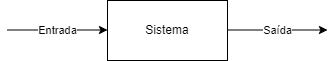
\includegraphics[width=1\textwidth]{controle-sistema-simples.png}
	\caption{Representação de um sistema}
	\centering
	\label{Representação de um sistema}
\end{figure}

\begin{figure}[H]
	\centering
	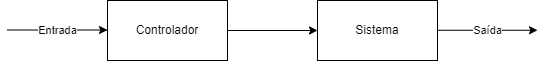
\includegraphics[width=1\textwidth]{controle-sistema-open.png}
	\caption{Representação de um sistema de malha aberta}
	\centering
	\label{Representação de um sistema de malha aberta}
\end{figure}

\begin{figure}[H]
	\centering
	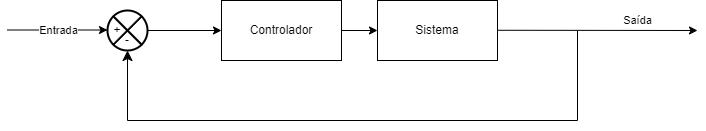
\includegraphics[width=1\textwidth]{controle-sistema-closed.png}
	\caption{Representação de um sistema de malha fechada}
	\centering
	\label{Representação de um sistema de malha fechada}
\end{figure}

\subsection*{Sistema de controle de um quadricóptero}

Na seção anterior, definimos o que é um sistema de controle de forma simples e genérica, com isso em mente agora vamos definir o sistema de controle para um quadricóptero. Nos capítulos anteriores, abordamos as características do quadricóptero que vamos utilizar, sendo assim, conseguimos determinar nosso problema de controle da forma abaixo:

- Planta, que é o modelo dinâmico do nosso quadricóptero;

- Controlador, que é o algoritimo usado para calcular o comando dos motores para que nosso drone atinja o mais precisamente possível a manobra/posição desejada no espaço 3d;

- Sensores, que vão nos ajudar a medir nossas variáveis de estado que serão comparadas com o nosso ponto de referência.


\begin{figure}[H]
	\centering
	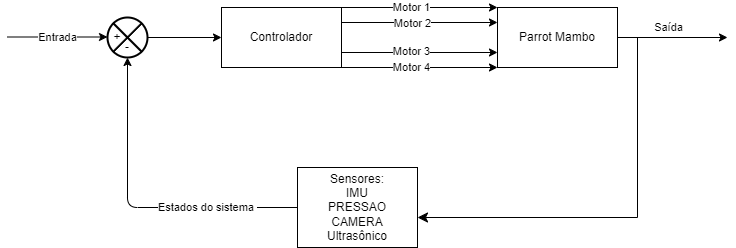
\includegraphics[width=1\textwidth]{controle-sistema-quadricoptero.png}
	\caption{Representação do sistema de controle do Quadricóptero}
	\centering
	\label{Representação do sistema de controle do Quadricóptero}
\end{figure}

Nesse momento nosso foco está no controlador, sendo assim é importante notarmos que esse é um sistema subatuado,pois temos 4 atuadores(motores) e 6 graus de liberdade, o que significa que como nâo temos um atuador para cada movimento nós sabemos que algumas direções não são controladas em momento algum, por exemplo o drone não é capaz de se mover para esquerda sem antes fazer um rolamento, ou para trás e para frente sem antes fazer uma arfagem. Dessa forma, nosso objetivo é superar esse problema do sistema subatuado desenvolvendo um controlador que combina rotações e a propulsão gerada para atingir os objetivos.

Nesse sentido, precisamos saber como gerar propulsão, rolamento, guinada, arfagem com apenas 4 motores e porque a direção de giro das hélices nos permite desacoplar esses movimentos.
A configuração dos drones, geralmente é feita utilizando uma combinação de um par de hélices girando no sentido horário e outro no anti-horário, pois como sabemos, quando as hélices giram, além de produzirem sustentação, elas geram torque na direção oposta de rotação. Assim se todas estivessem girando na mesma direção o drone iria girar incontrolavelmente. Dessa forma podemos controlar esses 4 movimentos de forma independente, da seguinte forma:

- Controle de Propulsão - Todas as hélices girando com a mesma velocidade.

- Controle de Guinada - Para rotacionar o drone em torno do seu eixo vertical, a velocidade de um dos pares de hélices(horário ou anti-horário) tem que ser ajustada. Por exemplo aumentando a velocidade do par de hélices girando no sentido horário e ao mesmo tempo diminuindo a velocidade no sentido anti-horário vai gerar um torque que não vai ser completamente cancelado, fazendo o drone dar uma guinada, enquanto mantém sua altura.

- Controle de Rolamento e Arfagem - Para um rolamento(inclinação para direita ou para esquerda), ou arfagem(inclinação para frente ou para trás). Tem-se que ajudater os pares opostos de hélices. Por exemplo, para uma arfagem para frente, o par de trás aumenta de velocidade e o par da frente diminui a velocidade.

Sendo assim esses são os quatro movimentos que podemos controlar independentemente, e o comando para os motores será uma mistura da propulsão, guinada, rolagem e arfagem necessária.

SA - Sentido horário
SAH - Sentido anti-horário

\begin{table}[h!]
	\centering
	\begin{tabular}{|c|c|c|c|}
	\hline
	{\textbf{Command}} & \multicolumn{3}{c|}{\textbf{Cross Configuration}} \\ \cline{2-4}
	 & \textbf{Estado da Velocidade} & \textbf{PAR 1, 3} & \textbf{PAR 2, 4} \\ \hline
	\textbf{Pairar (H)} & $\omega_{m1} = \omega_{m3}$ & $\omega_{m2} = \omega_{m4}$ & \textbf{PAR 1, 3 = PAR 2, 4} \\ \hline
	\textbf{SH Arfagem} & $\omega_{m1} > \omega_{m3}$ & $\omega_{m2} > \omega_{m4}$ & N/A \\ \hline
	\textbf{SH Rolagem} & $\omega_{m1} < \omega_{m3}$ & $\omega_{m2} > \omega_{m4}$ & N/A \\ \hline
	\textbf{SH Guinada} & $\omega_{m1} = \omega_{m3}$ & $\omega_{m2} = \omega_{m4}$ & \textbf{Par 1, 3} < \textbf{ Par 2, 4} \\ \hline
	\textbf{SAH Arfagem} & $\omega_{m1} < \omega_{m3}$ & $\omega_{m2} < \omega_{m4}$ & N/A \\ \hline
	\textbf{SAH Rolagem} & $\omega_{m1} > \omega_{m3}$ & $\omega_{m2} < \omega_{m4}$ & N/A \\ \hline
	\textbf{SAH Guinada} & $\omega_{m1} = \omega_{m3}$ & $\omega_{m2} = \omega_{m4}$ & \textbf{Par 1, 3} > \textbf{ Par 2, 4}\\ \hline
	\end{tabular}
	\caption{Tabela de Comandos para Configuração Cross}
	\label{tab:control-config}
	\end{table}

	\begin{figure}[h]
		\centering
		\begin{equation*}
			\begin{aligned}
				\text{Motor}_{\text{frontal direito}} & = \text{Propulsão} + \text{Guinada}_{\text{cmd}} + \text{Arfagem}_{\text{cmd}} + \text{Rolagem}_{\text{cmd}} \\
				\text{Motor}_{\text{frontal esquerdo}} & = \text{Propulsão} + \text{Guinada}_{\text{cmd}} + \text{Arfagem}_{\text{cmd}} - \text{Rolagem}_{\text{cmd}} \\
				\text{Motor}_{\text{traseiro direito}} & = \text{Propulsão} + \text{Guinada}_{\text{cmd}} + \text{Arfagem}_{\text{cmd}} + \text{Rolagem}_{\text{cmd}} \\
				\text{Motor}_{\text{traseiro esquerdo}} & = \text{Propulsão} + \text{Guinada}_{\text{cmd}} + \text{Arfagem}_{\text{cmd}} - \text{Rolagem}_{\text{cmd}}
			\end{aligned}
		\end{equation*}
		\caption{Algoritimo dos motores do drone}
	\end{figure}

Como já comentamos, os movimentos para trás, pra frente, para direita e para esquerda, não são atuados, e nos movimentos nessas direções, primeiro rotacionando o drone numa atitude onde nosso vetor de propulsão está parcialmente na direção da gravidade e parcialmente na direção que escolhemos ir, para acelerarmos o drone naquela direção, sendo assim para manter altura durante essa manobra, precisamos aumentar a propulsão de forma que ela continue a cancelar a ação da gravidade.

\subsection*{Controlador de Voo Pairado}

Com o que já vimos nos capítulos anteriores, agora podemos desenvolver nosso controlador. Para isso, vamos utilizar a missão mais simples de voo que é um voo pairado, ou seja, queremos que nosso drone levante voo e não se mova signficativamente no plano X,Y. Assim sendo temos que controlar a posição do drone no plano X,Y,Z, a partir das nossas quatro váriaveis controláveis independentemente, rolagem, guinada, arfagem e propulsão.

A principio para um voo pairado, podemos pensar em um controlador de altitude,  que tem como entrada a altitude, aumentando ou diminuindo a propulsão até atingir a altitude necessária, no formato abaixo:

\begin{figure}[H]
	\centering
	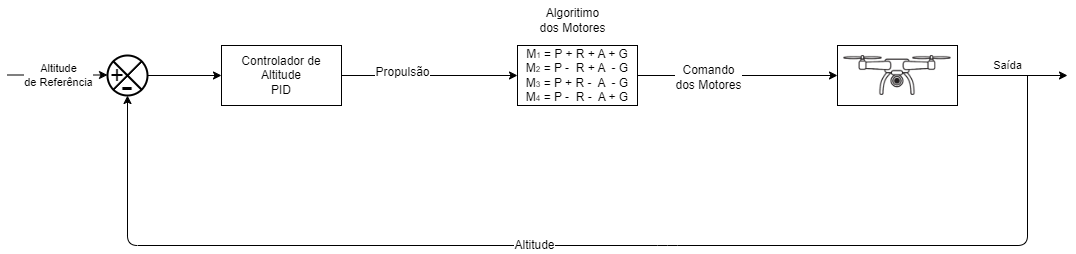
\includegraphics[width=1\textwidth]{flightControlSystem-controller-manbo-altitude.png}
	\caption{Sistema de controle utilizando apenas Propulsão para Controle de Altitude}
	\centering
	\label{Sistema de controle utilizando apenas Propulsão para Controle de Altitude}
\end{figure}


\begin{figure}[H]
	\centering
	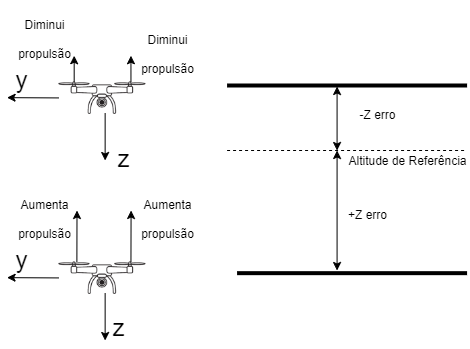
\includegraphics[width=1\textwidth]{flightControlSystem-controller-manbo-altitude-work.png}
	\caption{Funcionamento de um sistema de Controle utilizando apenas Propulsão para Controle de Altitude}
	\centering
	\label{Funcionamento de um sistema de Controle utilizando apenas Propulsão para Controle de Altitude}
\end{figure}

Em mundo ideal, sem nenhuma perturbação, como o vento, considerando que todos os motores estão perfeitamente calibrados,e que o aumento da propulsão vai gerar apenas aumento na velocidade em Z, este seria um ótimo controlador, mas no mundo real essa não é a situação que temos, geralmente temos perturbações naturais como rajadas de vento, ou neve, os motores podem estar descalibrados entre si então um aumento na propulsão pode causar aumento na velocidade horizontal. Ou seja nosso sistema ainda não está preparado para lidar com o mundo real, por exemplo uma rajada de vento pode causar uma mudança no ângulo de rolagem ou arfagem fazendo com que o aumento da propulsão cause aumento na velocidade horizontal do drone o fazendo se movimentar no plano XY descontroladamente, se afastando do ponto de partida, então o drone atingiria a altitude necessária, que é o objetivo, mas se movimentaria no plano XY, que não é o objetivo. Assim, diferente do que pode-se pensar inicialmente, temos que controlar nossas quatro váriaveis independentemente. E teríamos um sistema de controle como o abaixo.


\begin{figure}[H]
	\centering
	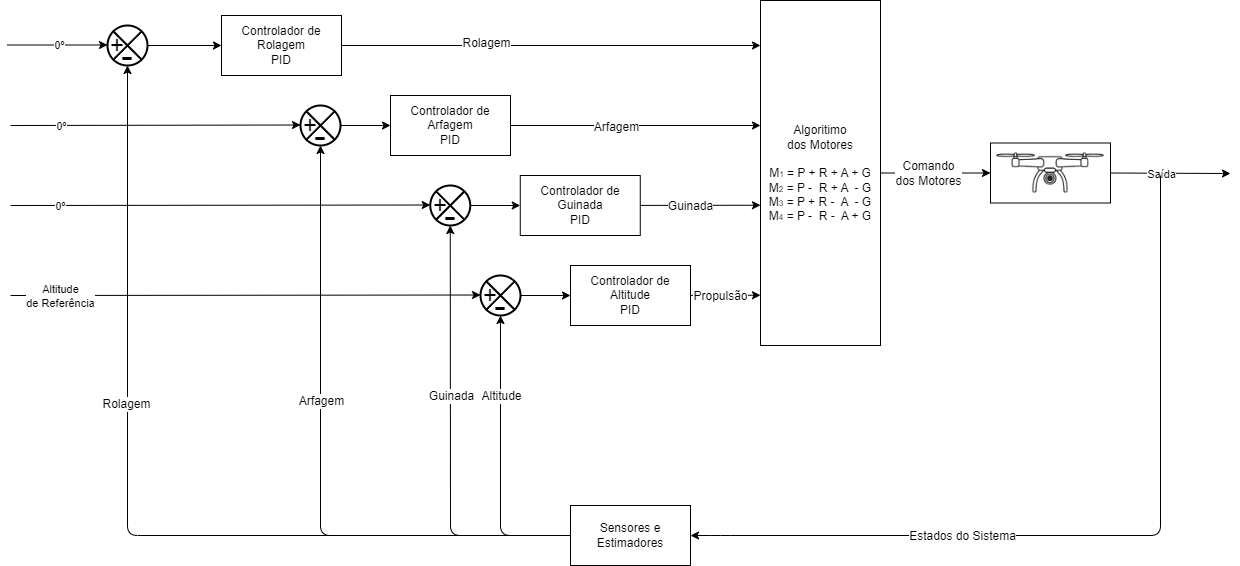
\includegraphics[width=1\textwidth]{flightControlSystem-controller-manbo-4-controllers.png}
	\caption{Sistema de Controle utilizando todas as variáveis controláveis}
	\centering
	\label{Sistema de Controle utilizando todas as variáveis controláveis}
\end{figure}

O que considera todas as nossa variáveis controláveis, mas se observarmos com atenção e fizermos o exercício de considerar uma rajada de vento lateral temos que:


- \( t_0 \) - Drone está fazendo voo pairado (\(\phi = 0\)), (\(\psi = 0\)) e (\(\theta = 0\)), (\(\dot{\phi} = 0\)), (\(\dot{\psi} = 0\)) e (\(\dot{\theta} = 0\)), (\(\dot{x} = 0\)), (\(\dot{y} = 0\)), (\(\dot{z} = 0\)), \( Z > 0 \), \( X = 0 \), \( Y = 0 \);

- \( t_1 \) - Drone recebe rajada de vento (\(\phi = 0\)), (\(\psi = 0\)) e (\(\theta > 0\)), (\(\dot{\phi} = 0\)), (\(\dot{\psi} = 0\)) e (\(\dot{\theta} > 0\)), (\(\dot{x} > 0\)), (\(\dot{y} = 0\)), (\(\dot{z} < 0\)), \( Z > 0 \), \( X > 0 \), \( Y = 0 \).

- \( t_2 \) - Drone ajusta ângulos de guinada, arfagem e rolagem e altitude (\(\phi = 0\)), (\(\psi = 0\)) e (\(\theta = 0\)), (\(\dot{\phi} = 0\)), (\(\dot{\psi} = 0\)) e (\(\dot{\theta} = 0\)), (\(\dot{x} = 0\)), (\(\dot{y} = 0\)), (\(\dot{z} = 0\)), \( Z > 0 \), \( X > 0 \), \( Y = 0 \);

Assim, podemos notar que, apesar de ajustarmos nossas quatro varráveis atuadas e conseguirmos ter um voo pairado. Caso esse ciclo se repetisse, a cada rajada de vento a posição \( X \) iria aumentar devido à aceleração nesse eixo causada pelo breve instante entre a rolagem (\(\theta > 0\)) e a correção do ângulo (\(\theta = 0\)). Ou seja esse sistema de controladores que elaboramos ainda é insuficiente para o nosso objetivo que é realizar um voo pairado e que apesar das perturbações externas faça o voo sem se afastar do local de decolagem.


\begin{figure}[H]
	\centering
	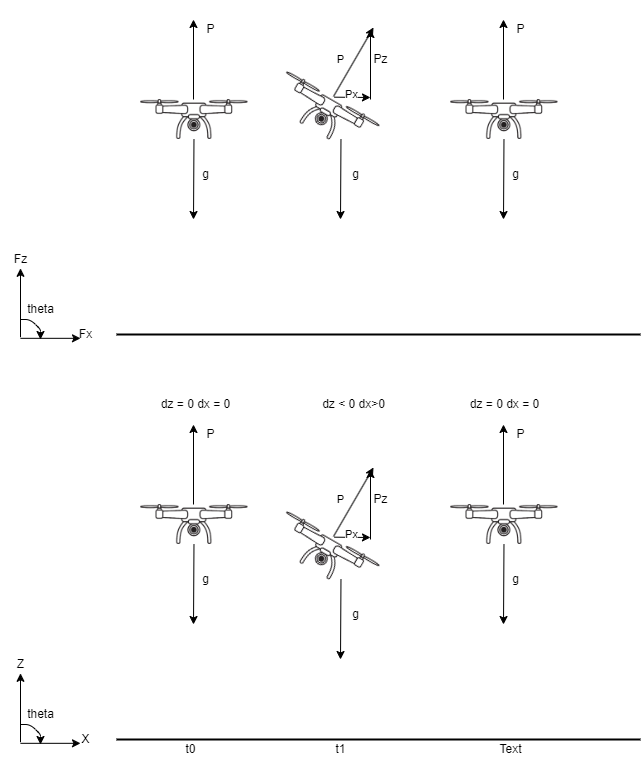
\includegraphics[width=1\textwidth]{flightControlSystem-controller-manbo-altitude-work-wind.png}
	\caption{Drone sobre influência de rajada de vento controlando apenas 4 váriaveis atuadas}
	\centering
	\label{Drone sobre influência de rajada de vento controlando apenas 4 váriaveis atuadas}
\end{figure}

Ou seja, assumir que para um voo pairado nossos ângulos de guinada, arfagem e rolagem tem que ser zero, não é uma boa interpretação para o nosso sistema de controle então, mas também não queremos fixar ângulos específicos de arfagem e rolagem, na verdade nosso objetivo está em controlar a posição em relação ao solo, plano X,Y.

Assim, podemos adicionar um controlador de posição que vai conter controladores de arfagem e rolagem para manter a posição em X,Y. Nesse sentido, os controladores de arfagem e rolagem internos ao controlador de posição vão calcular a entrada de referência para os controladores de arfagem e rolagem. Logo temos o loop externo, que gera os sinais de referência de arfagem e rolagem para o loop interno, sendo importante notar que o ângulo de guinada também vai ser utilizado no controlador de posição. Os erros de posição X-Y são expressos em relação ao referencial do ambiente, mas os ângulos de arfagem e rolagem são expressos em relação ao referencial do drone. Isso significa que um movimento nas direções X e Y do mundo pode ser obtido através da arfagem e rolagem apenas conhecendo o ângulo de guinada, pois ele é necessário para o controlador de posição fazer a conversão do referencial X-Y do drone para o referencial do ambiente.
 

\begin{figure}[H]
	\centering
	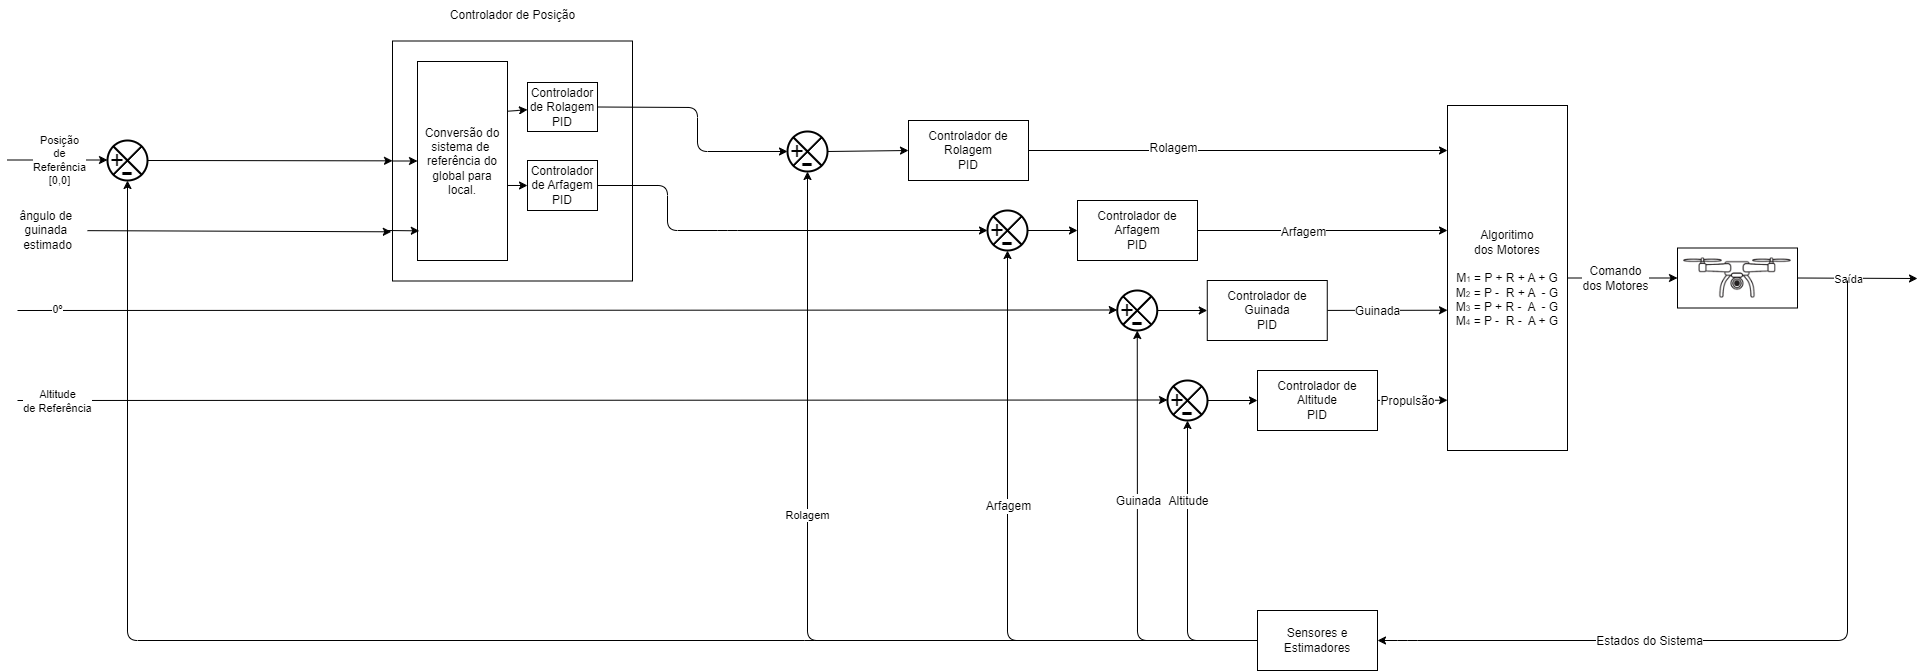
\includegraphics[angle=90,width=0.5\textwidth]{flightControlSystem-controller-manbo-6-controllers-complete.png}
	\caption{Sistema de controle de um quadricóptero para Voo Pairado}
	\centering
	\label{Sistema de controle de um quadricóptero para Voo Pairado}
\end{figure}

Outro ponto importante de notarmos no nosso sistema, é que apesar de termos idealizado ele pensando em um voo pairado, ele pode ser útil para outros objetivos, como por exemplo navegar para uma posição específica e pousar. O que é importante nesse controlador que idealizamos é que podemos controlar os 6 graus de liberdade do drone.

Podemos inclusive lembrar do exercício que fizemos acima, sobre os instantes e teríamos uma mudança em \( t_2 \) e no próximo instante estaríamos na posição original no plano XY.

- \( t_2 \) - Drone ajusta ângulos de guinada, arfagem e rolagem e altitude e posição em x (\(\phi = 0\)), (\(\psi = 0\)) e (\(\theta = 0\)), (\(\dot{\phi} = 0\)), (\(\dot{\psi} = 0\)) e (\(\dot{\theta} < 0\)), (\(\dot{x} > 0\)), (\(\dot{y} = 0\)), (\(\dot{z} = 0\)), \( Z > 0 \), \( X > 0 \), \( Y = 0 \);

- \( t_3 \) - Drone na posição original, pairando sobre o ponto de decolagem (\(\phi = 0\)), (\(\psi = 0\)) e (\(\theta = 0\)), (\(\dot{\phi} = 0\)), (\(\dot{\psi} = 0\)) e (\(\dot{\theta} = 0\)), (\(\dot{x} = 0\)), (\(\dot{y} = 0\)), (\(\dot{z} = 0\)), \( Z > 0 \), \( X = 0 \), \( Y = 0 \);
%---------------------------------------------------------------------
% INDICE REMISSIVO
%---------------------------------------------------------------------
\phantompart
\printindex
%---------------------------------------------------------------------


%\chapter{\textit{Análise dinâmica e Controle Mini Parrot}}

Nos capítulos anteriores construímos uma base teórica sobre dinâmica e controle de um quadricóptero, assim, nesse capítulo vamos relacionar o que foi dito nos capítulos anteriores com o sistema de controle desenvolvido pela MathWorks em parceria com a parrot para fins de estudo. 

O sistema de controle já desenvolvido é bem completo e complexo, então nossa intenção será avaliar as características do sistema de controle durante um voo pairado e verificar a possibilidade de implementar melhorias no sistema.

\section{Características do quadricóptero}

O quadricóptero selecionado foi o Parrot Mambo Fly, esse é um drone pequeno(18 x 18 x 4 cm), e leve (~68 gramas). O quadricóptero utiliza uma configuração de rotores em "X", onde o eixo X do sistema de referência do corpo é alinhado entre os dois rotores frontais, diferente deê um drone com configuração em "+" onde o eixo x aponta diretamente para o rotor frontal. Cada rotor têm um motor de corrente continua sem escovas. Além disso o quadricóptero tem autonomia entre 8 e 10 minutos, a partir de uma bateria de litio de 660mAh. A memória interna do drone é de 1GB, e ele tem um processador com velocidade de 200Hz. O drone também conta com alguns sensores que são utilizados para o controle, são eles:

- Camera: Uma cãmera de 0.3 megapixel, que fica na parte de baixo do drone, com uma taxa de quadros de 60 fps. Utilizada para medir o deslocamento horizontal do drone com o método de fluxo ótico, que consiste em estimar a velocidade baseada no movimento relativo entre os quadros.

- Ultrasom: O sensor ultrasônico, localizado também na parte debaixo do drone, mede a posição vertical do drone relativo ao solo, ou seja, mede a altitude. A faixa de operação desse sensor é de 4 metros. 

- Sensor de Pressão: É utilizado para medir a altitude do drone, quando essa for maior do que 4 metros(faixa de operação do sensor ultrasônico), utilizando-se do fato que a pressão atmosférica é inversamente proporcional a altitude.

- IMU: Composta por um acelerômetro de 3 eixos que mede a aceleração linear e um giroscópio de 3 eixos para medição da velocidade angular.

Como já dissemos o drone tem uma configuração em "X", e é importante notar que os motores opostos rotacionam na mesma direção, mas na direção inversa do outro par. Isso é necessário para que possamos controlar, a propulsão, a rolagem, a guinada e a arfagem de maneira independente(apesar do fato que existe acoplamento entre os movimentos, mas para os nosso propósito vamos desconsiderá-los).

Agora que já temos noção das características do nosso drone, vamos analisar o sistema de controle desenvolvido pela MathWorks para testes e simulações com o Parrot Mambo minidrone.

\section{O projeto do quadricóptero no Matlab Simulink}

Primeiramente para abrir o projeto no matlab, temos que rodar o comando \textit{asbQuadcopterStart}, iniciando assim o projeto. Onde podemos ver todos os componentes que compõe o sistema de controle. 

\begin{figure}[H]
	\centering
	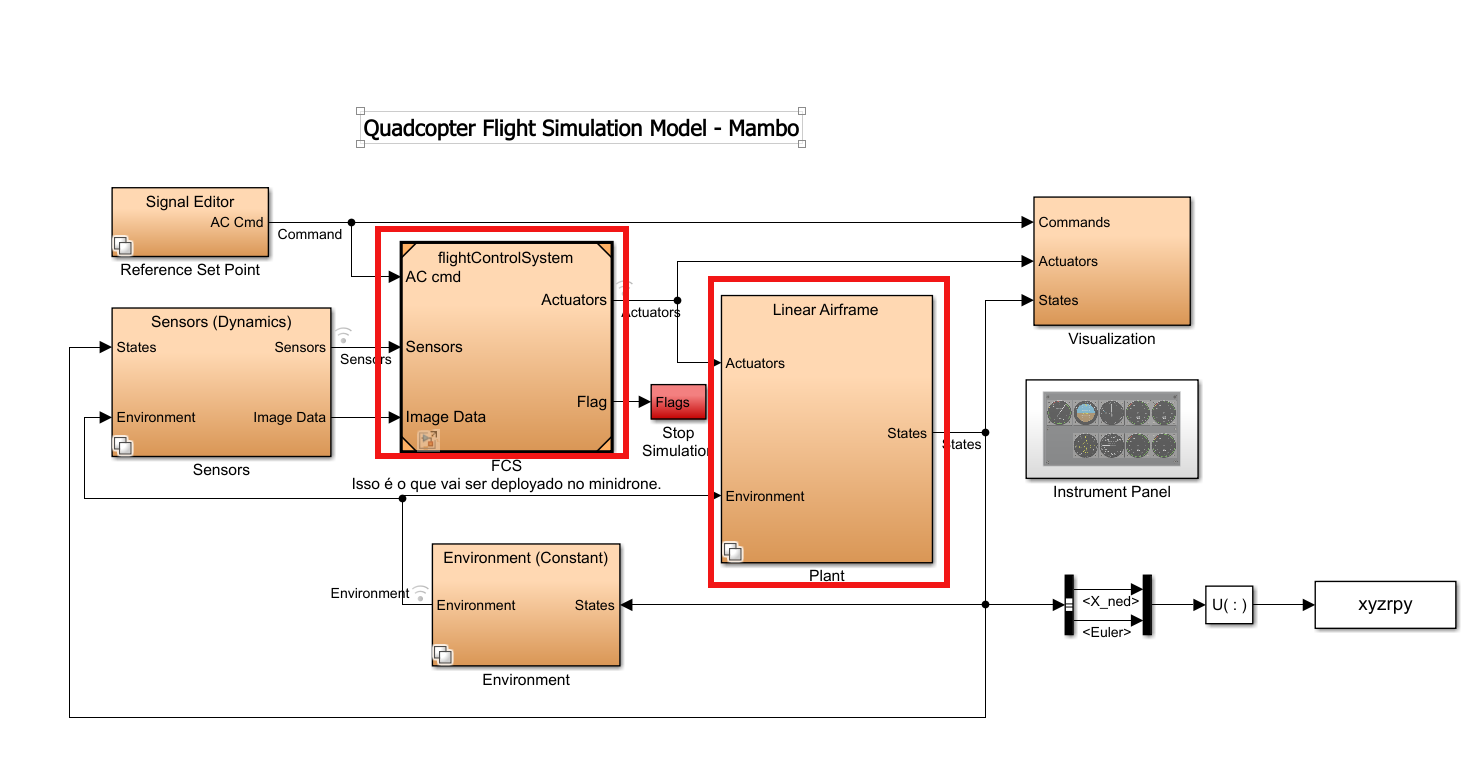
\includegraphics[width=0.6\textwidth]{asbQuadcopterProject}
	\caption{Modelo de Voo do Quadricóptero Parrot Mambo}
	\centering
	\label{Modelo de Voo do Quadricóptero Parrot Mambo}
\end{figure}

Não é o foco desse trabalho analisar todos os componentes desse modelo,analisaremos apenas os componentes em destque na figura, vamos focar no Sistema de Controle de Voo, que é o nosso controlador(recebe as medidas dos sensores e calcula o input para a planta, além disso pode ser implantado no drone), e na planta que é o modelo físico do nosso drone. Entretantom falaremos brevemente sobre os outros componentes.

Reference Set Point - Define qual tipo de entrada será usada como comando, temos 4 opções, joystick(controle remoto), sinais(entradas temporais), dados em função do tempo em um arquivo .mat ou .xlsx.

Sensors - Os sensores que a partir de suas medidas vão calcular o estado atual das nossas variáveis de interesse.

Environment - É uma constante que define se nas simulações será usado um modelo constante de ambiente externo(gravidade constante, pressão constante, etc), ou um modelo dinâmico, onde esses valores variam de acordo com a altura e posição.

Visualization - Construído para para extrair e apresentar os dados de voo e possui 4 formas de visualização, além de extrair os dados necessários para o "Instrument Panel"

Instrument Panel - Painel instrumentado para visualização de alguns dados de voo.

\subsection{Sistema de Controle de Voo}

\begin{figure}[H]
	\centering
	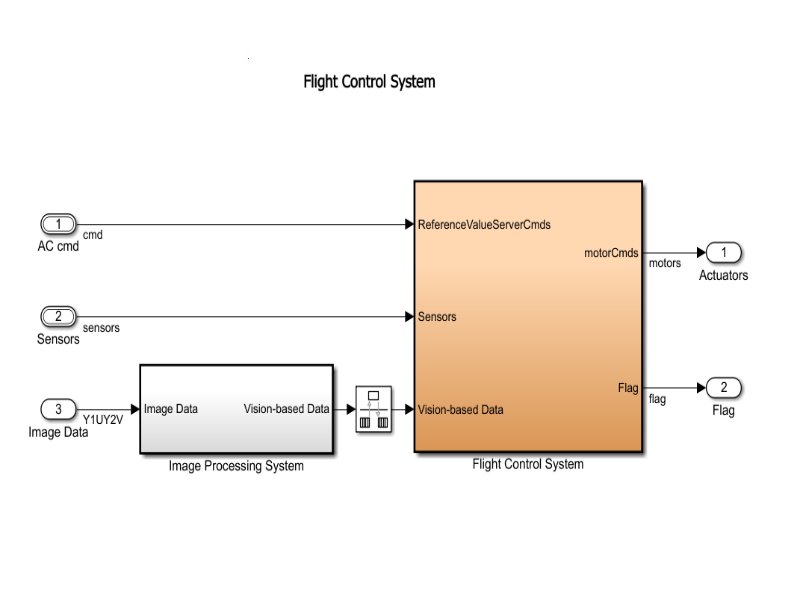
\includegraphics[width=0.6\textwidth]{flightControlSystem}
	\caption{Modelo do sistema de controle de voo}
	\centering
	\label{flightControlSystem}
\end{figure}

Na arquitetura definida pela parrot no simulink, podemos observar que o controlador recebe os valores de referência dos comandos, os dados dos sensores(menos da câmera), e os dados da câmera separadamente. E seus parâmetros de saída são os comandos para os motores atingirem a posição desejada e um parâmetro para prevenção de batidas acidentais. Assim, na sequência vamos adrentar no bloco principal da imagem acima(Flight Control System), e entender seu funcionamento.


\begin{figure}[H]
	\centering
	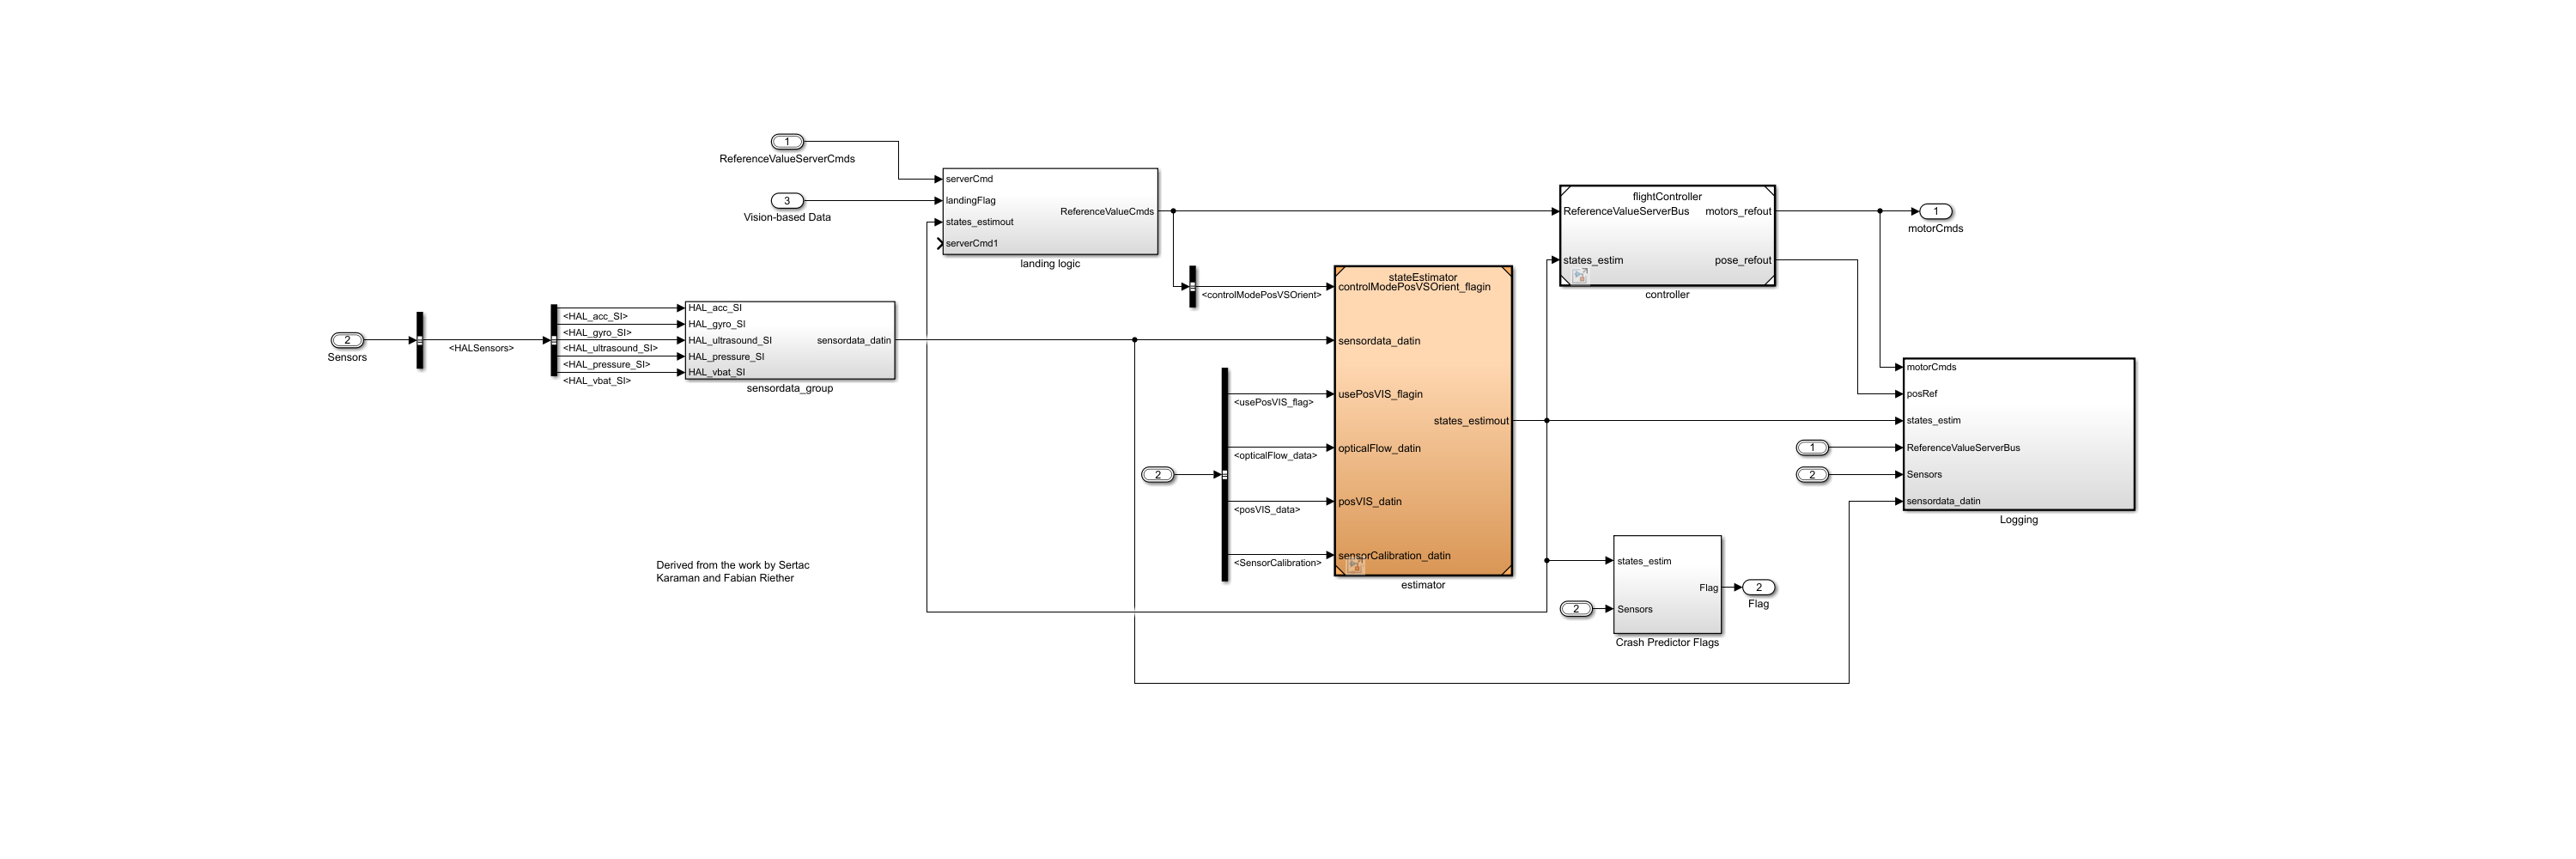
\includegraphics[width=1\textwidth]{flightControlSystem-inside}
	\caption{Dentro do Sistema de controle de Voo}
	\centering
	\label{flightControlSystem-inside}
\end{figure}


Aqui podemos ver alguns blocos importantes:

- Sensor Data Group: Agrup os dados dos sensores de forma mais adequada para ser usada durante o restante do fluxo, como podemos ver na imagem abaixo.

\begin{figure}[H]
	\centering
	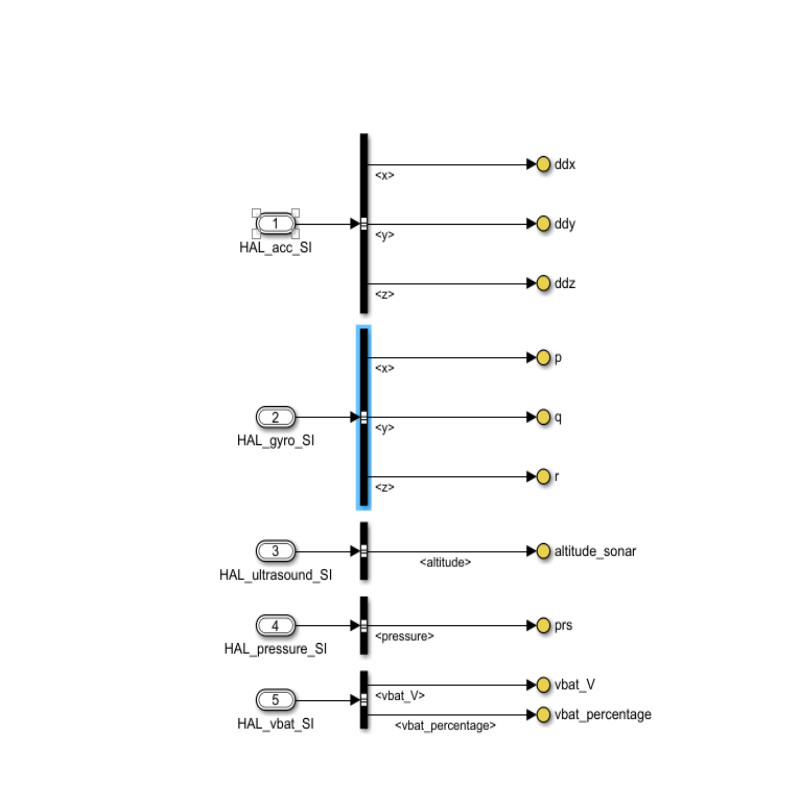
\includegraphics[width=1\textwidth]{flightControlSystem-sensordatagroup}
	\caption{Agrupamento de dados dos sensores}
	\centering
	\label{flightControlSystem-sensordatagroup}
\end{figure}

- Landing Logic - Contém a lógica para um pouso controlado, vamos falar mais sobre ela em breve com o intuito de utiliza-lá para simulações. 

- Estimator - É o estimador de estado do nosso sistema de controle, ele recebe basicamente todos os dados coletados pelos sensores e agrupados a partir do "Sensor Data Group",os dados de calibração desses sensores, além dos dados coletados da câmera a partir da técnica de fluco ótico(optical flow). Com o intuito de estimar o estado completo do quadricóptero, ou seja sua posição X,Y,Z, sua velocidade dx, dy, dz e sua orientação, ângulo rolagem($\phi$), arfagem($\phi$) e guinad($\psi$), e também a orientação do corpo no sistema de referência do corpo.
Olhando dentro do estimador de estados, podemos ver alguns blocos importantes:

-Sensor Pré-Processing: Pré processa os dados dos sensores, e valida alguns dados das câmeras para saber se podem ser utilizados.

-Complementary Filter: Filtro complementar com o intuito de combinar os diferentes sensores e obter medições mais precisas, da orientação do quadricóptero.

-Estimator XY Position: Responsável por estimar as posições XY, além das velocidades nesses eixos. 

-Estimator Altitude: Responsável por estimar a posição no eixo Z e sua respectiva velocidade.

\begin{figure}[H]
	\centering
	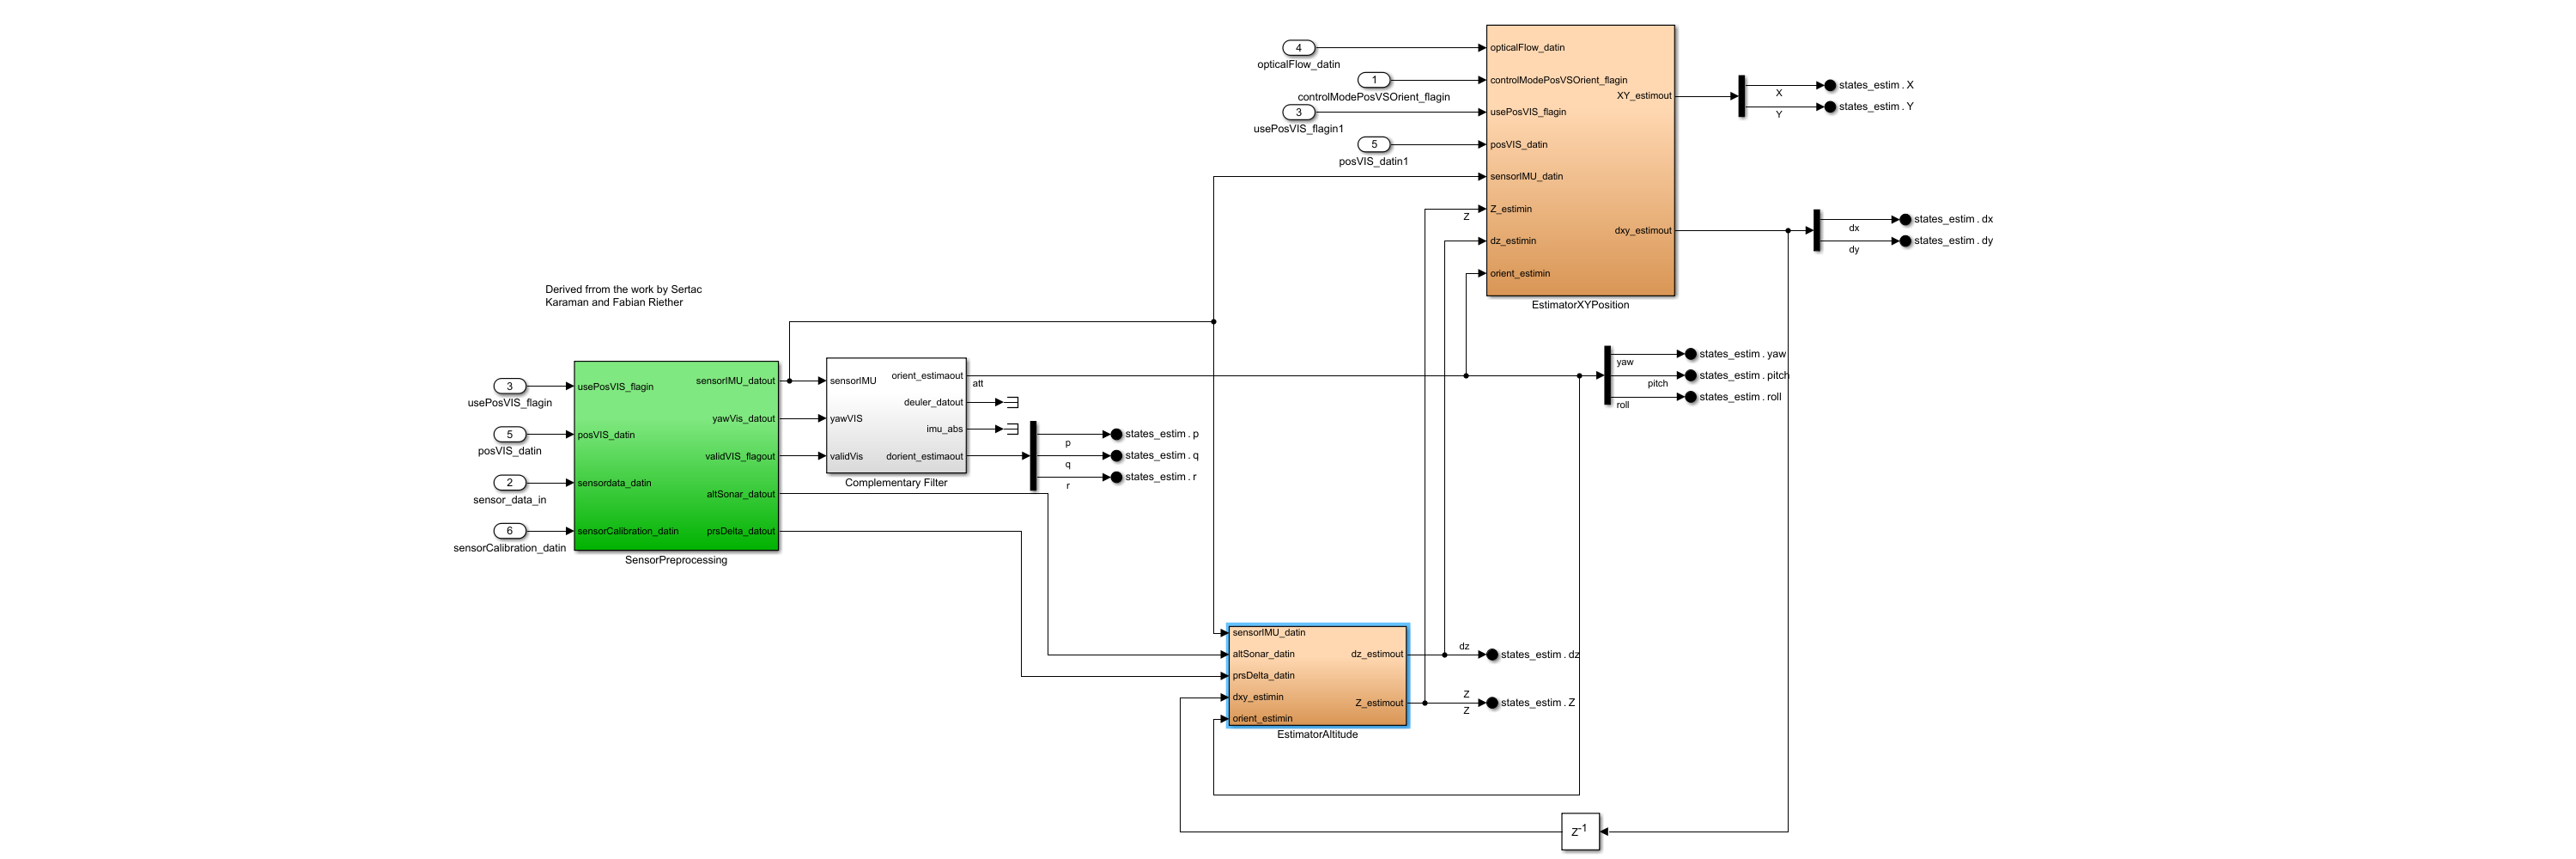
\includegraphics[width=1\textwidth]{flightControlSystem-estateestimator}
	\caption{Estimador de Estados}
	\centering
	\label{Estimador de Estados}
\end{figure}

A seguir ainda dentro do sistema de controle de voo, vamos entrar dentro do bloco do controlador, que é um dos blocos de interesse nesse trabalho.

\subsection{Controlador}

Olhando dentro do controlador, temos blocos importantes e que ainda serão explorados nesse trabalho afim de fazer melhorias no sistema de controle existente, por hora vamos apenas explica o que há em cada um dos blocos e como eles interagem entre si. 


\begin{figure}[H]
	\centering
	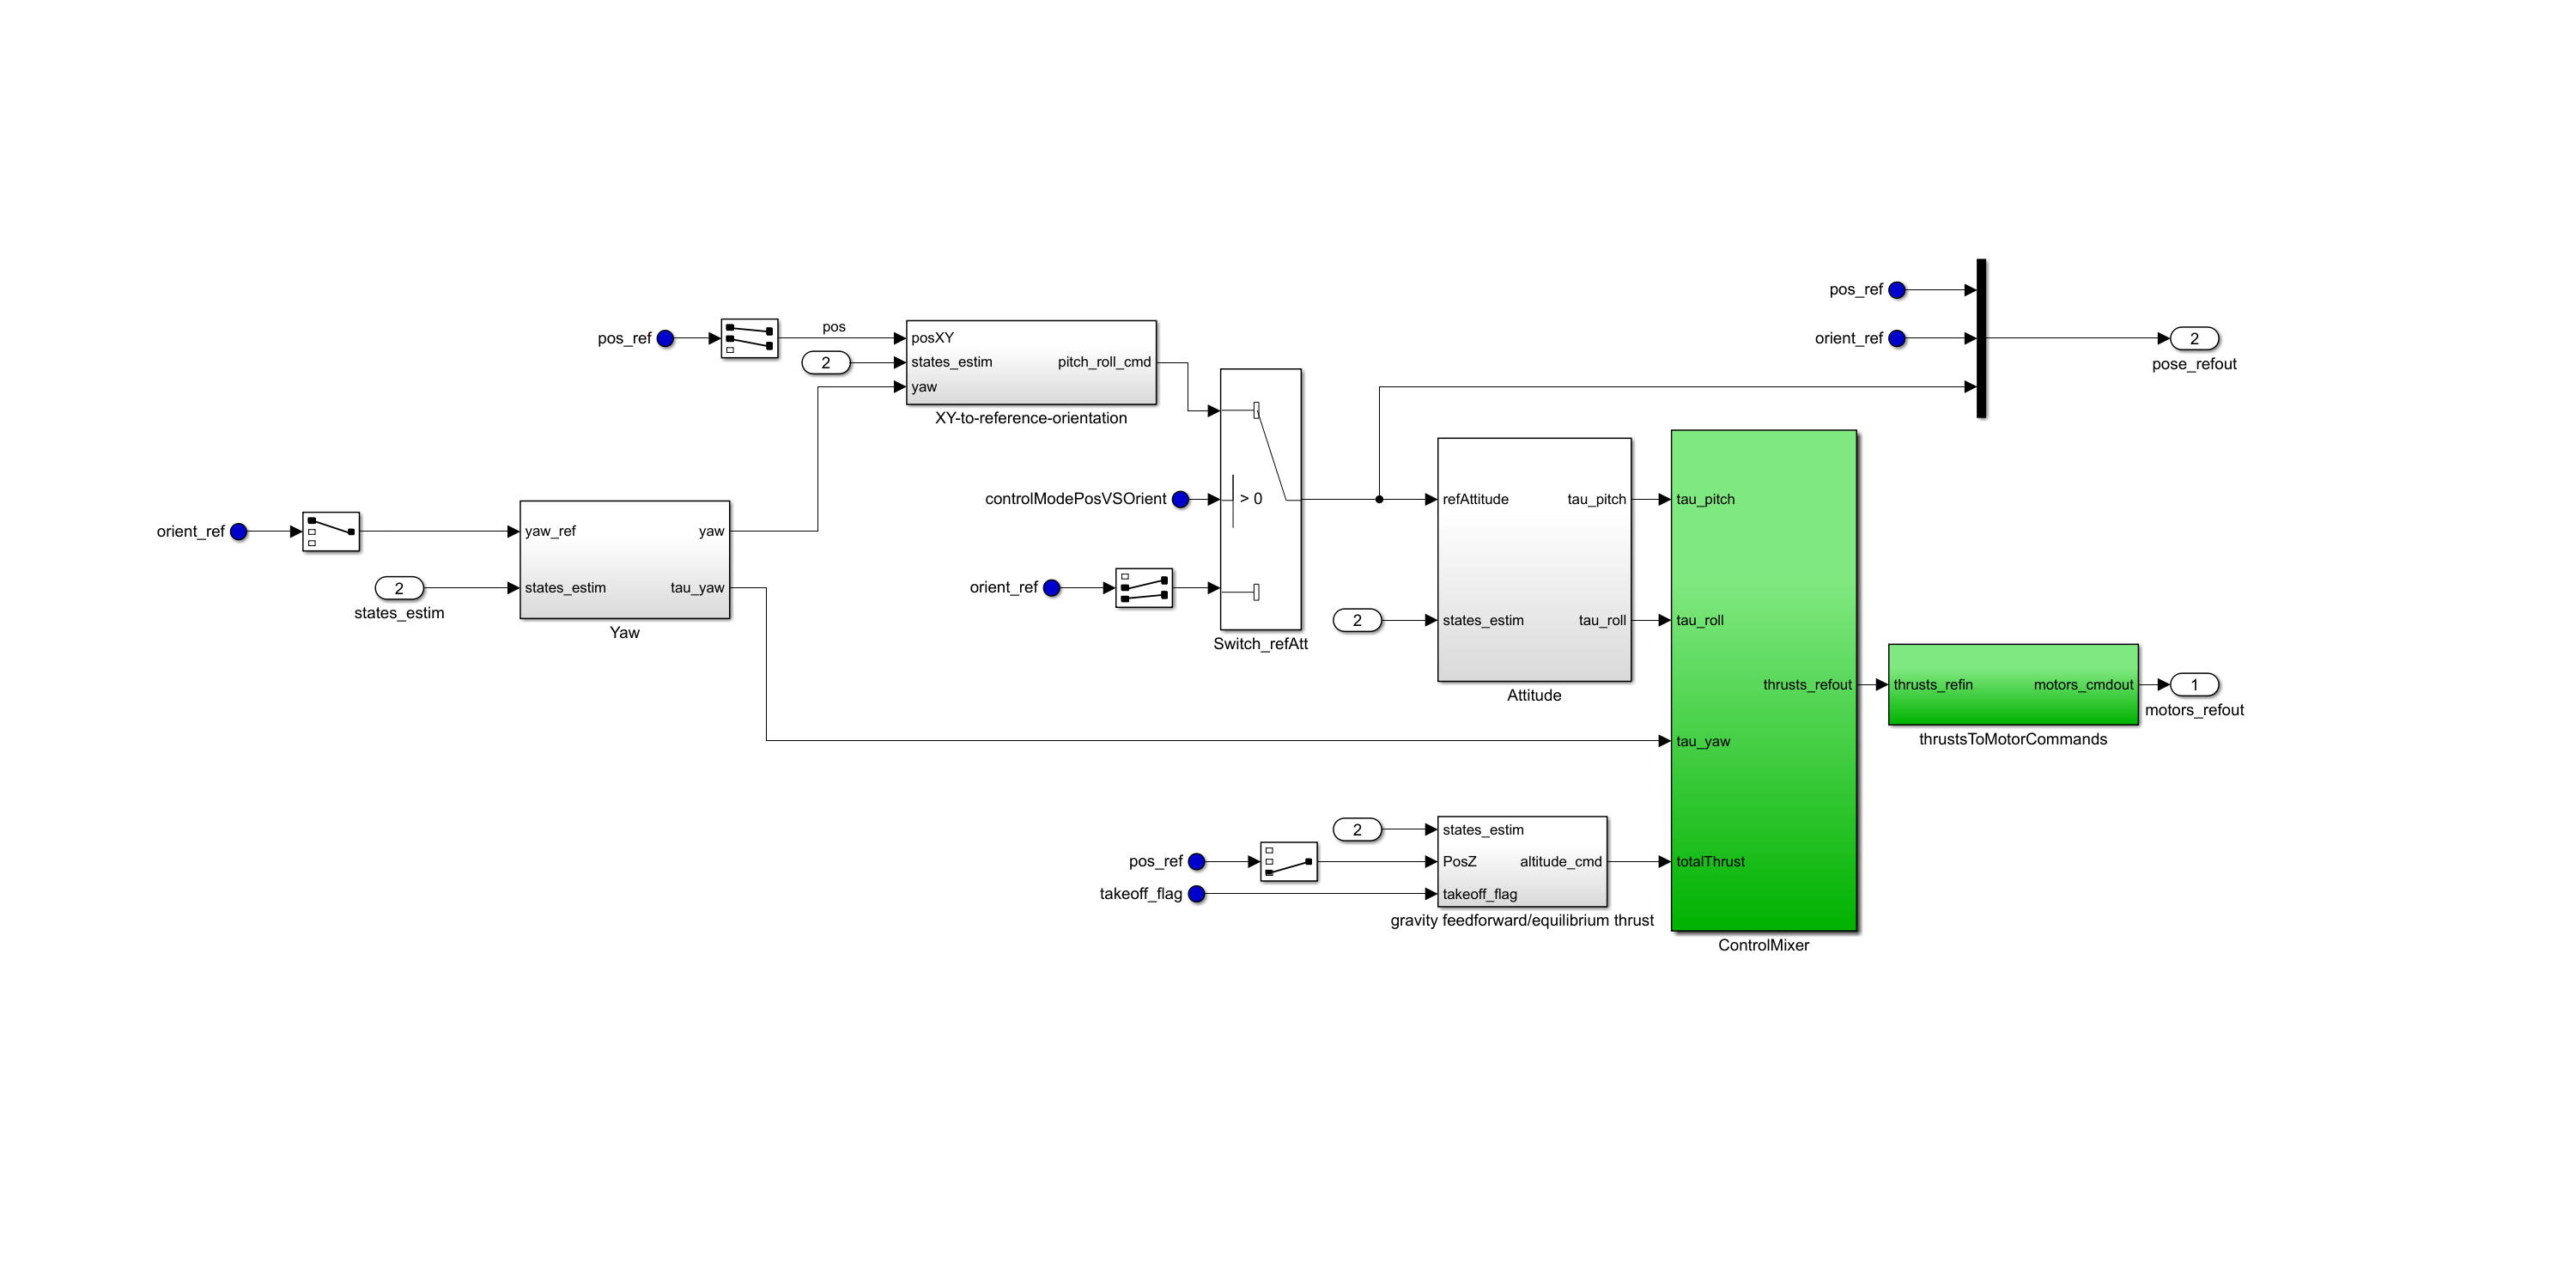
\includegraphics[width=0.8\textwidth]{flightControlSystem-controller}
	\caption{Controlador}
	\centering
	\label{Controlador}
\end{figure}

-Yaw - Controlador de guinada, tem o objetivo de calcular o torque necessário para que o quadricóptero atinja sua posição de guinada desejada. Faz isso através de um controlado PD, como podemos ver na imagem abaixo. Como o movimento de guinada não sofre influência ou sofre pouca influência dos movimentos de rolamento e arfagem, tem um controlador independente.

\begin{figure}[H]
	\centering
	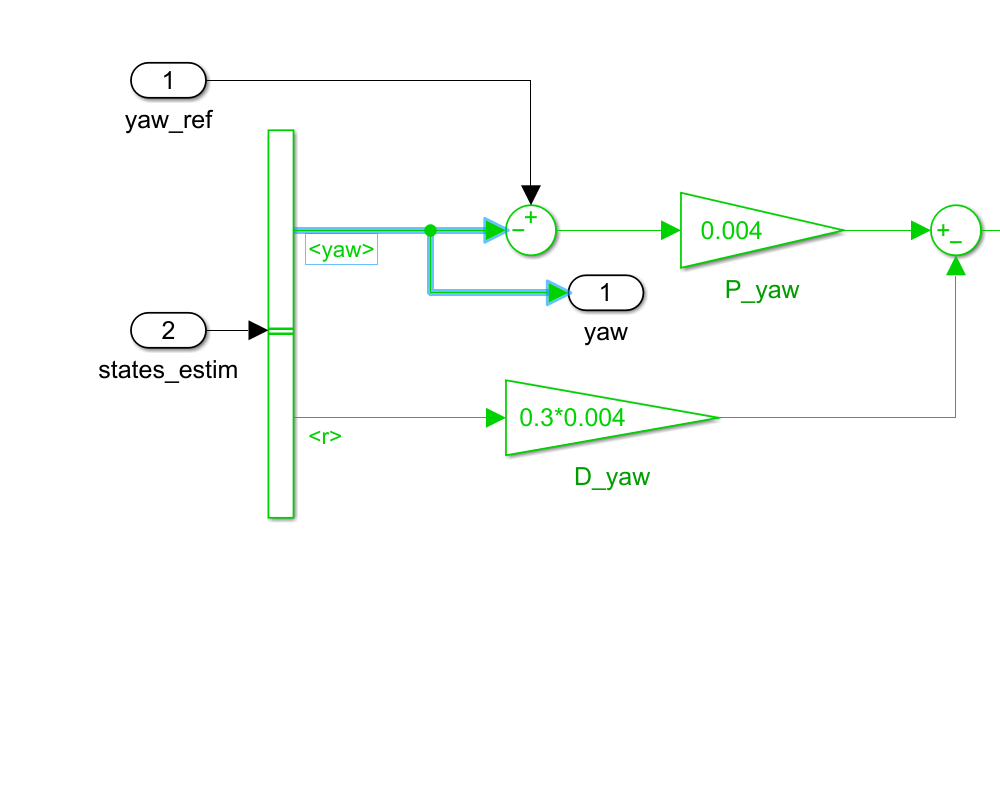
\includegraphics[width=0.8\textwidth]{flightControlSystem-controller-yaw}
	\caption{Controlador de Guinada}
	\centering
	\label{Controlador de Guinada}
\end{figure}

-XY to Reference Position - Tem o papel de calcular a atitude(angulo de rolamento e de arfagem) de referência do quadricóptero a partir da posição no plano XY e suas respectivas velocidades nessse plano, entretanto nem sempre esse calculo é usado, podemos ver que existe um bloco "switch", que valida se o valor é maior que zero, e caso não seja utiliza a orientação de referência calculada pelo estimador de estados que já foi falado anteriormente.

\begin{figure}[H]
	\centering
	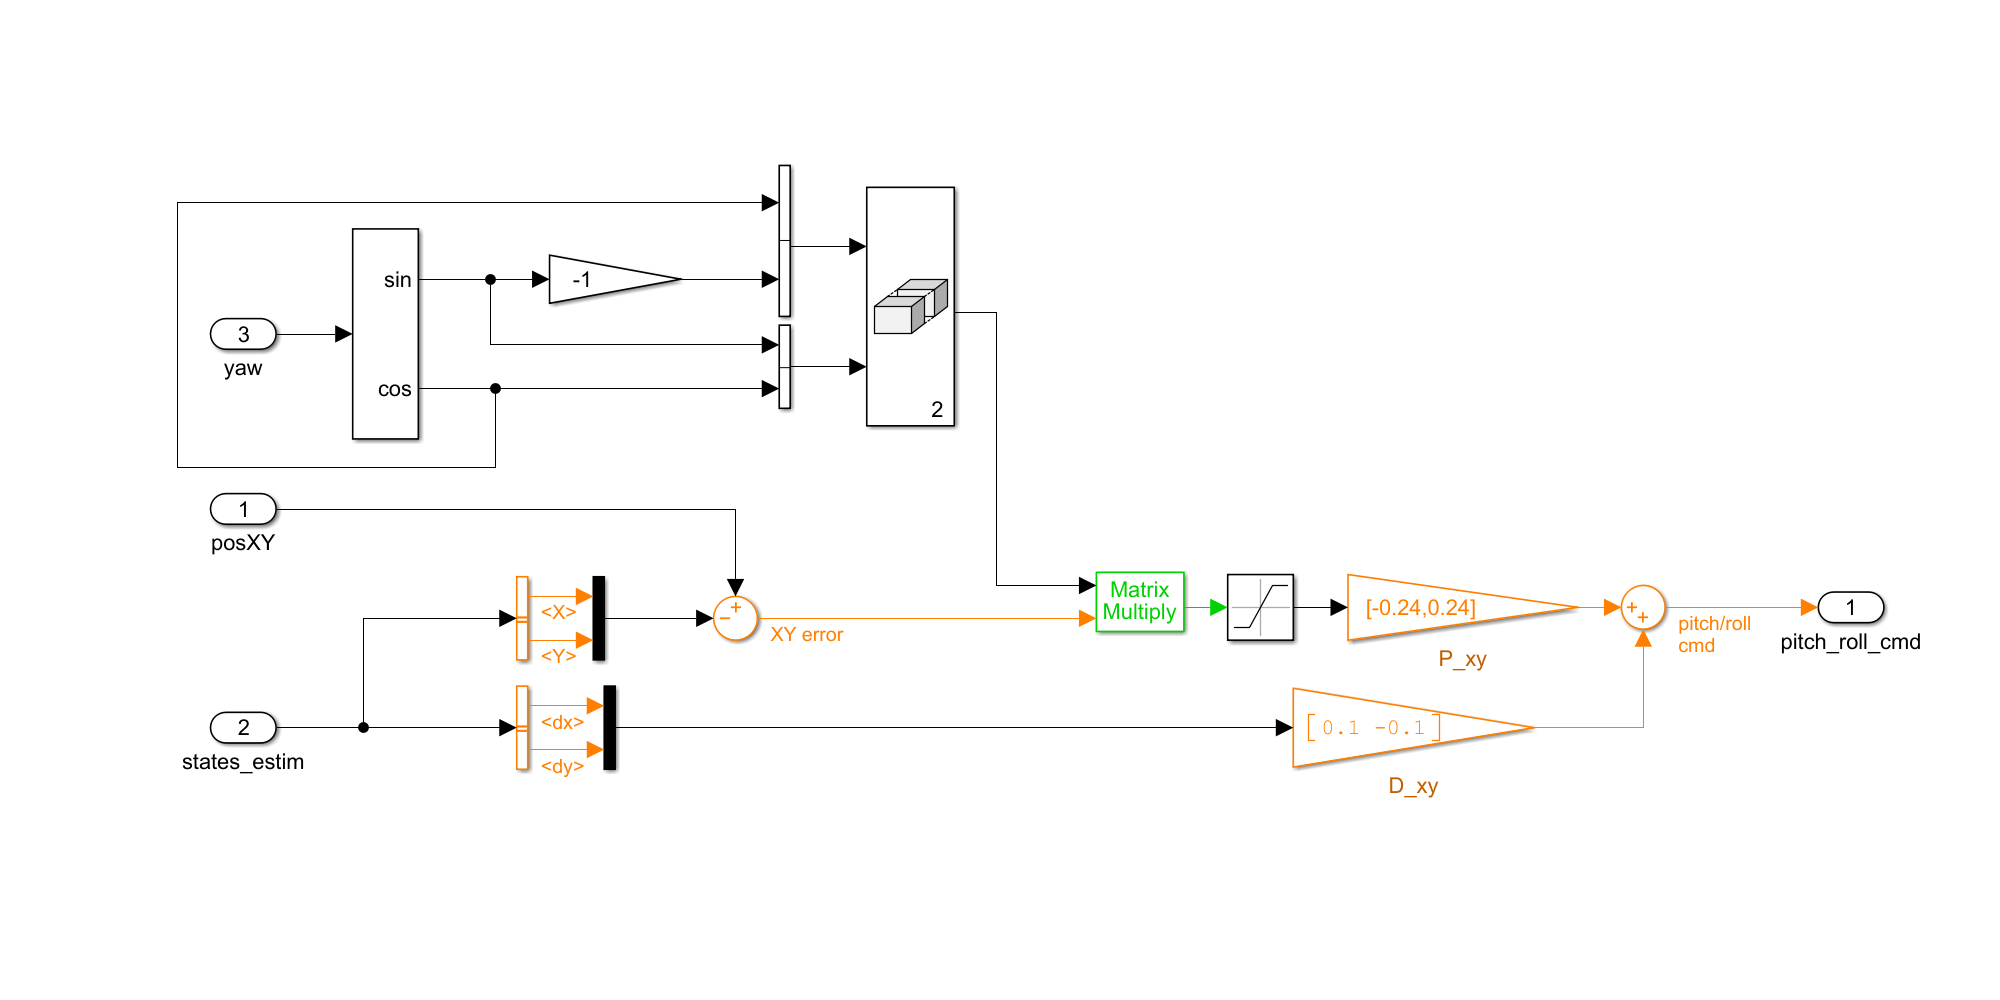
\includegraphics[width=0.8\textwidth]{flightControlSystem-controller-toReference}
	\caption{Estimador/Controlador de Atitude Primário}
	\centering
	\label{Estimador de Atitude}
\end{figure}

-Attitude - Controlador de atitude, tem como objetivo calcular os torques para controle de atitude do quadricóptero, e faz isso utilizando um controlador PID.

\begin{figure}[H]
	\centering
	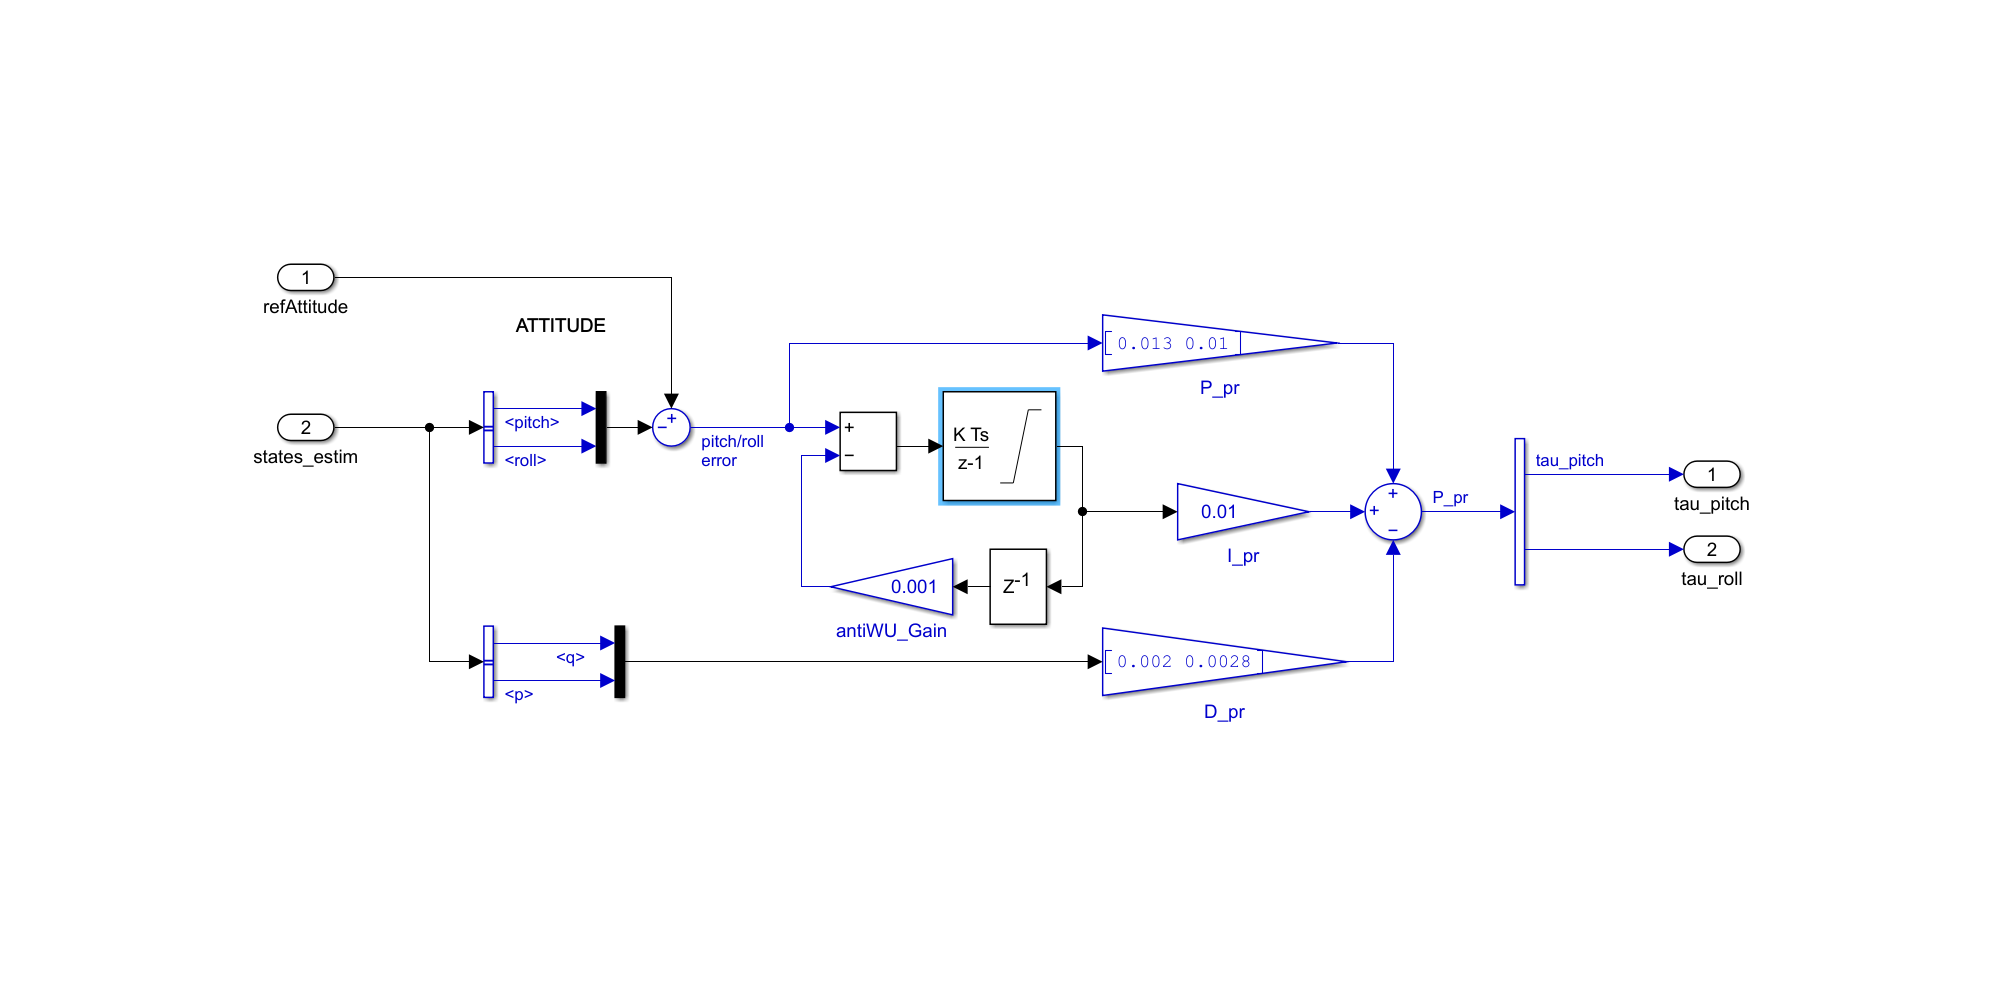
\includegraphics[width=1\textwidth]{flightControlSystem-controller-atitude}
	\caption{Controlador de Atitude}
	\centering
	\label{Controlador de Atitude}
\end{figure}


-Gravity feedforward/equilibrium thrust - Controlador de altitude,  tem como objetivo controlar a altitude do quadricóptero, e faz isso através de um controlador PD, calculando o empuxo necessário para atingir a altura desejada.

\begin{figure}[H]
	\centering
	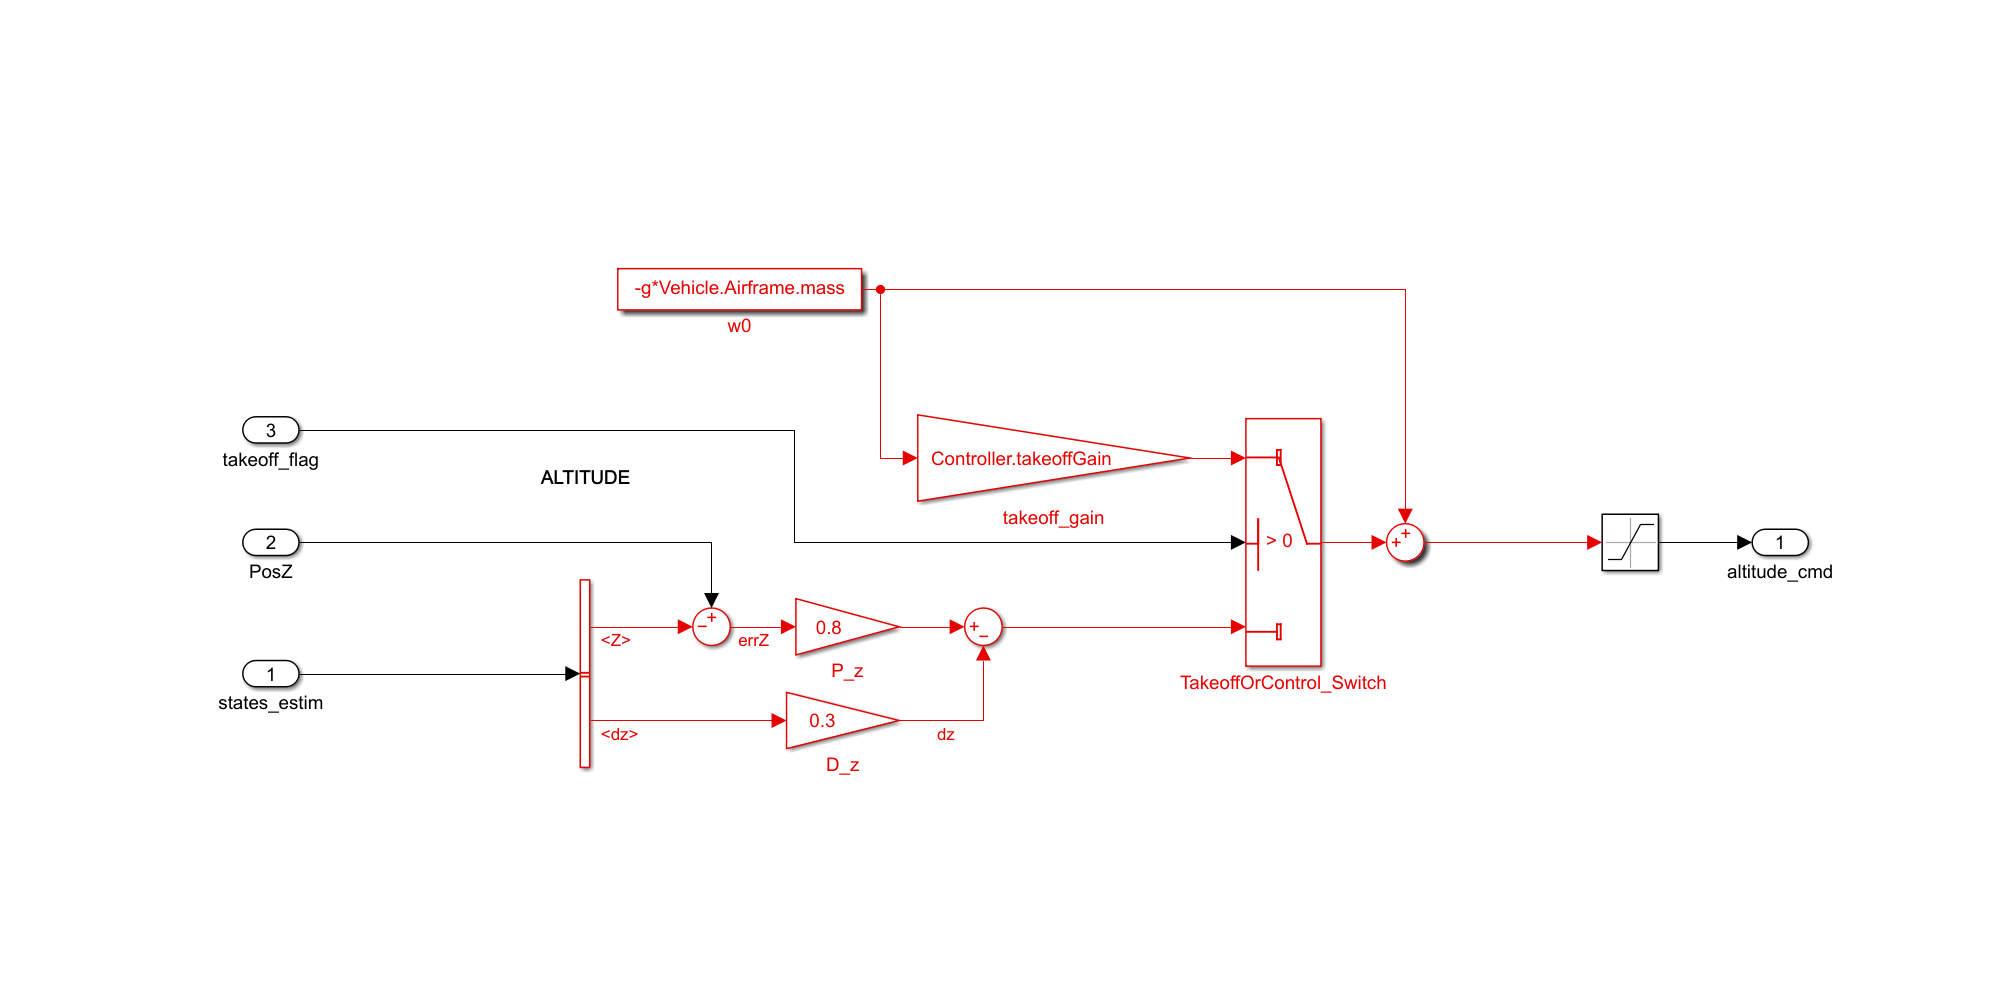
\includegraphics[width=0.8\textwidth]{flightControlSystem-controller-altitude}
	\caption{Controlador de Altitude}
	\centering
	\label{Controlador de Altitude}
\end{figure}

-Control Mixer - Junta as valores de torque necessário(torque de guinada, arfagem e rolamento) com o valor de empuxo para calcular o valor de empuxo necessário em cada motor. 

\begin{figure}[H]
	\centering
	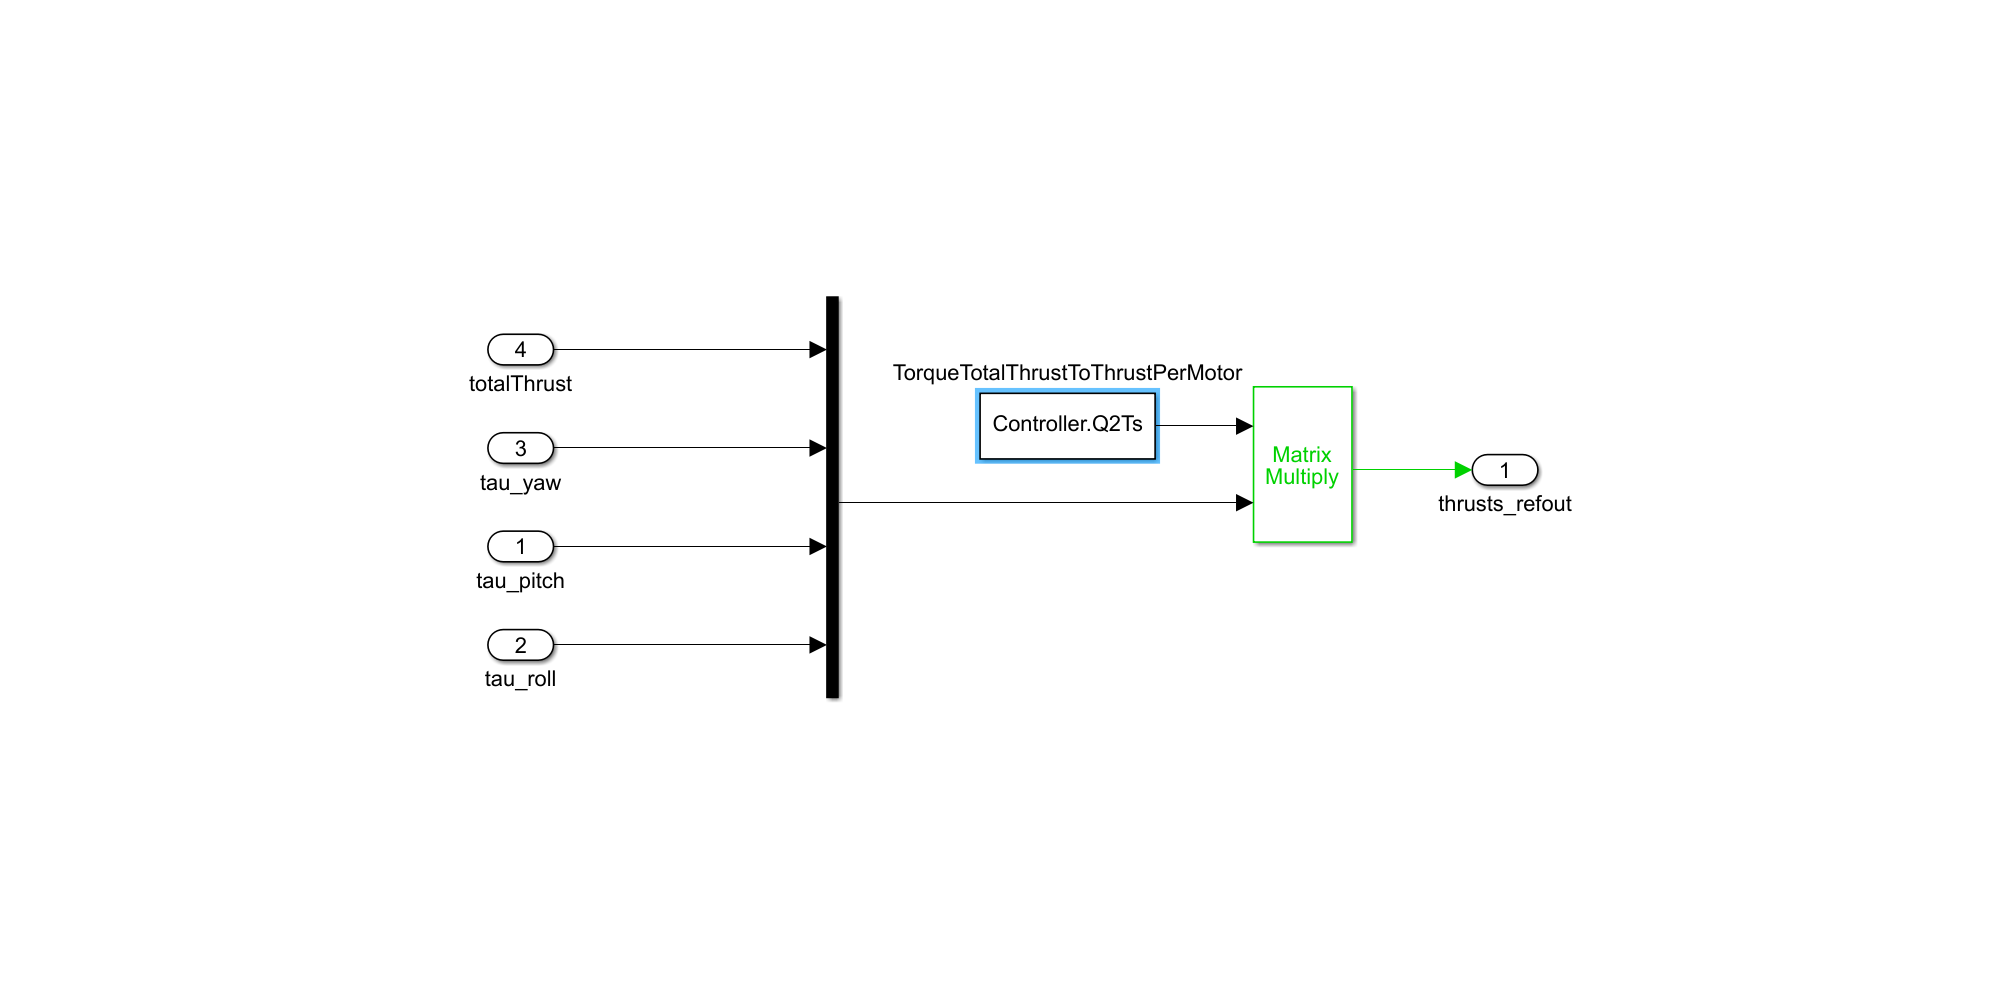
\includegraphics[width=1\textwidth]{flightControlSystem-controller-mixer}
	\caption{Agregador de Controle}
	\label{Agregador de Controle}
\end{figure}

-Thrusts To Motor Commands - Tem o objetivo de distribuir os empuxo necessário para os motores, transformando esses valores em comandos para os motores.

\begin{figure}[H]
	\centering
	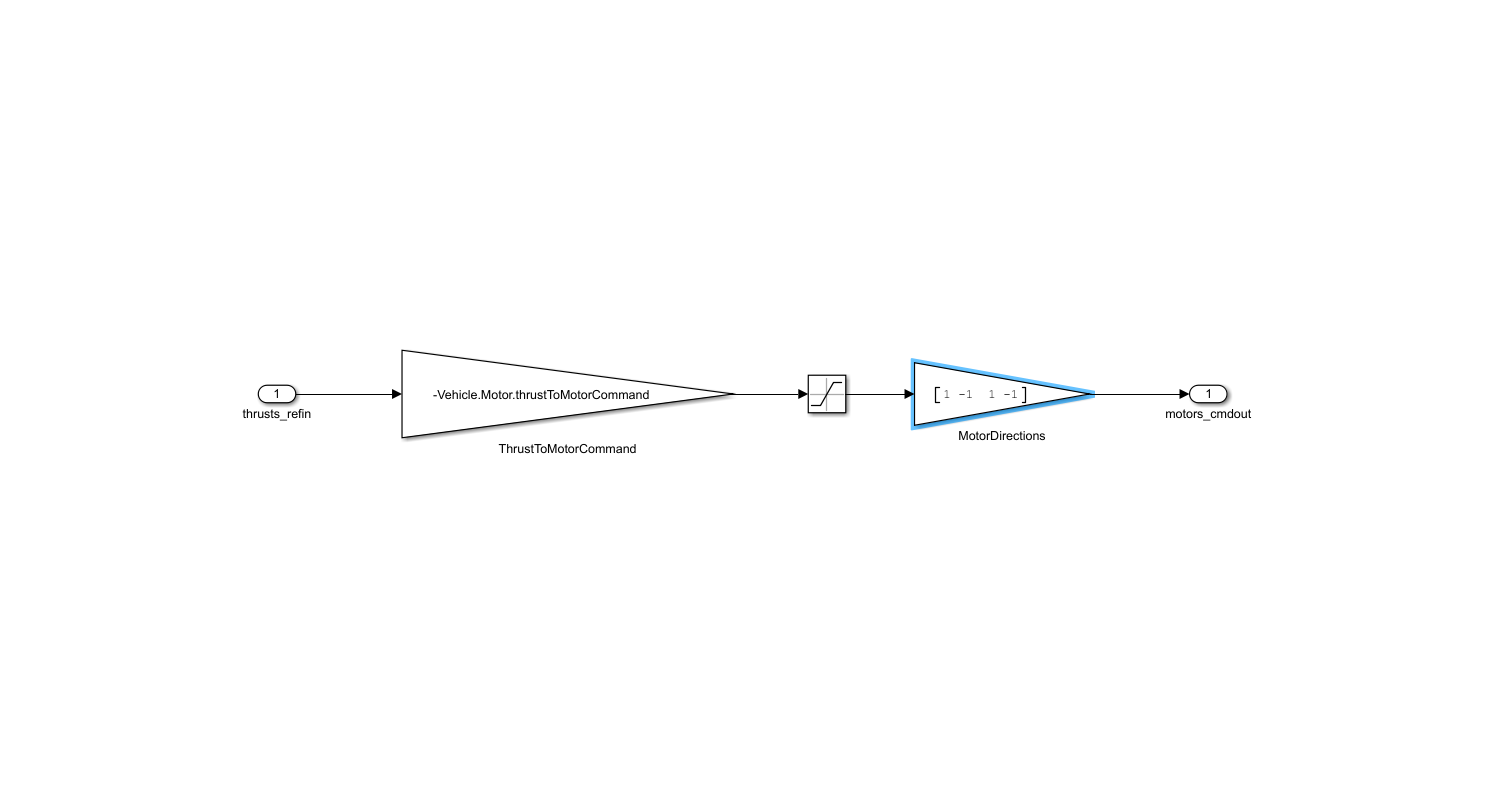
\includegraphics[width=0.8\textwidth]{flightControlSystem-controller-motorcmd}
	\caption{Transformador de Potência para Comandos de Motor}
	\centering
	\label{Transformador de Potência para Comandos de Motor}
\end{figure}


\section{Modelo do Quadricóptero no Matlab}

Nessa seção iremos analisar a planta do nosso sistema de controle, que no nosso caso, podemos nos referir como modelo dinâmico do quadricóptero. Na imagem abaixo podemos observar que temos duas opções de modelos para utilizar, um modelo linear e um modelo não linear, sendo que a alternancia entre modelos pode ser feita de forma simples alterando a variável \textit{VSSVEHICLE}.

Assim, iremos analisar a construção dos dois modelos e explicitar suas diferenças.

\begin{figure}[H]
	\centering
	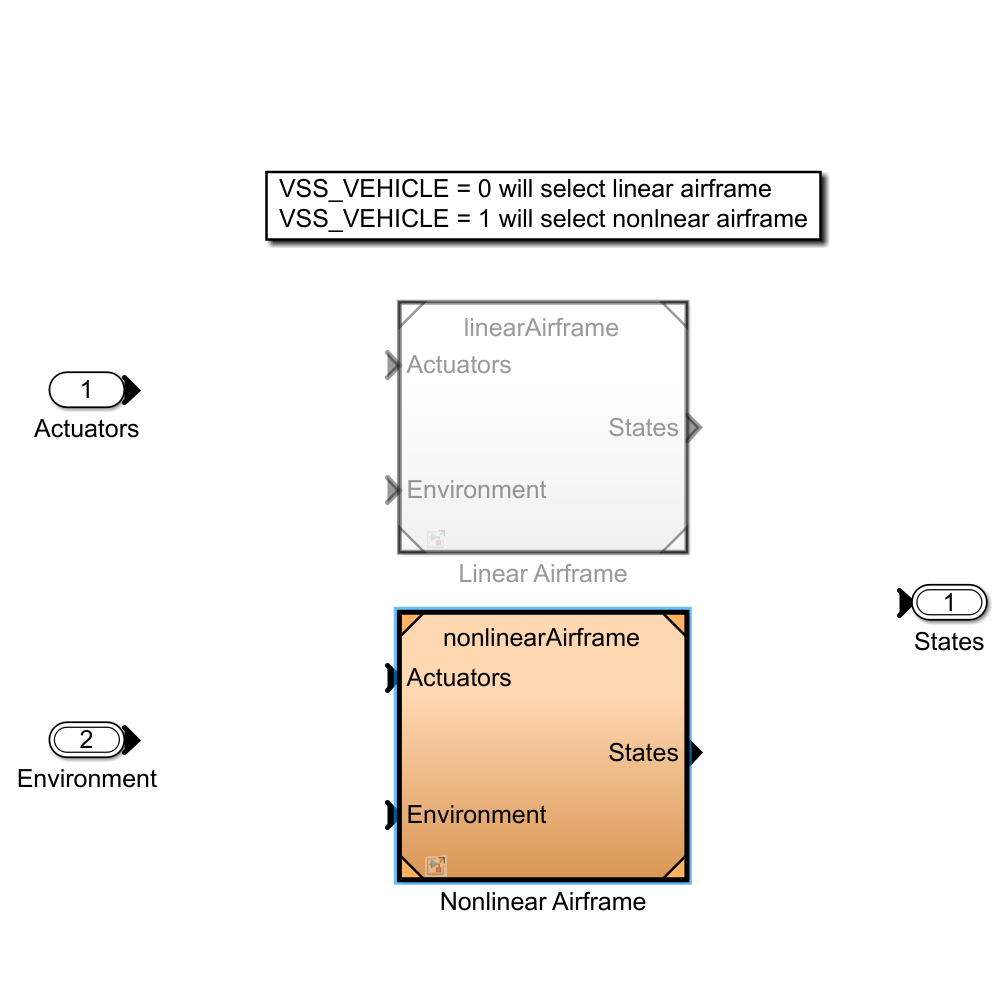
\includegraphics[width=1\textwidth]{asbQuadcopterProject - plant.png}
	\caption{Modelo dinâmico do quadricóptero}
	\centering
	\label{Modelo dinâmico do quadricóptero}
\end{figure}

-NonLinear Airframe - O modelo não linear do quadricóptero temos 2 subsistemas(blocos) importantes, o \textit{modelo AC}, que tem o papel de calcular as forças e momentos aerodiâmicos, sendo este o modelo dos atuadores e de como as perturbações do ambiente afetam o sistema e o \textit{6DOF(Ângulos de Euler)}, que recebe as forças e torques calculadas no \textit{modelo AC}, e integra as equações de movimento para obter os estados do quadricópteroa cada instante. O bloco 6DOF é uma representação de um corpo rígido que vêm do pacote  \textit{Aerospace blockset} do matlab e podemos selecionar o método de análise entre quaterinions e angulos de Euler.

\begin{figure}[H]
	\centering
	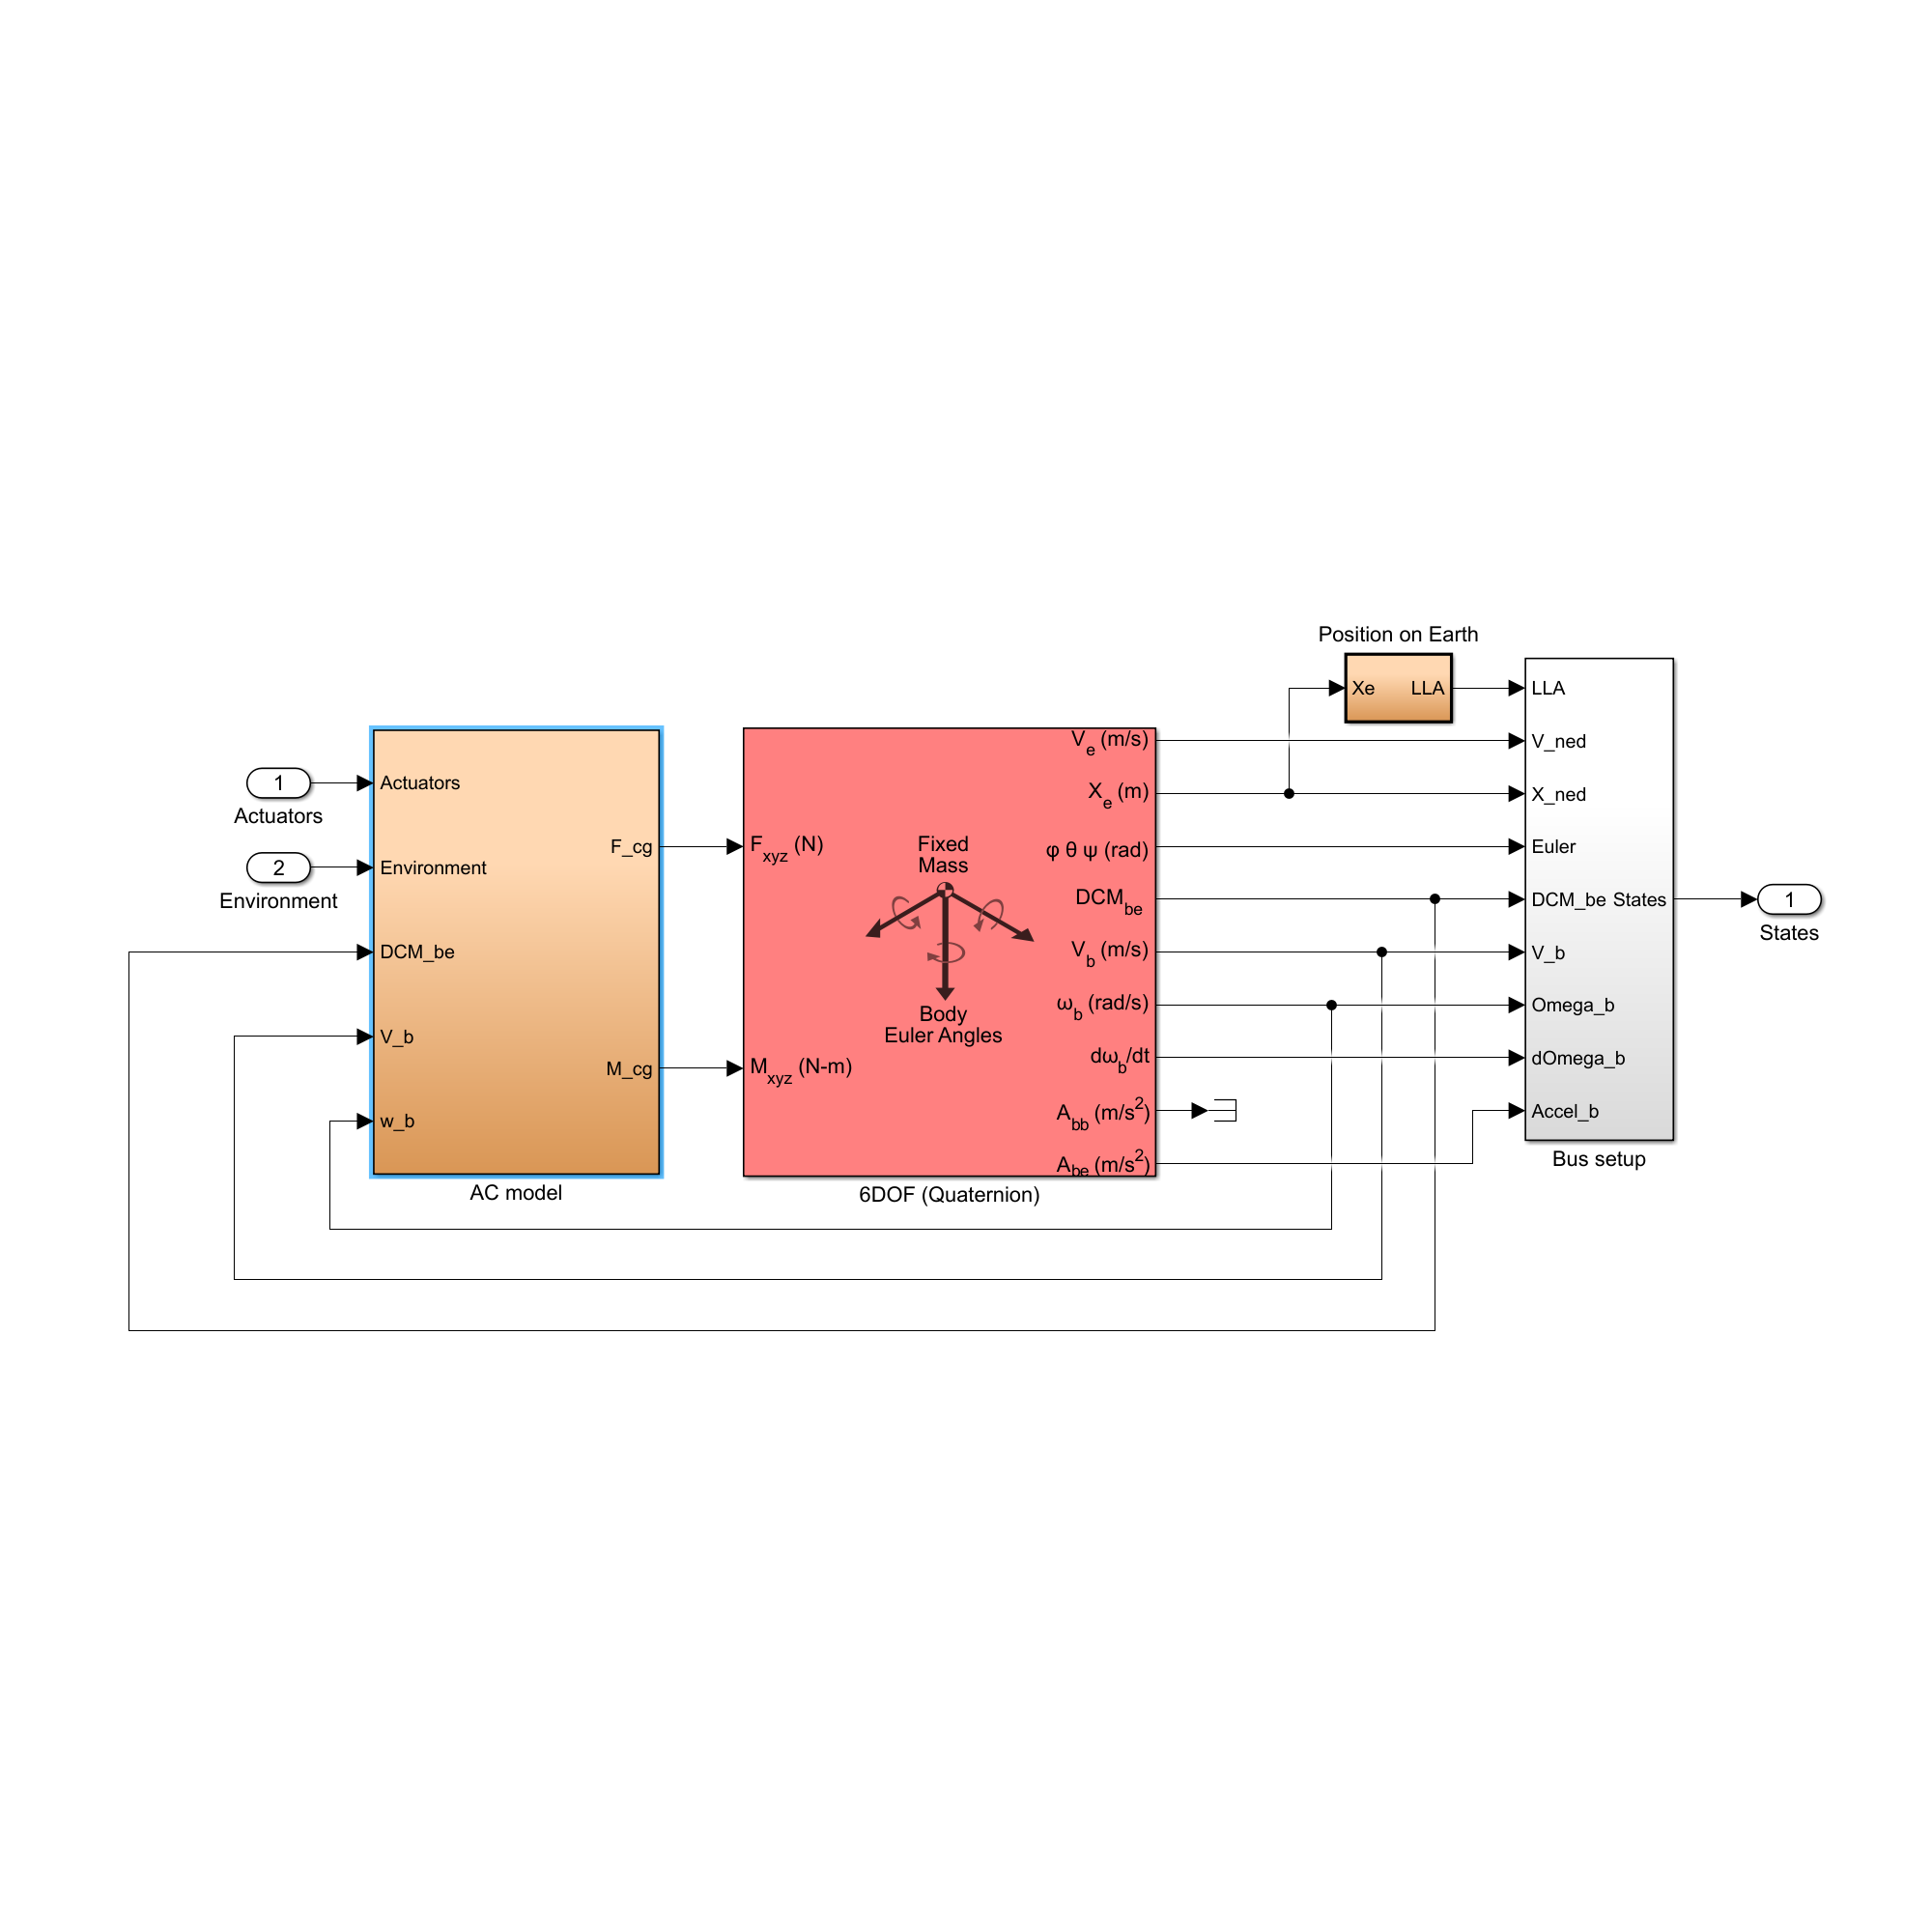
\includegraphics[width=1\textwidth]{asbQuadcopterProject - plant - nonLinear.png}
	\caption{Modelo não linear do Quadricóptero}
	\centering
	\label{Modelo não linear do Quadricóptero}
\end{figure}


\begin{figure}[H]
	\centering
	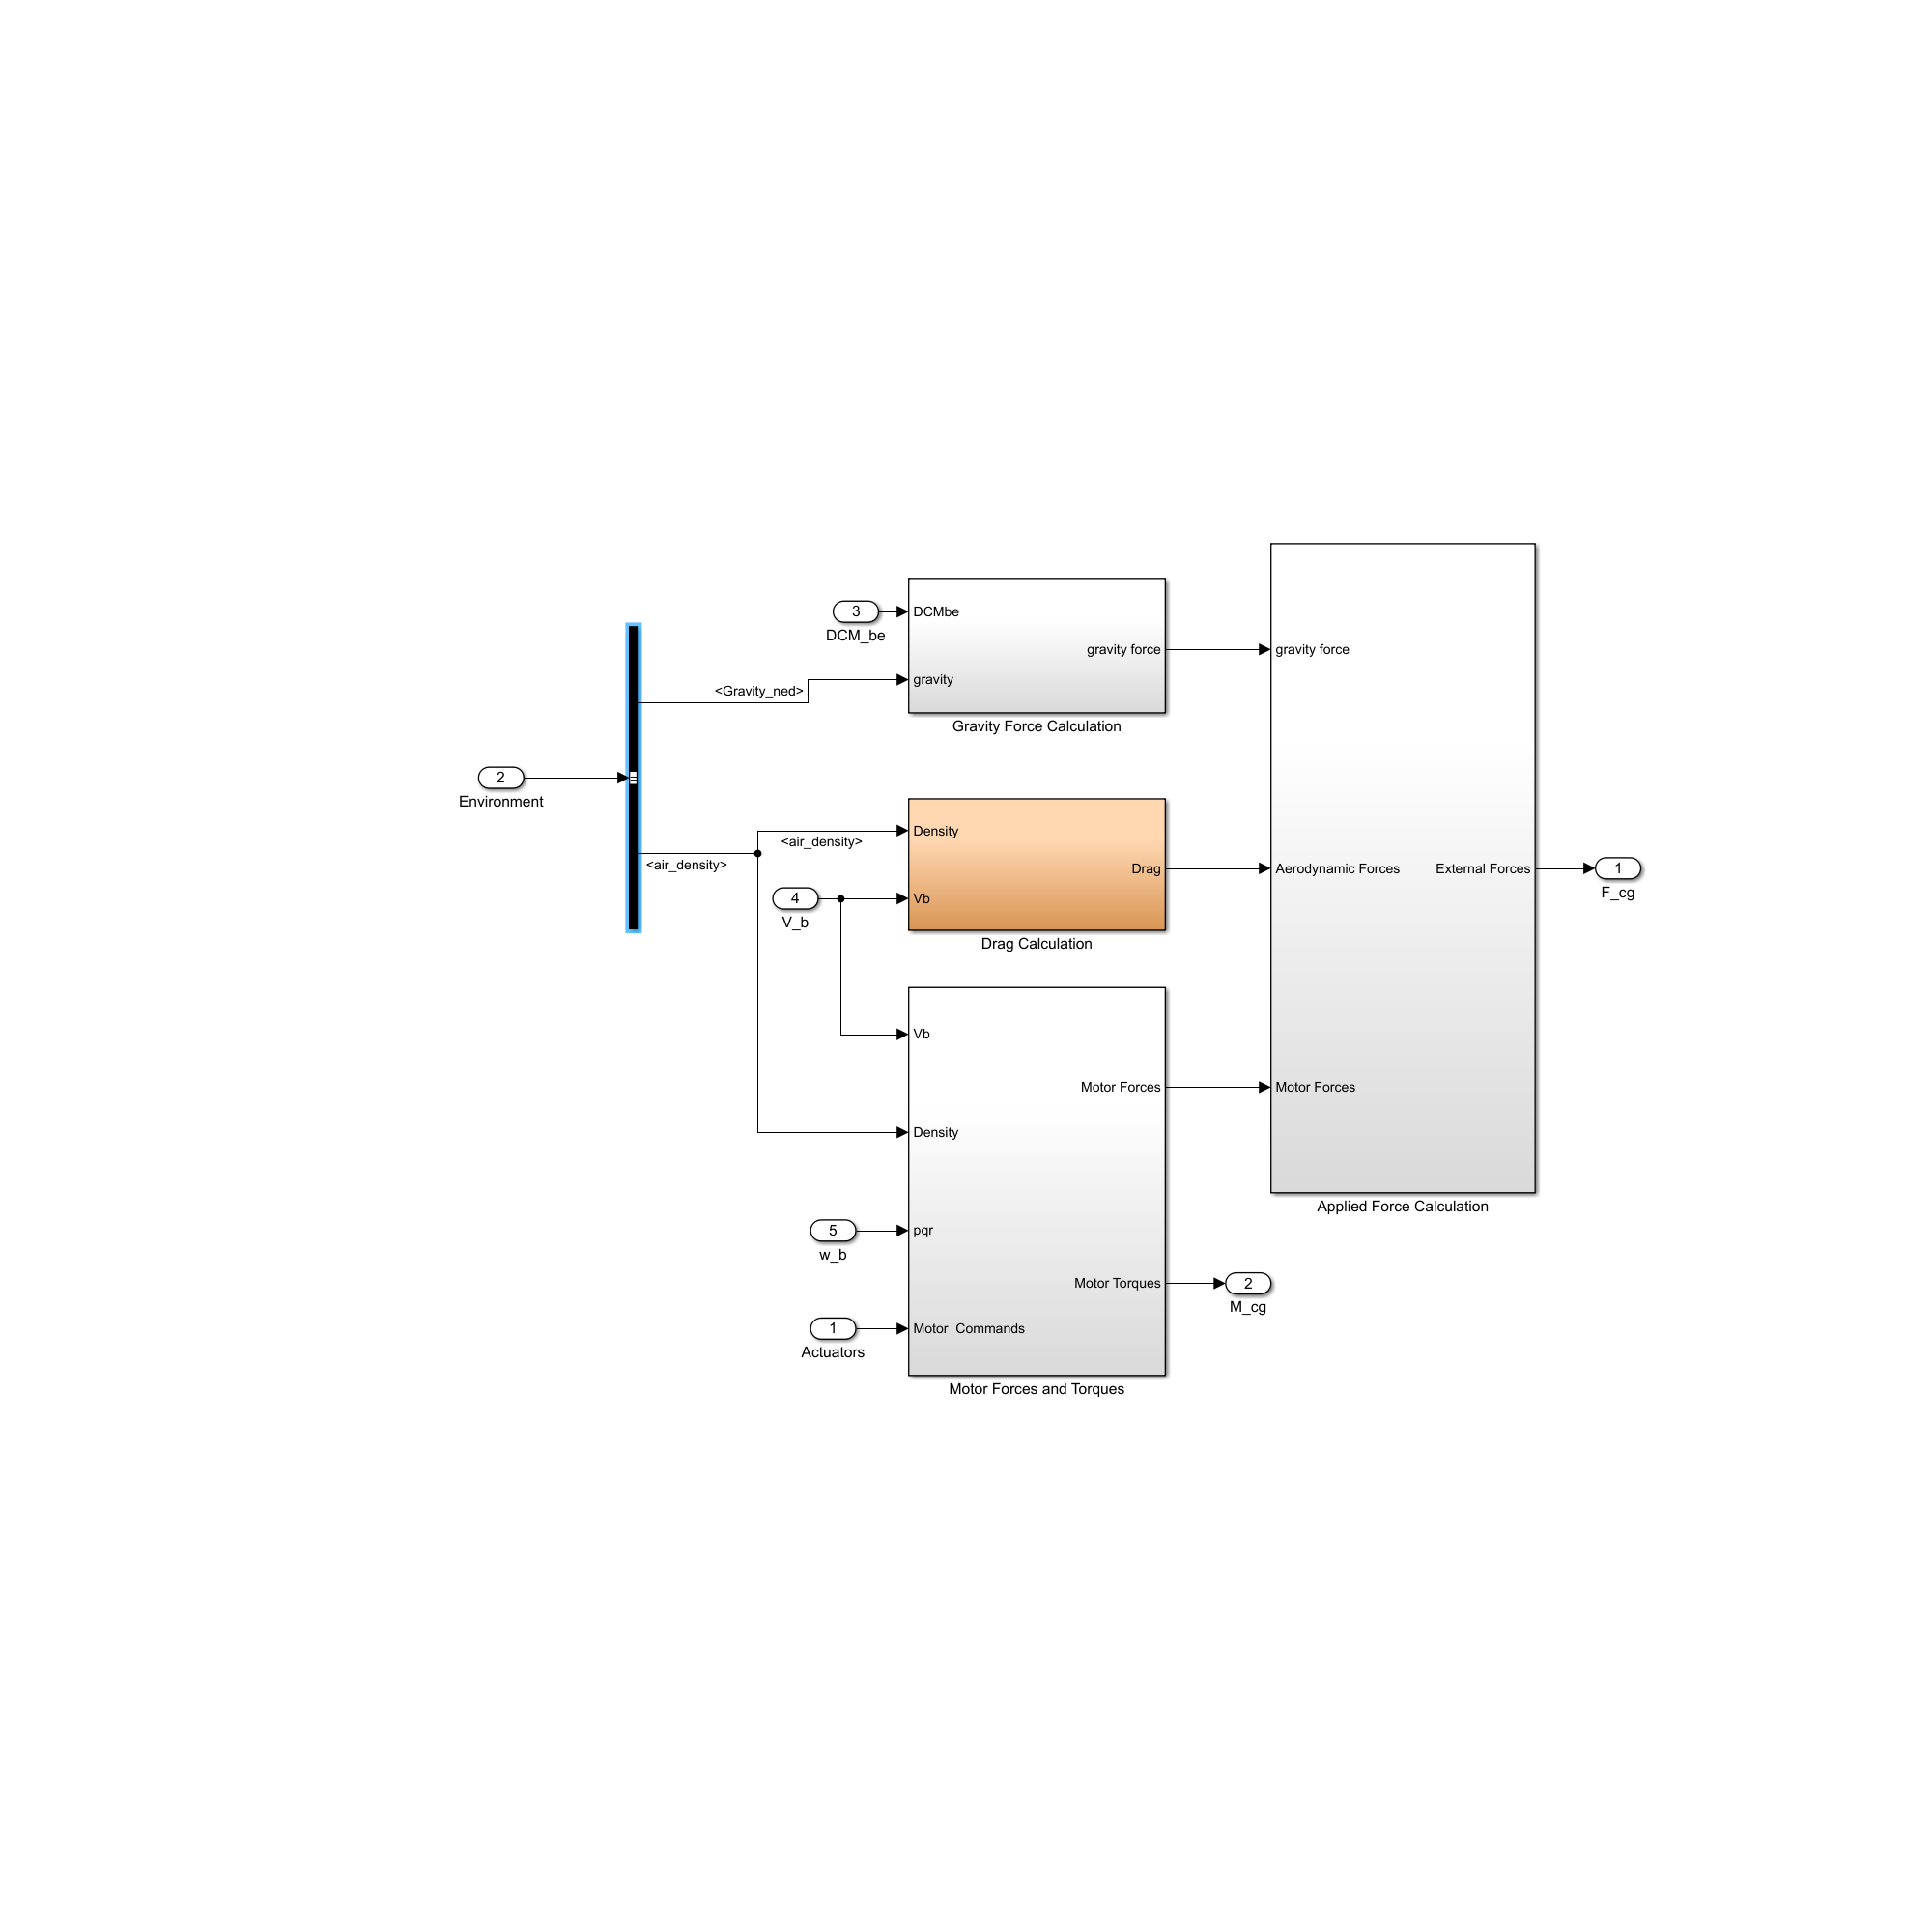
\includegraphics[width=1\textwidth]{asbQuadcopterProject - plant - nonLinear-ac-model.png}
	\caption{Modelo AC}
	\centering
	\label{Modelo AC}
\end{figure}



-Linear Airframe - O modelo linear nesse caso é o modelo não linear linearizado utilizando  Simulink® Control Design™, sendo que apesar do modelo linear ser menos preciso que o modelo não linear, ele é importante para podermos aplicar técnicas de otimização de controle linear.

\begin{figure}[H]
	\centering
	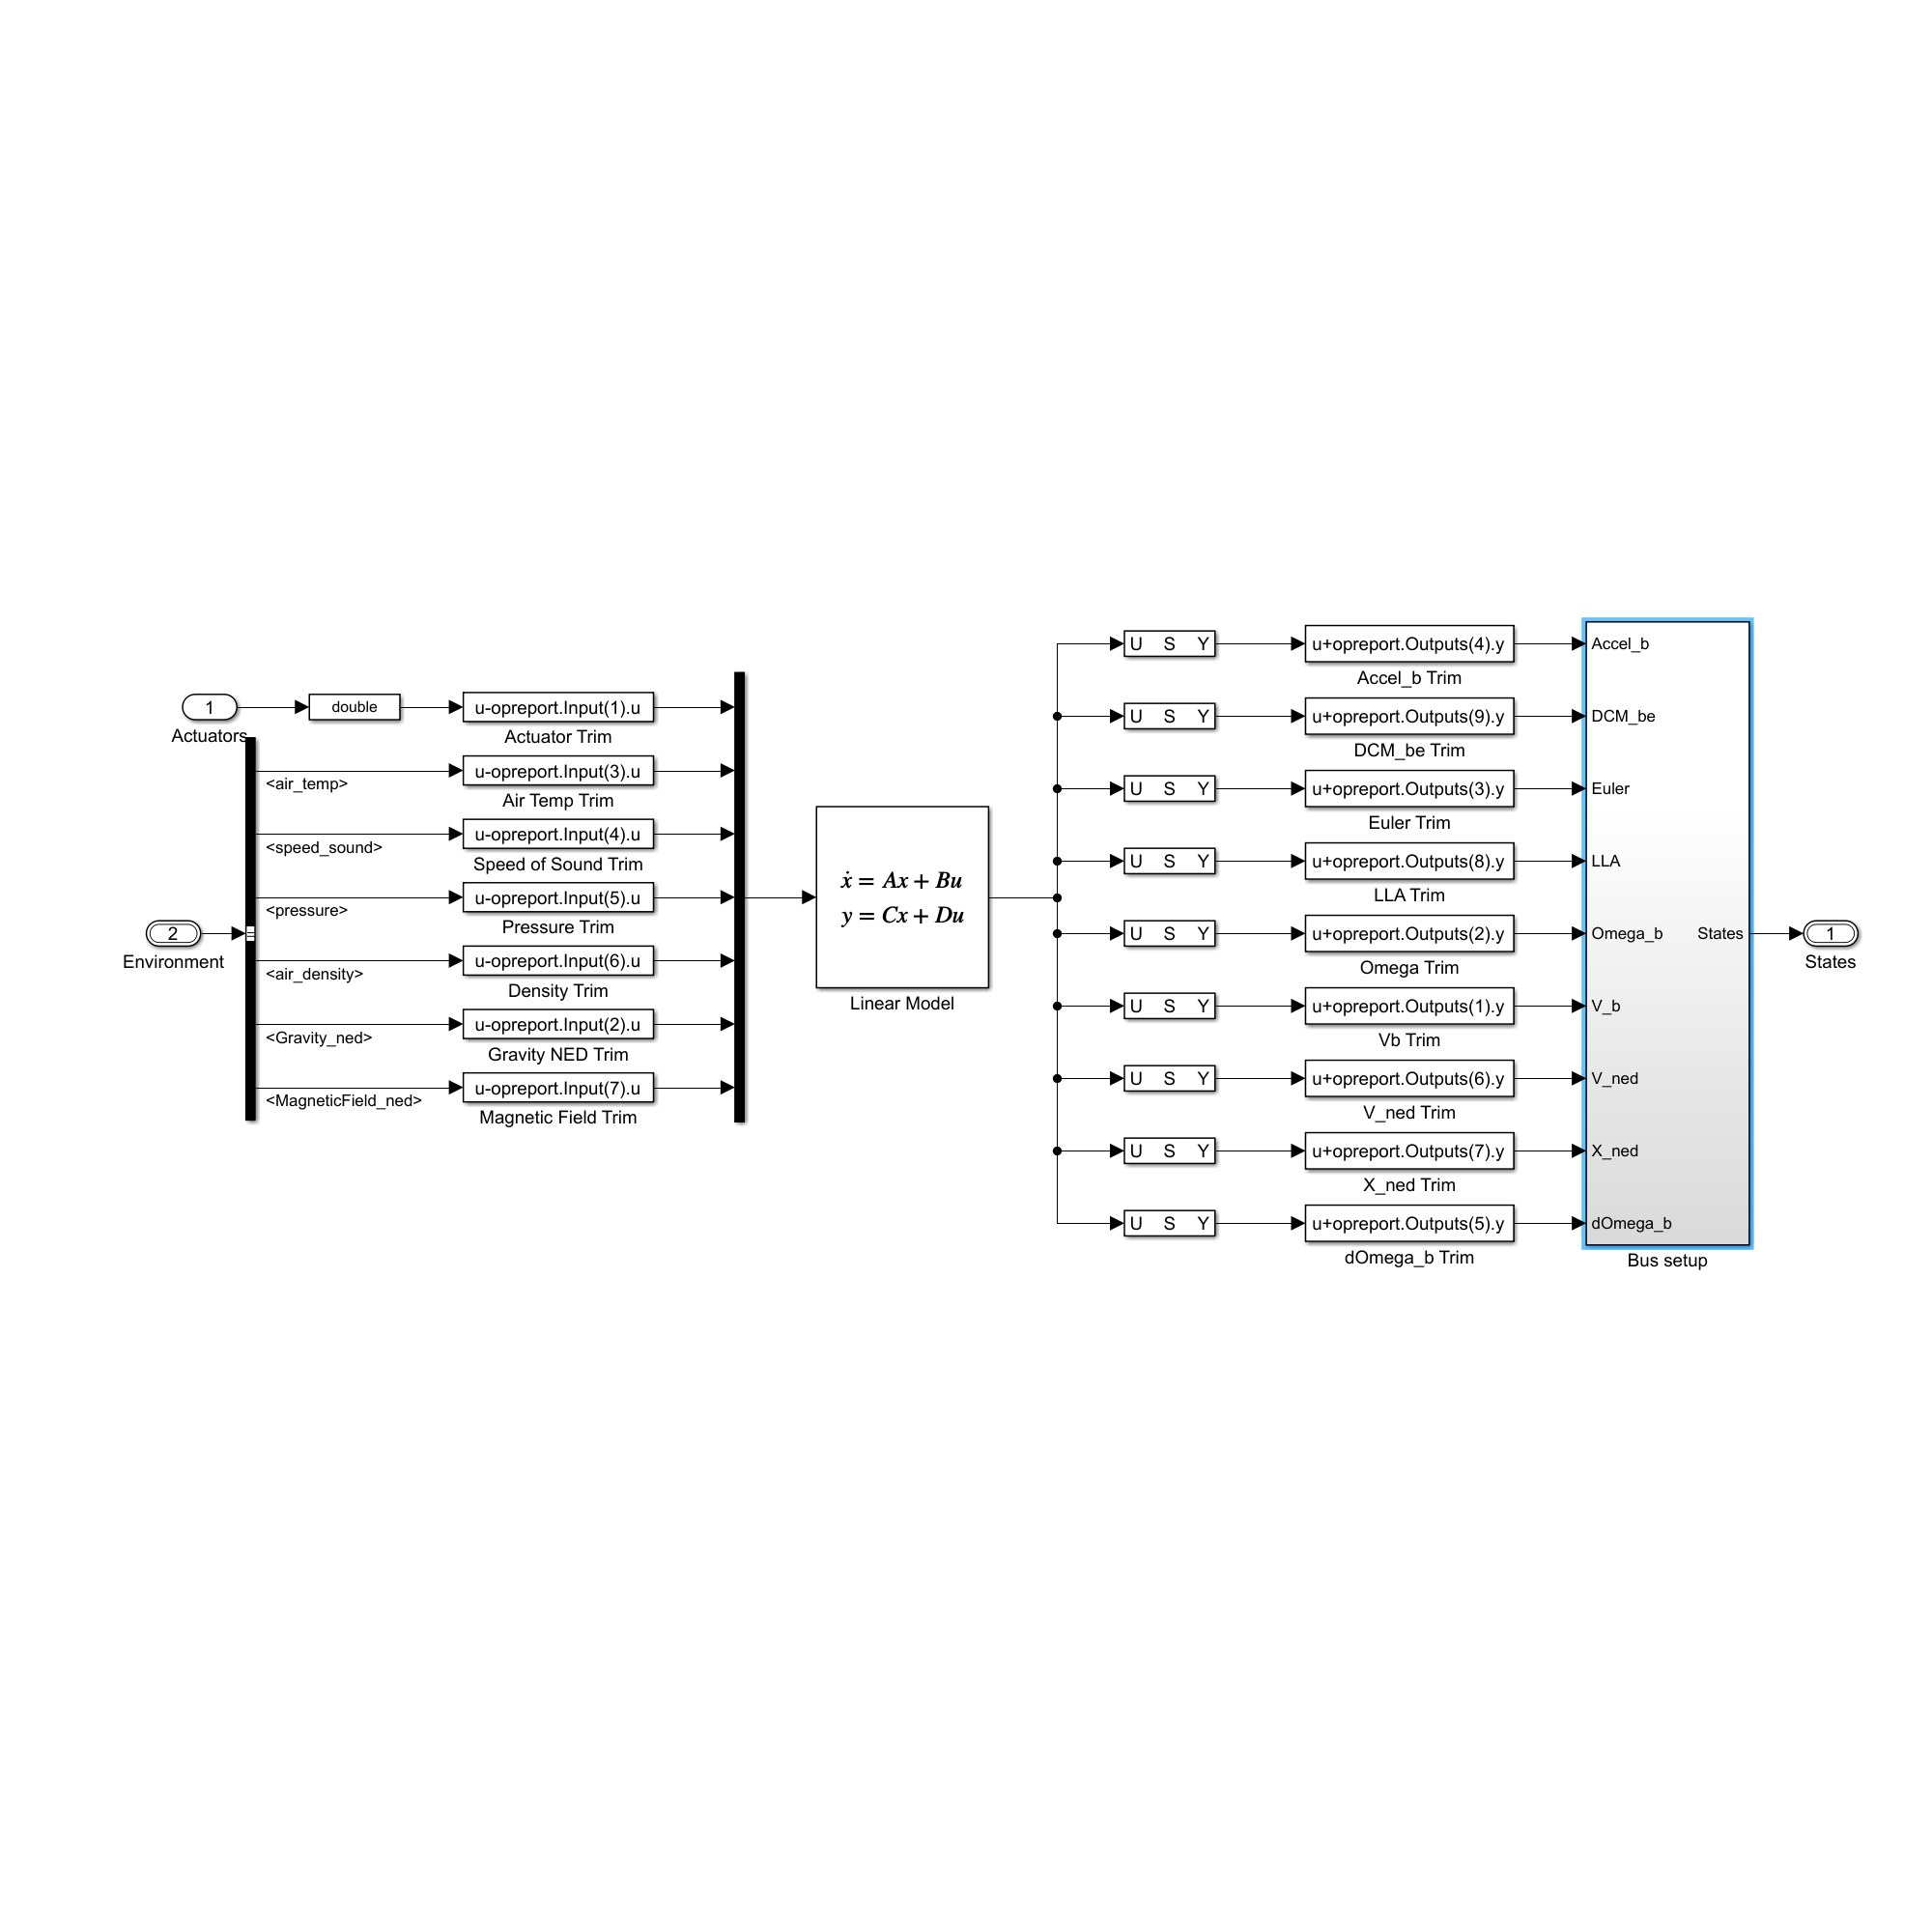
\includegraphics[width=1\textwidth]{asbQuadcopterProject - plant - linear.png}
	\caption{Modelo linear do Quadricóptero}
	\centering
	\label{Modelo linear do Quadricóptero}
\end{figure}
%---------------------------------------------------------------------
% INDICE REMISSIVO
%---------------------------------------------------------------------
\phantompart
\printindex
%---------------------------------------------------------------------


\chapter{\textit{Simulação e Controle}}

Este capítulo será dedicado a relacionar o que foi falado até o momento com o projeto disponibilizado pelo MATLAB e a Parrot. Dessa forma a simulação será executada para alguns cenários de interesse e serão gerados gráficos para análise de desempenho dos controladores atuais. Assim permitindo a proposta de melhorias onde for necessário.

\section{Configuração do Modelo no MATLAB Simulink}

Para configurar o modelo no MATLAB, existe uma documentação oficial no site da mathworks*adicionar citação*, que pode ser utilizada, mas além disso uma boa proposta é seguir o trabalho de LI, David, que apresenta um forma mais simples de configuração tanto para a simulação, quanto para testar o quadricóptero físico. Nesse trabalho o objetivo é trabalhar apenas com a simulação, então para iniciar a simulação deve-se rodar o comando \textit{asbQuadcopterStart} no MATLAB, após instalar as dependências necessárias. É importante notar que a princípio as modificações que são feitas no projeto não têm nenhum intuito de melhorar a performance dos controladores ou o desempenho do modelo as configuraçôes que serão citadas a seguir só tem o papel de deixar o modelo pronto para executar as simulações com as entradas que vamos inserir e facilitar a obtenção das saídas de forma que possamos coloca-las em gráficos e realizar a análise.

\subsection{Configurando Entradas e Saídas}

Uma trajetória de voo, pode ser completamente descrita, sabendo como as coordenadas em x, y e z e a guinada do quadricóptero se comportam durante o tempo de simulação, mas como já falado na seção de controle os ângulos de rolagem e arfagem são mais importantes do que as coordenadas em x e y, quando queremos controlar o quadricóptero. Assim, é interesse desse trabalho observar o comportamento dos seis graus de liberdade que existem na simulação, as coordenadas em x, y e z, bem como rolagem, arfagem e guinada. 

\subsubsection{Configuração das entradas}

Esse modelo oferece quatro possíveis forma de entrada, Editor de Sinal, Joystick, Dados(em arquivo no formato .mat), planilha de dados(dados no formato .xlsx). Aqui como sugerido por David Li, vamos utilizar apenas editor de sinais para criar os cenários de simulação, após fazer algumas modificações necessárias para permitir a implementação correta no Simulink.

\subsubsection{Configuração de Saída}

Para as saídas, o modelo inclui estados estimados e valores de referência. No entanto, foram adicionados blocos extras, conforme descrito por Li \cite{li2022}, para incluir os valores de estado "verdadeiros" na simulação, permitindo uma comparação mais completa entre os valores estimados e simulados.

 
\section{Simulação e Resultados}

Nessa seção será apresentada a técnica utilizada para realizar as simulações, bem como os resultados obtidos na simulação.

\subsection{Simulação}

O projeto já têm dois cenários para simulação prontos dentro do bloco de edição de sinais, \textit{Hover}(Voo pairado) e \textit{Landing Search}(Voo buscando um local pré determinado para pouso). O cenário \textit{Landing Search}, não é do nosso interesse no momento pois é um cenário mais complexo, onde o drone utiliza a câmera para procurar um ponto vermelho onde deveria pousar. Como nosso interesse é estudar e entender o desempenho dos contralores, a melhor forma de obter esses resultados é com cenários mais simples como \textit{Hover}, *adicionar cenários que vão ter simulados*.

\subsubsection{Criando cenários}

Para criação ou edição de algum cenário existente, precisamos acessar o \textit{Signal Editor}, abrir o bloco \textit{Position/Attitude Reference}, e clicar no botão circulado em vermelho que abrirá o editor de sinais.


\begin{figure}[H]
	\centering
	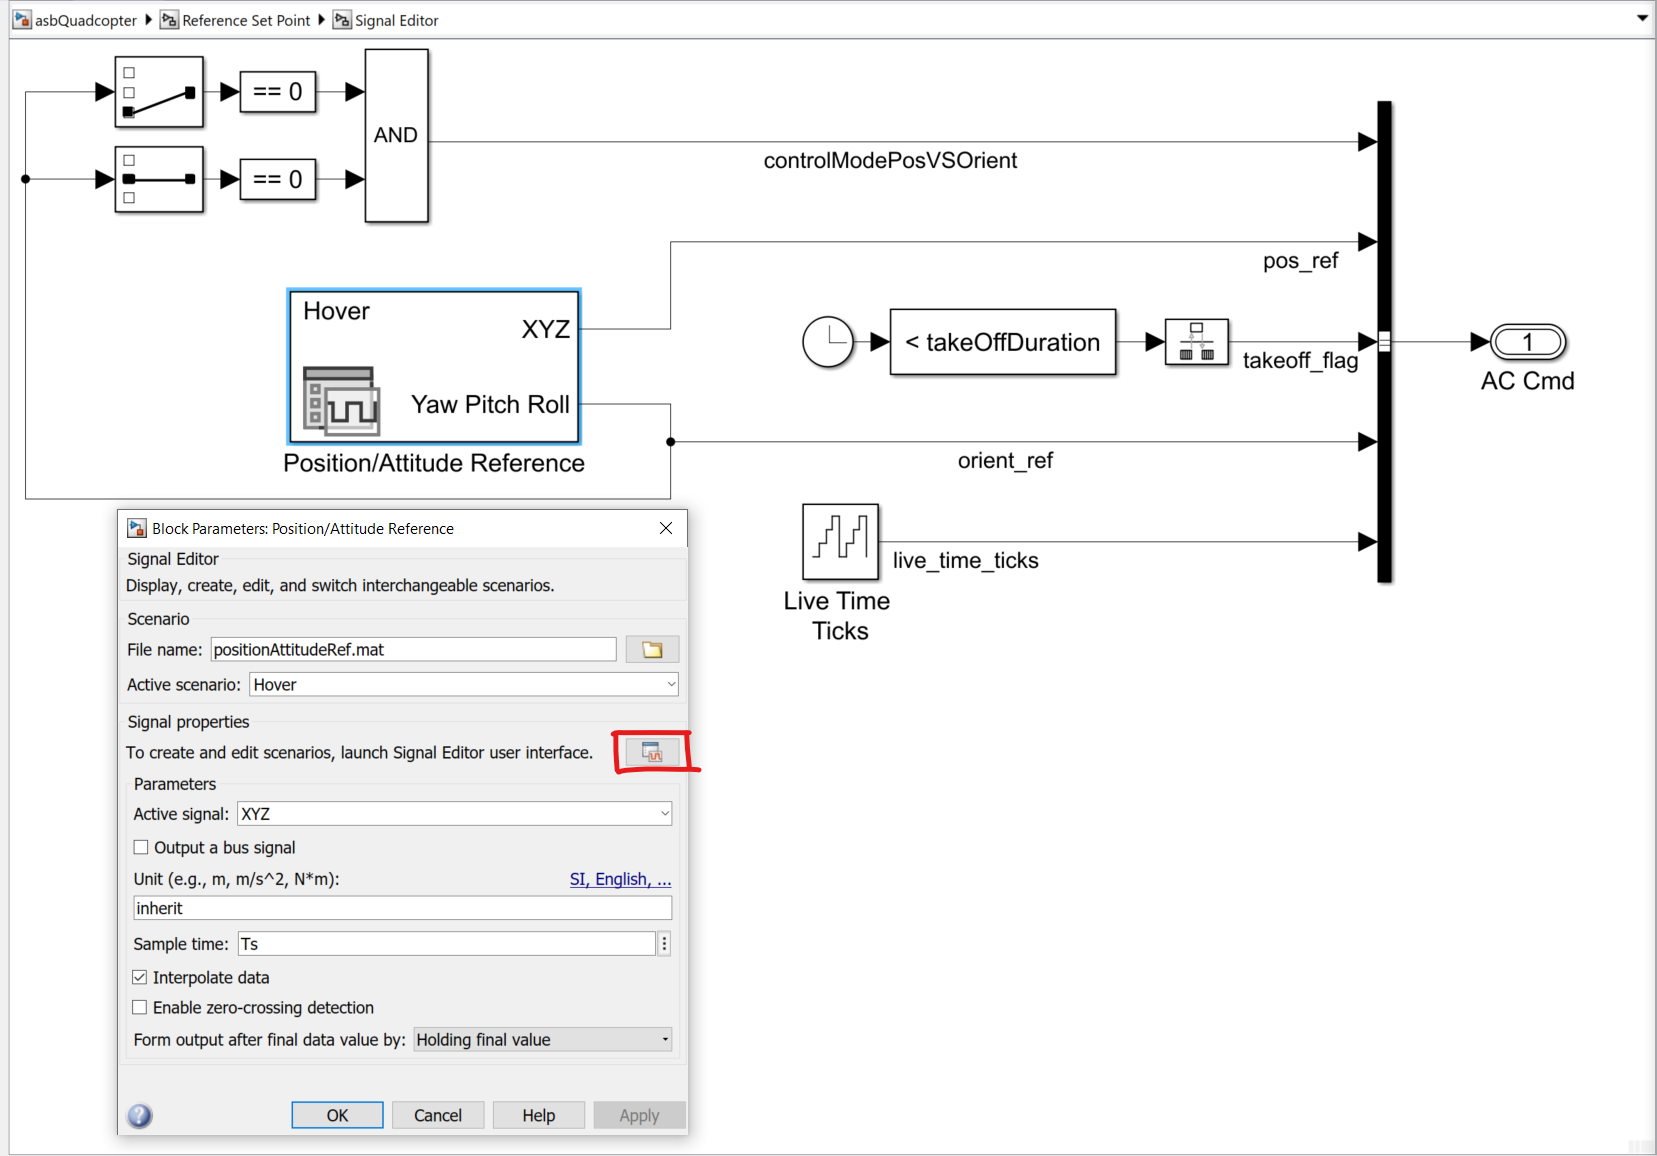
\includegraphics[width=1\textwidth]{signal-editor-open.png}
	\caption{Como abrir o Editor de Sinais}
	\centering
	\label{sinal-editor-open}
\end{figure}

No editor de sinais, podemos inserir nossos dados de entrada, para os nossos seis graus de liberdade, e em qual momento da simulação o sinal será enviado.


\begin{figure}[H]
	\centering
	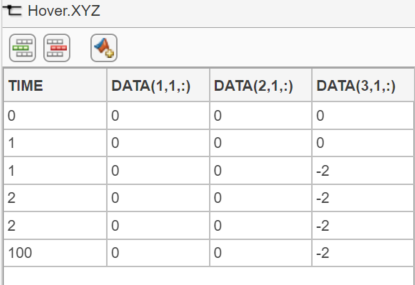
\includegraphics[width=1\textwidth]{signal-editor-xyz-hover.png}
	\caption{Modificando cenários de Simulação X Y Z}
	\centering
	\label{sinal-editor-xyz-hover}
\end{figure}

\begin{figure}[H]
	\centering
	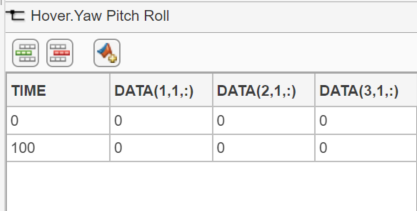
\includegraphics[width=1\textwidth]{signal-editor-pry-hover.png}
	\caption{Modificando cenários de Simulação Guinada, Arfagem e Rolagem}
	\centering
	\label{signal-editor-pry-hover}
\end{figure}


Para executar os cenários de forma programática e pegar os resultados, utilizaremos um código retirado também da nossa principal referência nesse capítulo.

\begin{lstlisting}[language=Matlab, caption={Configuração de Cenários no MATLAB Simulink}]
	scenarios = {'TesteXY3'; 'LandingSearch'};
	TFinals = [25;30];
	
	in = Simulink.SimulationInput.empty(size(scenarios, 1), 0);
	for i = 1 : size(scenarios, 1)
		in(i) = Simulink.SimulationInput('asbQuadcopter');
		in(i) = in(i).setBlockParameter(['flightControlSystem/Flight Control System/' ...
			'landing logic/Position//Attitude Reference'], ...
			'ActiveScenario', scenarios{i});
		in(i) = in(i).setVariable('TFinal', TFinals(i), 'Workspace', 'asbQuadcopter');
	end
	
	out = sim(in(1)); % simulate with the "Hover" scenario for 10 seconds
\end{lstlisting}

No código acima, as linhas 1 e 2 definem o cenário que pretendemos simular(previamente criado dentro do editor de sinais), e o tempo de simulação, respectivamente. O laço de repetição da linha 5 a 11, coloca o cenário no bloco Position/Attitude Reference que está dentro de \textit{Landing logic}, que foi inserido após as modificações que seguimos na seção \textit{configuraçôes de entrada}. A linha 13, executa a simulação com o cenário escolhido e salva os resultados na variável \textit{out}.

A variável \textit{out}, contém todas as informações que são do nosso interesse, no seguinte formato:

\begin{lstlisting}[language=Matlab, caption={Exemplo de extração de dados simulados}, numbers=left, backgroundcolor=\color{lightgray}]
	t = out.posref.time;
	xyzrpy = out.xyzrpy;
	estim = out.estim.signals.values;
	posref = out.posref.signals.values;
	motor = out.motor.signals.values;
	sensor = out.sensor.signals.values;
\end{lstlisting}

Com isso, agora podemos executar os cenários com facilidade e colocar os resultados de forma gráfica, para observamos o comportamento dos controladores.

\subsection{Resultados}

Nesta seção, será realizada a análise dos gráficos gerados a partir das simulações realizadas no MATLAB Simulink. O objetivo principal é avaliar o desempenho dos controladores do quadricóptero em diferentes cenários, com foco no comportamento das variáveis de interesse, como a posição \(x\), \(y\), \(z\) e os ângulos de rolagem, arfagem e guinada.

Para interpretar os gráficos de desempenho, serão consideradas as seguintes métricas:
\begin{itemize}
    \item \textbf{Tempo de estabilização}: Tempo necessário para que o sistema se estabilize após uma mudança de referência ou perturbação.
    \item \textbf{Overshoot (ultrapassagem)}: A porcentagem que a resposta do sistema excede o valor de referência antes de se estabilizar.
    \item \textbf{Erro em regime permanente}: A diferença entre o valor final da variável controlada e o valor de referência após o sistema estabilizar.
    \item \textbf{Tempo de subida}: O tempo que o sistema leva para sair de 10\% a 90\% do valor final após uma mudança de referência.
\end{itemize}

Essas métricas permitirão avaliar a eficácia dos controladores em manter o quadricóptero estável e responsivo, principalmente no cenário de voo pairado (\textit{Hover}), onde a precisão de posição e estabilidade são cruciais.

Os gráficos apresentam o comportamento das coordenadas do quadricóptero ao longo do tempo nos cenários de interesse montados. Ele compara três curvas: \textbf{Posição verdadeiro} (linha azul), que representa a altura real do quadricóptero; \textbf{Posição estimado} (linha laranja), que é a estimativa feita pelo sistema; e \textbf{Posição referência} (linha amarela), que é o valor de referência.

Nas curvas de atitude, é necessário elucidar melhor os termos os termos utilizados. Assim, aqui é preciso lembrar que para o quadricóptero realizar movimentos horinzontais, é necessário que aconteça uma arfagem ou rolagem, e no controlador de voo, temos um subsistema que converte os valore de de referência de x e y, em comandos de rolagem e arfagem. Nos gráficos, a resultande desses valores são chamados de  \textbf{comando de arfagem} e \textbf{comando de rolagem}.

\subsubsection{Voo Pairado (Hover)}

Neste cenário de voo pairado, o objetivo é que o drone suba até uma altura determinada e permaneça nessa altura até o fim da simulação. Além de analisar o desempenho do controlador de altitude, é interessante observar o comportamento dos controladores de posição nos eixos \(X\) e \(Y\), além dos controladores de arfagem, guinada e rolagem.

Parâmetros da simulação: \\

- Tempo total: 25 segundos;\\
- Altura desejada: 2 metros; \\
- Posição em \(X\) e \(Y\): 0.

1) Coordenada Z

\begin{figure}[H]
	\centering
	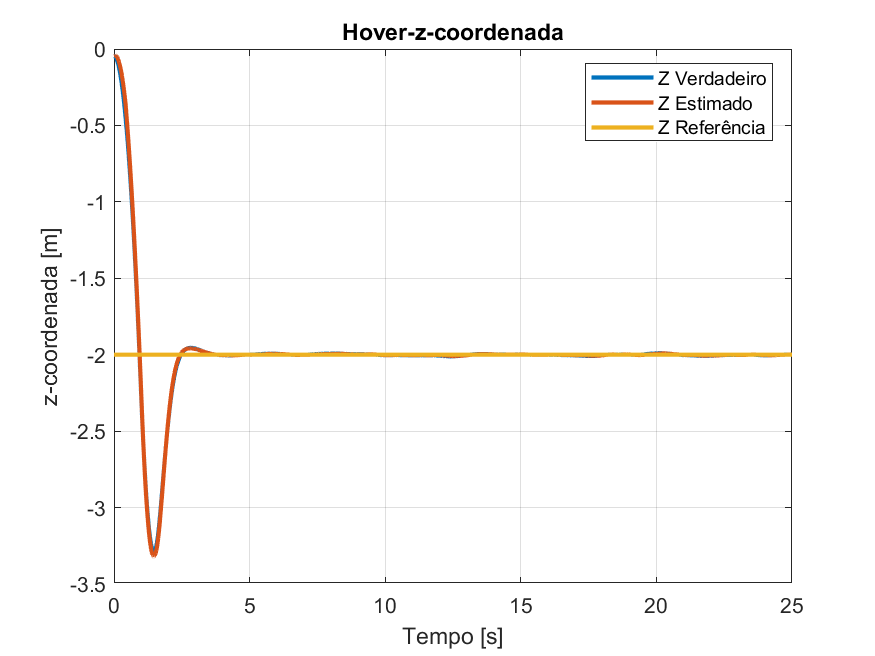
\includegraphics[width=1\textwidth]{Hover-z-coordenada.png}
	\caption{Coordenada Z para o Cenário de Voo Pairado}
	\label{fig:hover-z-coordenada}
\end{figure}

Analisando o gráfico, podemos observar que o tempo de estabilização é rápido, por volta dos 3 segundos, após o qual o sistema atinge a estabilidade próximo ao valor de referência. Um pequeno overshoot é visível no início, mas é bem controlado, e o erro em regime permanente é mínimo, indicando um bom desempenho do controlador para manter a altitude.

2) Coordenadas X e Y

Abaixo estão os gráficos das coordenadas \(X\) e \(Y\) do quadricóptero ao longo do tempo:

\begin{figure}[htbp]
    \centering
    \subfloat[Coordenada X para o Cenário de Voo Pairado]{
        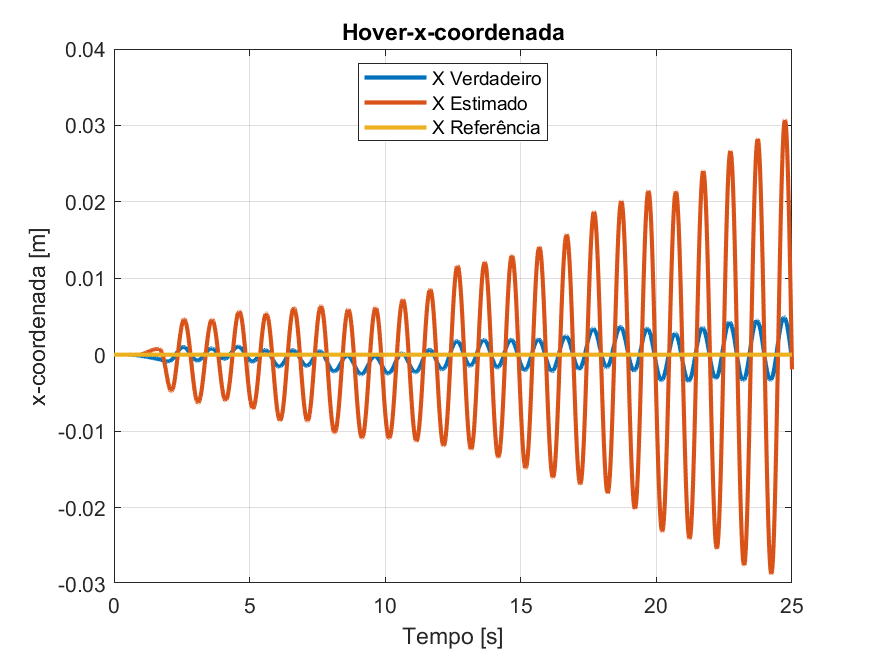
\includegraphics[width=0.45\textwidth]{Hover-x-coordenada.png}
        \label{fig:hover-x-coordenada}
    }
    \hfill
    \subfloat[Coordenada Y para o Cenário de Voo Pairado]{
        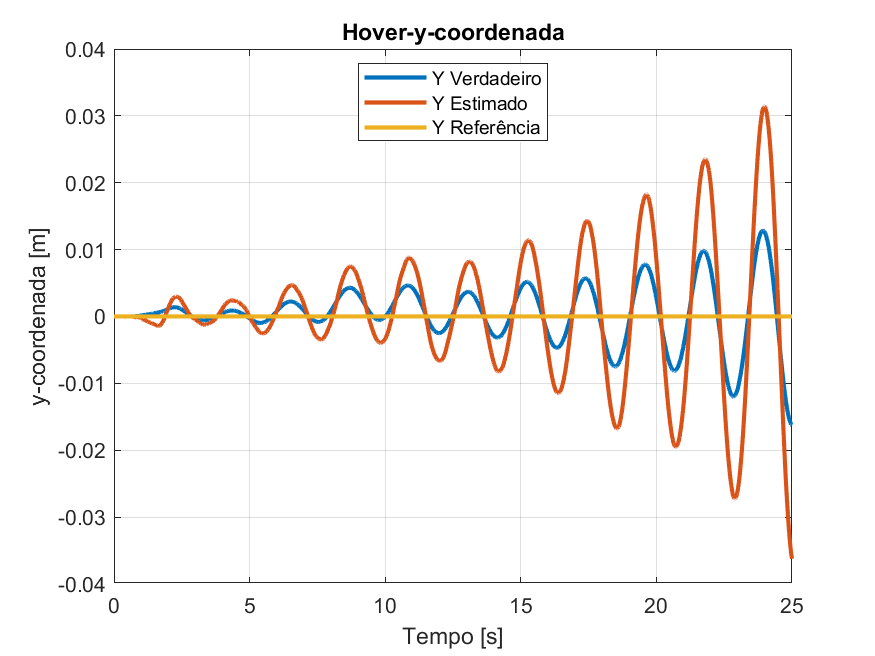
\includegraphics[width=0.45\textwidth]{Hover-y-coordenada.png}
        \label{fig:hover-y-coordenada}
    }
    \caption{Coordenadas X e Y para o Cenário de Voo Pairado}
    \label{fig:hover-x-y-coordenadas}
\end{figure}

No dois gráficos, podemos observar oscilações crescentes em torno do valor de referência com o tempo. No gráfico do eixo \(Y\), vemos que o valor verdadeiro aumenta ao longo do tempo proporcionalmente com os valores estimados, na curva de \(X\), apesar das altas oscilações dos valores estimados, o valor verdadeiro consegue se manter próximo ao valor de referência.

%Para ambos os eixos, uma possível solução é ajustar os ganhos \(K_p\) e \(K_d\) para suavizar a resposta e aumentar o amortecimento, além de adicionar um ganho integral \(K_i\) para reduzir o erro em regime permanente.

3) Ângulos de Rolagem, Arfagem e Guinada

A seguir estão os gráficos para os ângulos de rotação do quadricóptero: rolamento (roll), arfagem (pitch) e guinada (yaw).

\begin{figure}[htbp]
    \centering
    \subfloat[Arfagem para o Cenário de Voo Pairado]{
        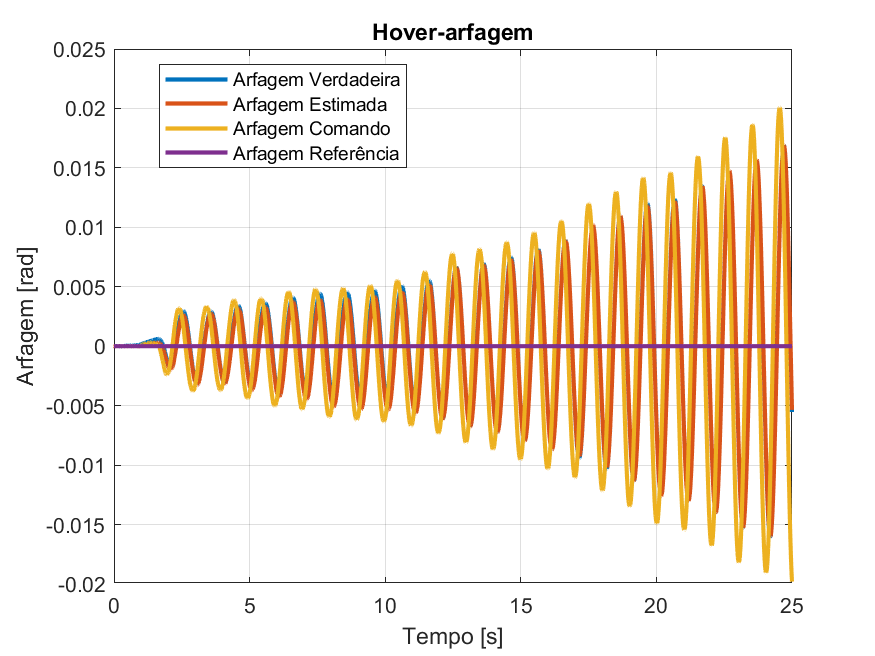
\includegraphics[width=0.45\textwidth]{Hover-arfagem.png}
        \label{fig:hover-arfagem}
    }
    \hfill
    \subfloat[Guinada para o Cenário de Voo Pairado]{
        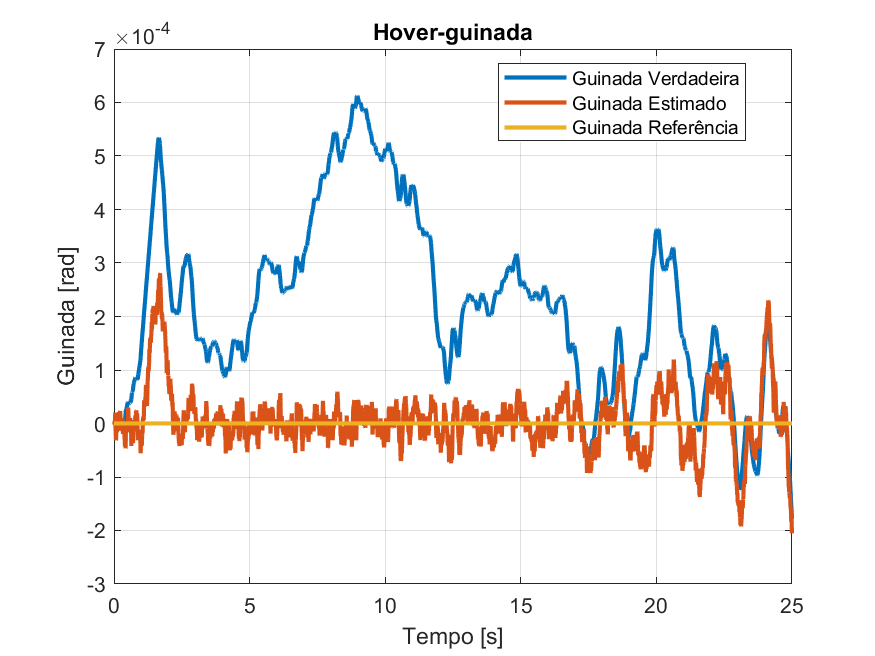
\includegraphics[width=0.45\textwidth]{Hover-guinada.png}
        \label{fig:hover-guinada}
    }
    \caption{Arfagem e Guinada para o Cenário de Voo Pairado}
    \label{fig:hover-arfagem-guinada}
\end{figure}

\begin{figure}[H]
	\centering
	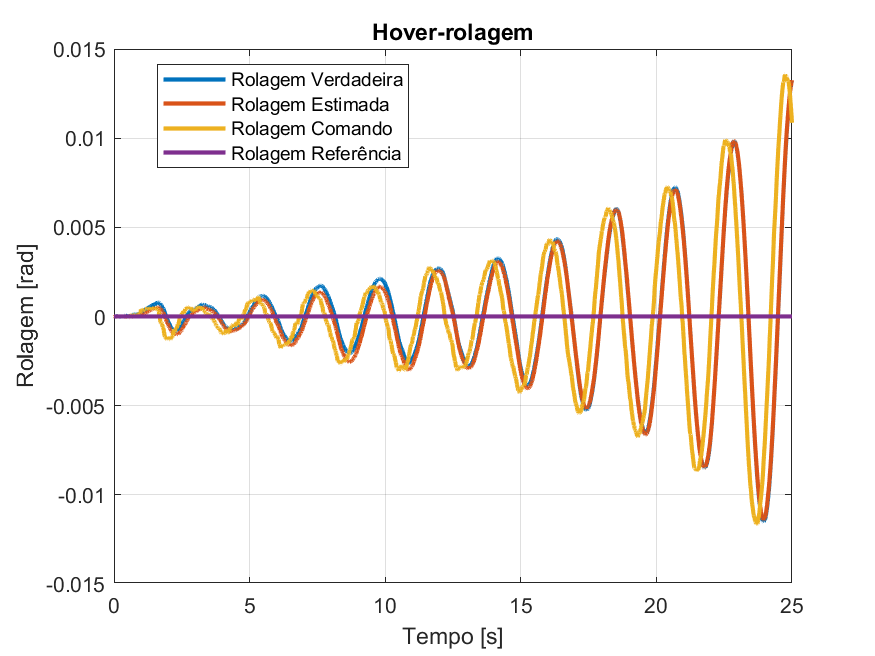
\includegraphics[width=0.5\textwidth]{Hover-rolagem.png}
	\caption{Rolagem para o Cenário de Voo Pairado}
	\label{fig:hover-rolagem}
\end{figure}

Nos gráficos, vemos que os ângulos de arfagem e rolamento apresentam oscilações crescentes ao longo do tempo, o que inclusive concorda com o comportamento que observamos nos eixos  \(X\) e  \(Y\) ,enquanto o ângulo de guinada permanece relativamente estável. Essas oscilações indicam uma possível falta de amortecimento no controlador, especialmente nos eixos de arfagem e rolamento.

Sendo assim, uma boa estratégia para iniciarmos nossas melhorias seria ajustar os parâmetros dos controladores de arfagem e rolagem, bem como os contralores da posição \(X\) e \(Y\).



%Para melhorar o desempenho, recomenda-se ajustar os parâmetros do controlador para reduzir as oscilações nesses eixos, aplicando amortecimento adicional e revisando os ganhos de controle. Isso deve resultar em um sistema mais estável e menos propenso a oscilações crescentes.

%Conclusão Geral para o Cenário de Voo Pairado

%No cenário de voo pairado, o controlador de altitude apresenta um bom desempenho, mas os controladores de posição e atitude nos eixos \(X\) e \(Y\), assim como os controladores de rotação (roll e pitch), mostram sinais de instabilidade. Ajustes nos parâmetros de controle são recomendados para melhorar a resposta geral e a estabilidade do sistema, especialmente em situações que exigem controle preciso de posição e orientação.




%---------------------------------------------------------------------
% INDICE REMISSIVO
%---------------------------------------------------------------------
\phantompart
\printindex
%---------------------------------------------------------------------

%\subsubsection{Mudança de Altitude (Altitude Change)}

Neste cenário de mudança de altitude, o objetivo é que o drone ajuste sua altura em resposta a uma nova referência de altitude, mantendo-se estável nas posições \(X\) e \(Y\) durante essa mudança. Além de analisar o desempenho do controlador de altitude, também é importante observar como os controladores de posição e atitude reagem a essa transição.

Parâmetros da simulação: \\

- Tempo total: 25 segundos;\\
- Altura inicial: 2 metros; \\
- Altura desejada: 1 metros; \\
- Posição em \(X\) e \(Y\): 0, 0. \\
- t mudança de altitude: 2s



1) Coordenada Z

O gráfico abaixo mostra o comportamento da coordenada \(Z\) ao longo do tempo.

\begin{figure}[H]
	\centering
	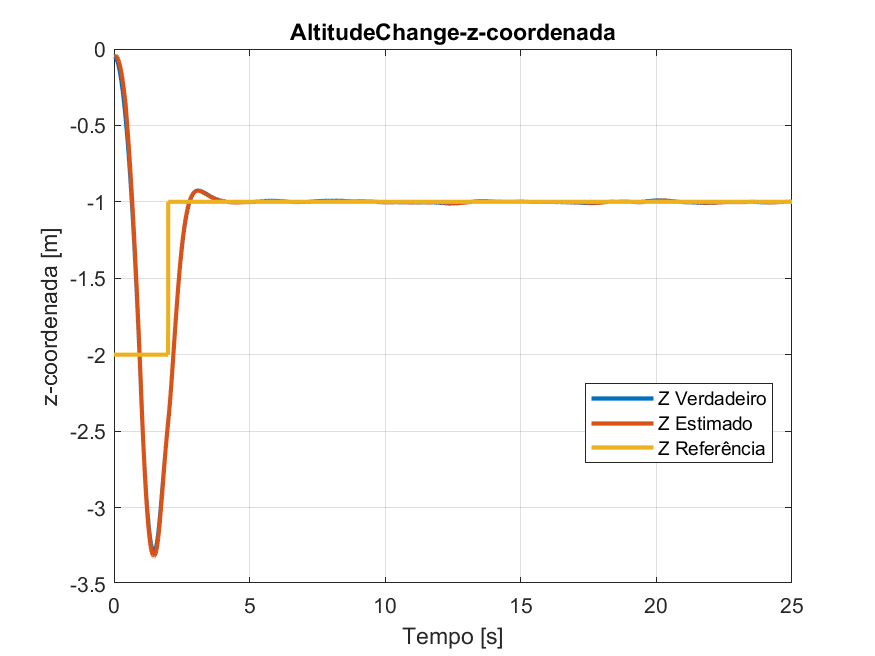
\includegraphics[width=1\textwidth]{AltitudeChange-z-coordenada.png}
	\caption{Coordenada Z para o Cenário de Mudança de Altitude}
	\label{fig:altitudechange-z-coordenada}
\end{figure}

Observamos que o sistema atinge a nova referência de altitude rapidamente, com um pequeno overshoot após a mudança de altitude. A estabilização ocorre após aproximadamente 5 segundos. Esse comportamento indica um bom desempenho do controlador de altitude para alcançar o valor de referência com um erro em regime permanente praticamente nulo.

2) Coordenadas X e Y

Os gráficos a seguir mostram o comportamento das coordenadas \(X\) e \(Y\) ao longo do tempo, permitindo uma análise do controle de posição durante a mudança de altitude.

\begin{figure}[htbp]
    \centering
    \subfloat[Coordenada X para o Cenário de Mudança de Altitude]{
        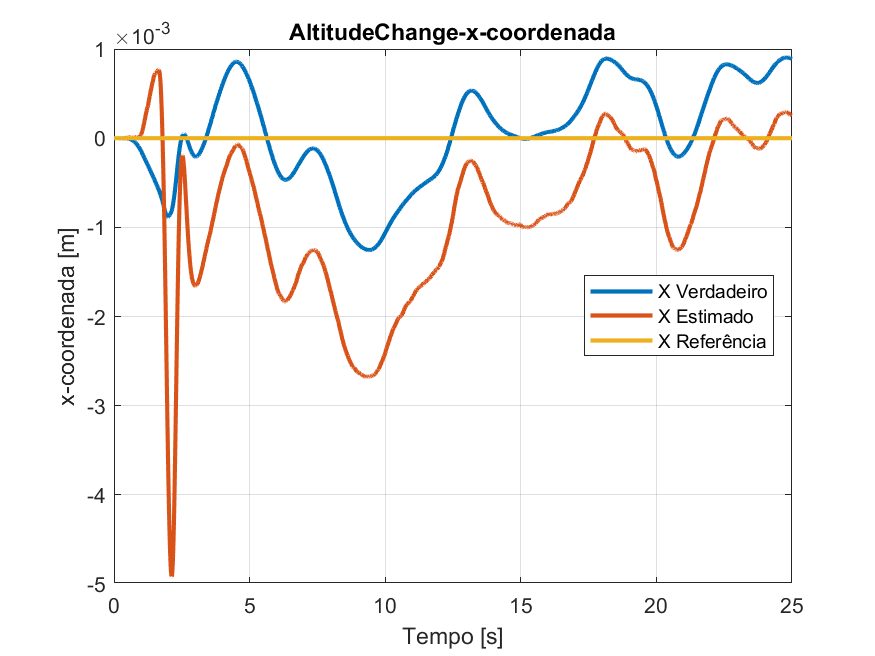
\includegraphics[width=0.45\textwidth]{AltitudeChange-x-coordenada.png}
        \label{fig:altitudechange-x-coordenada}
    }
    \hfill
    \subfloat[Coordenada Y para o Cenário de Mudança de Altitude]{
        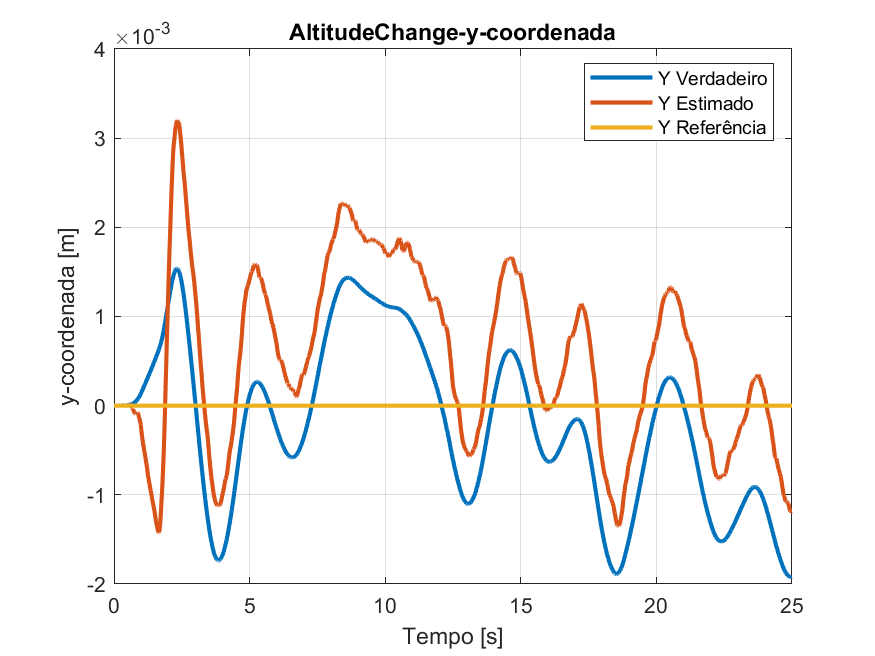
\includegraphics[width=0.45\textwidth]{AltitudeChange-y-coordenada.png}
        \label{fig:altitudechange-y-coordenada}
    }
    \caption{Coordenadas X e Y para o Cenário de Mudança de Altitude}
    \label{fig:altitudechange-x-y-coordenadas}
\end{figure}

Nos gráficos das coordenadas \(X\) e \(Y\), observamos que, durante a mudança de altitude, as posições \(X\) e \(Y\) nâo exibem oscilações significativas, na ordem dos milímetros, em torno da posição de referência. A curva de estimativa de posição \(Y\) (linha laranja) tem uma amplitude de oscilação baixa em comparação com a curva verdadeira e podemos ver que a amplitiude diminui com o tempo. No gráfico de \(X\), o comportamento é semelhante, com oscilações que diminuem progressivamente em direção a estabilidade.

Essas oscilações mostran que o sistema de controle de posição consegue manter a estabilidade durante a transição de altitude. Sendo interessante notar que o sistema de comporta melhor após a mudança de altitude do que num voo pairado, sendo assim, ao realizar nossos ajustes no sistema para melhorar o desempenho em voo pairado, devemos tomar cuidado para não prejudicar o sistema em um cenário de mudança de altitude..

3) Ângulos de Rolagem, Arfagem e Guinada

Os gráficos a seguir mostram os ângulos de rolamento (roll), arfagem (pitch) e guinada (yaw) do quadricóptero durante a mudança de altitude.

\begin{figure}[htbp]
    \centering
    \subfloat[Arfagem para o Cenário de Mudança de Altitude]{
        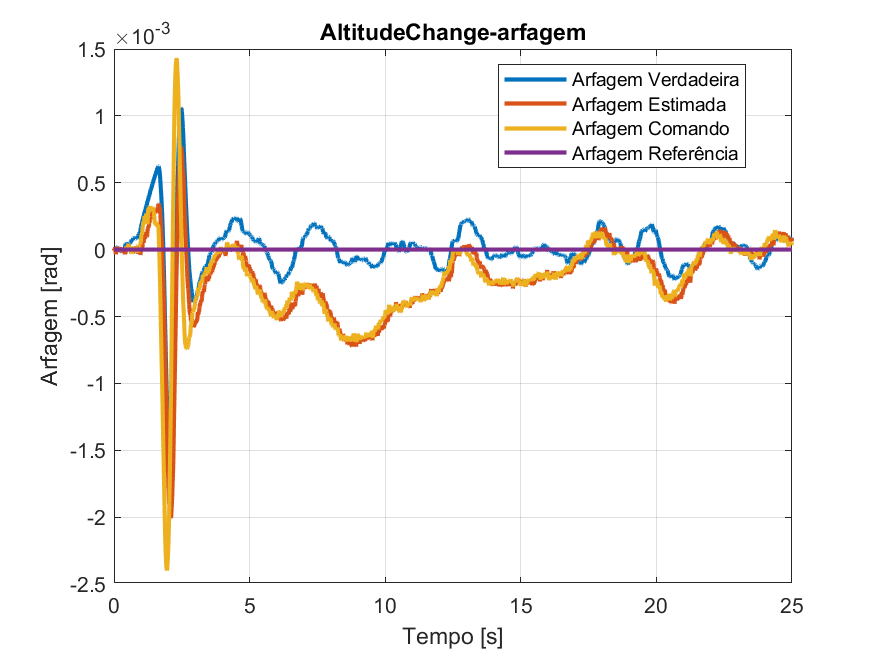
\includegraphics[width=0.45\textwidth]{AltitudeChange-arfagem.png}
        \label{fig:altitudechange-arfagem}
    }
    \hfill
    \subfloat[Guinada para o Cenário de Mudança de Altitude]{
        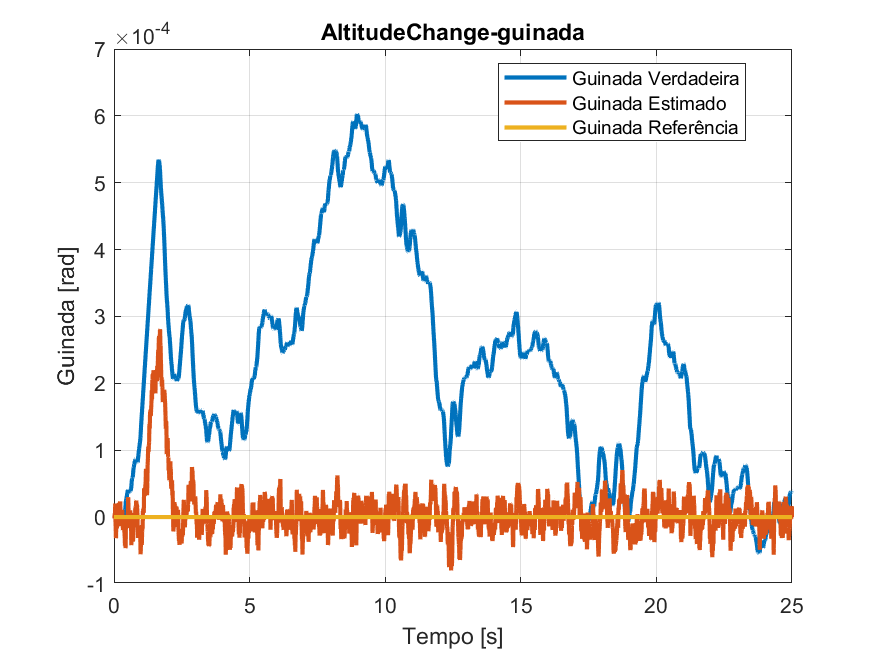
\includegraphics[width=0.45\textwidth]{AltitudeChange-guinada.png}
        \label{fig:altitudechange-guinada}
    }
    \caption{Arfagem e Guinada para o Cenário de Mudança de Altitude}
    \label{fig:altitudechange-arfagem-guinada}
\end{figure}

\begin{figure}[H]
	\centering
	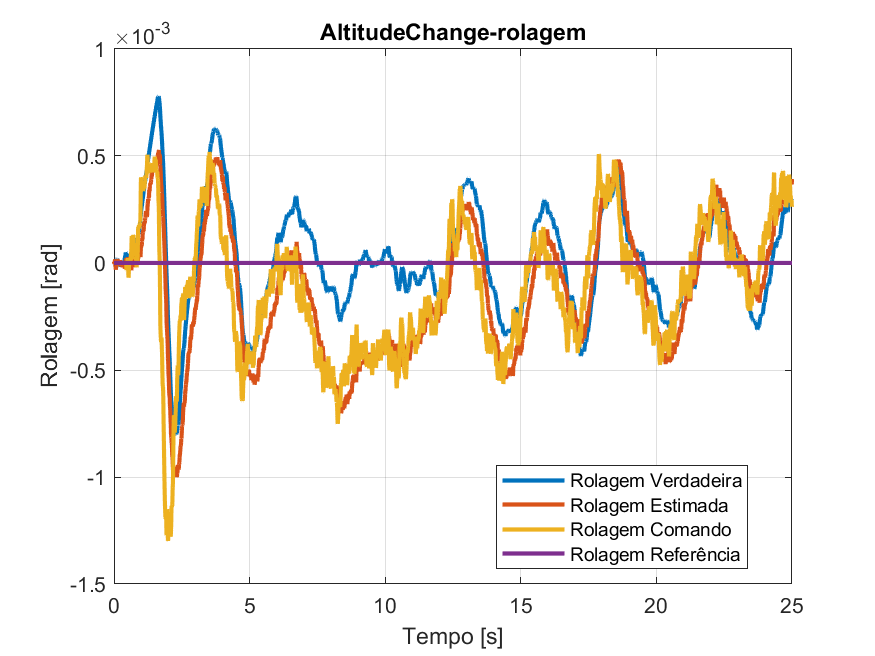
\includegraphics[width=0.5\textwidth]{AltitudeChange-rolagem.png}
	\caption{Rolagem para o Cenário de Mudança de Altitude}
	\label{fig:altitudechange-rolagem}
\end{figure}

Durante a transição de altitude, os ângulos de arfagem e rolamento apresentam oscilações notáveis, mas de baixa amplitude. No gráfico de arfagem e de rolagem, observa-se um comportamento oscilatório acentuado no momento da mudança de altitude,mas que com o tempo tende a estabilidade em torno do valor de referência, o que indica que o controlador precisa ser ajustado para responder de forma mais suave. O gráfico de guinada mostra variações menores, o que sugere um controle mais estável para esse eixo.

%A amplitude das oscilações em rolamento e arfagem indica que o sistema de controle está mal ajustado para esses eixos durante a transição de altitude. Ajustes nos parâmetros de controle, como o ganho derivativo \(K_d\), poderiam ajudar a reduzir essas oscilações e melhorar a resposta do sistema.

%### Conclusão Geral para o Cenário de Mudança de Altitude

%No cenário de mudança de altitude, o controlador de altitude funciona bem, atingindo o novo valor de referência de forma rápida e com mínimo erro em regime permanente. No entanto, os controladores de posição nos eixos \(X\) e \(Y\) e os controladores de atitude nos eixos de rolamento e arfagem exibem sinais de instabilidade, com oscilações crescentes ao longo do tempo. Para melhorar o desempenho, recomenda-se um ajuste nos ganhos do controlador, especialmente nos eixos \(X\) e \(Y\), bem como nos controladores de atitude, para reduzir as oscilações e melhorar a estabilidade geral do sistema.


%---------------------------------------------------------------------
% INDICE REMISSIVO
%---------------------------------------------------------------------
\phantompart
\printindex
%---------------------------------------------------------------------

%\subsubsection{Altidude Constante seguido de Arfagem}

Neste cenário, o objetivo é que o quadricóptero mantenha uma atitude fixa em arfagem (\textit{pitch}) enquanto estabiliza a altitude e as posições \(X\) e \(Y\). A análise considera a resposta dos controladores para cada uma dessas variáveis, observando-se as trajetórias real, estimada e de referência.

Parâmetros da simulação: \\

- Tempo total: 30 segundos;\\
- Altura desejada: 2 metros; \\
- Arfagem de 0.1 rad(5,73 graus) em t =5s

1) Arfagem

O gráfico a seguir mostra o comportamento do ângulo de arfagem ao longo do tempo.

\begin{figure}[H]
	\centering
	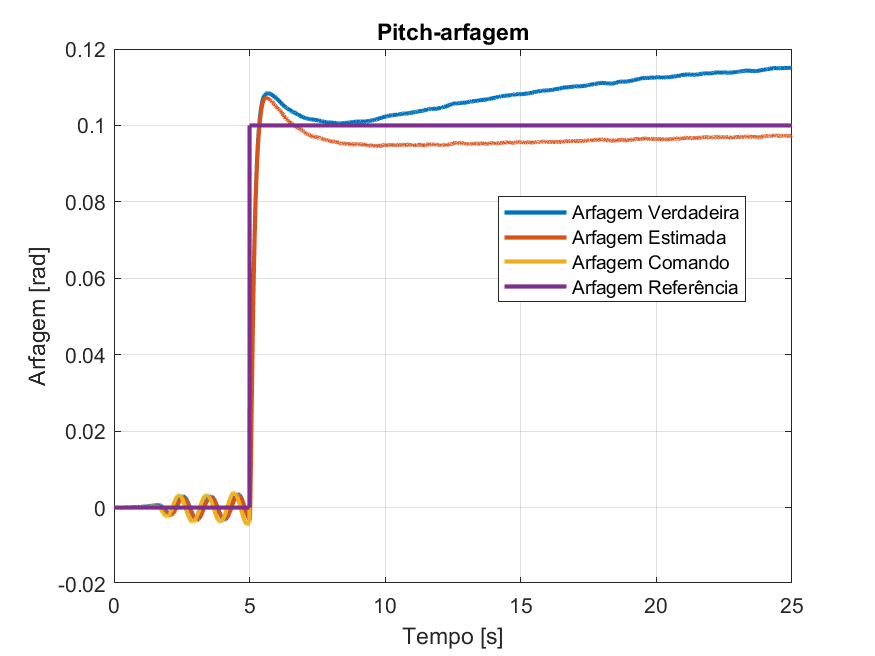
\includegraphics[width=0.8\textwidth]{Pitch-arfagem.png}
	\caption{Arfagem para o Cenário de Pitch}
	\label{fig:pitch-arfagem}
\end{figure}

Neste gráfico, observamos que o ângulo de arfagem responde rapidamente ao comando de referência, alcançando um valor de aproximadamente \(0.1\) radianos. Contudo, notamos uma pequena diferença entre a curva verdadeira (linha azul) e a estimada (linha laranja) após a arfagem. Essa diferença indica uma leve defasagem entre o valor verdadeiro e o valor estimado. A curva de referência (linha roxa) permanece constante, indicando o ângulo alvo desejado para este cenário.

2) Coordenada X

A seguir, temos o gráfico da posição \(X\) do quadricóptero ao longo do tempo.

\begin{figure}[H]
	\centering
	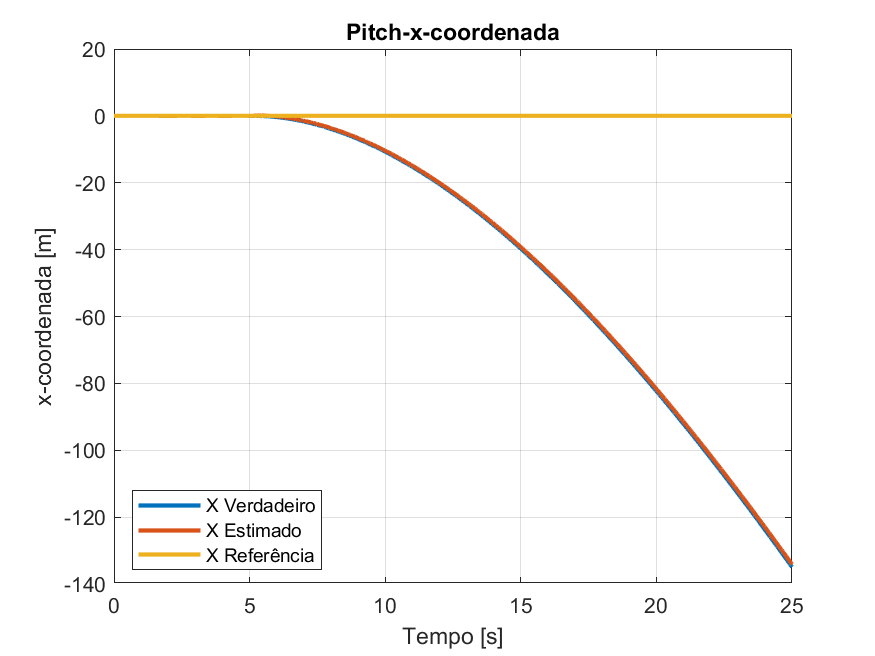
\includegraphics[width=0.8\textwidth]{Pitch-x-coordenada.png}
	\caption{Coordenada X para o Cenário de Pitch}
	\label{fig:pitch-x-coordenada}
\end{figure}

A posição \(X\) mostra um comportamento de translação contínua ao longo do tempo, conforme esperado para um cenário de arfagem constante, onde o quadricóptero se desloca em direção ao eixo \(X\). As curvas verdadeira e estimada (linhas azul e laranja) coincidem bem, indicando uma boa precisão na estimativa de posição.

3) Coordenada Z

Por fim, analisamos o comportamento da coordenada \(Z\) ao longo do tempo.

\begin{figure}[H]
	\centering
	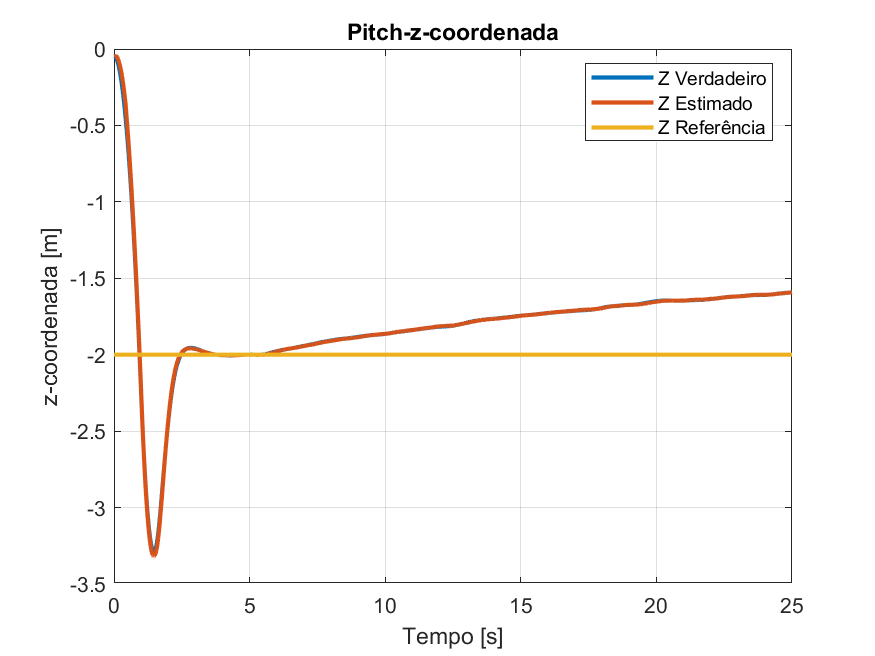
\includegraphics[width=0.8\textwidth]{Pitch-z-coordenada.png}
	\caption{Coordenada Z para o Cenário de Pitch}
	\label{fig:pitch-z-coordenada}
\end{figure}

Neste gráfico, a altitude mostra uma leve tendência de aumento com o passar do tempo, ainda que a referência de altura permaneça constante. A diferença entre as curvas verdadeira e estimada mostra que o sistema de controle está encontrando dificuldade para manter a altitude estável quando a inclinação de pitch é aplicada.

%### Conclusão Geral para o Cenário de Pitch

%O cenário de pitch revela um bom desempenho na estimativa de posição \(X\) e \(Y\), com ambas as curvas de posição verdadeira e estimada acompanhando bem a referência ao longo do tempo. No entanto, o controle de altitude apresenta uma leve instabilidade, o que pode exigir ajustes nos parâmetros do controlador para evitar desvios indesejados na coordenada \(Z\). Além disso, a leve diferença entre as curvas de arfagem verdadeira e estimada sugere que ajustes no controlador de pitch poderiam melhorar ainda mais a precisão da resposta do sistema.


%---------------------------------------------------------------------
% INDICE REMISSIVO
%---------------------------------------------------------------------
\phantompart
\printindex
%---------------------------------------------------------------------

%\subsubsection{Altidude Constante seguido de Rolagem}

Neste cenário, o objetivo é que o quadricóptero mantenha uma atitude fixa em arfagem (\textit{pitch}) enquanto estabiliza a altitude e as posições \(X\) e \(Y\). A análise considera a resposta dos controladores para cada uma dessas variáveis, observando-se as trajetórias real, estimada e de referência.

Parâmetros da simulação: \\

- Tempo total: 30 segundos;\\
- Altura desejada: 2 metros; \\
- Rolagem de 0.1 rad(5,73 graus) em t =5s

1) Rolagem

O gráfico a seguir mostra o comportamento do ângulo de arfagem ao longo do tempo.

\begin{figure}[H]
	\centering
	\includegraphics[width=0.8\textwidth]{Roll-rolagem.png}
	\caption{Rolagem para o Cenário de rolagem}
	\label{fig:roll-arfagem}
\end{figure}

Neste gráfico, observamos que o ângulo de arfagem responde rapidamente ao comando de referência, alcançando um valor de aproximadamente \(0.1\) radianos. Contudo, notamos uma pequena diferença entre a curva verdadeira (linha azul) e a estimada (linha laranja) após a rolagem. Essa diferença indica uma leve defasagem entre o valor verdadeiro e o valor estimado. A curva de referência (linha roxa) permanece constante, indicando o ângulo alvo desejado para este cenário.

2) Coordenada Y

A seguir, temos o gráfico da posição \(Y\) do quadricóptero ao longo do tempo.

\begin{figure}[H]
	\centering
	\includegraphics[width=0.8\textwidth]{Roll-y-coordenada.png}
	\caption{Coordenada Y para o Cenário de rolagem}
	\label{fig:roll-x-coordenada}
\end{figure}

A posição \(X\) mostra um comportamento de translação contínua ao longo do tempo, conforme esperado para um cenário de arfagem constante, onde o quadricóptero se desloca em direção ao eixo \(X\). As curvas verdadeira e estimada (linhas azul e laranja) coincidem bem, indicando uma boa precisão na estimativa de posição.

3) Coordenada Z

Por fim, analisamos o comportamento da coordenada \(Z\) ao longo do tempo.

\begin{figure}[H]
	\centering
	\includegraphics[width=0.8\textwidth]{roll-z-coordenada.png}
	\caption{Coordenada Z para o Cenário de Rolagem}
	\label{fig:roll-z-coordenada}
\end{figure}

Neste gráfico, a altitude mostra uma leve tendência de aumento com o passar do tempo, ainda que a referência de altura permaneça constante. A diferença entre as curvas verdadeira e estimada mostra que o sistema de controle está encontrando dificuldade para manter a altitude estável quando a inclinação de pitch é aplicada.

%### Conclusão Geral para o Cenário de Pitch

%O cenário de pitch revela um bom desempenho na estimativa de posição \(X\) e \(Y\), com ambas as curvas de posição verdadeira e estimada acompanhando bem a referência ao longo do tempo. No entanto, o controle de altitude apresenta uma leve instabilidade, o que pode exigir ajustes nos parâmetros do controlador para evitar desvios indesejados na coordenada \(Z\). Além disso, a leve diferença entre as curvas de arfagem verdadeira e estimada sugere que ajustes no controlador de pitch poderiam melhorar ainda mais a precisão da resposta do sistema.


%---------------------------------------------------------------------
% INDICE REMISSIVO
%---------------------------------------------------------------------
\phantompart
\printindex
%---------------------------------------------------------------------


%---------------------------------------------------------------------
% INDICE REMISSIVO
%---------------------------------------------------------------------
\phantompart
\printindex
%---------------------------------------------------------------------




%\section{Análise do Cenário PitchRoll}

Neste cenário, o quadricóptero foi submetido a um comando de pitch seguido de um comando de roll, onde avaliamos as respostas nas coordenadas de arfagem, guinada, rolagem e nas coordenadas \(x\), \(y\) e \(z\).

\subsection{Arfagem}

\begin{figure}[H]
    \centering
    \includegraphics[width=0.7\textwidth]{PitchRoll-arfagem.png}
    \caption{Resposta em Arfagem para o cenário Pitch seguido de Roll}
    \label{fig:pitchroll-arfagem}
\end{figure}

No gráfico da Figura \ref{fig:pitchroll-arfagem}, observamos que, após o comando inicial de pitch, o sistema rapidamente se ajusta, mas, ao adicionar o comando de roll, ocorre uma oscilação significativa. Esse comportamento sugere uma leve instabilidade momentânea ao alternar entre os dois comandos. A diferença entre a curva estimada e a verdadeira também se torna mais evidente após o comando de roll, indicando a necessidade de ajustes nos parâmetros do controlador para uma resposta mais uniforme e próxima da referência.

\subsection{Guinada}

\begin{figure}[H]
    \centering
    \includegraphics[width=0.7\textwidth]{PitchRoll-guinada.png}
    \caption{Resposta em Guinada para o cenário Pitch seguido de Roll}
    \label{fig:pitchroll-guinada}
\end{figure}

Na Figura \ref{fig:pitchroll-guinada}, notamos uma oscilação acentuada na guinada, especialmente após o comando de roll. A curva verdadeira apresenta uma amplitude significativamente maior do que a curva estimada, o que indica que o controlador está tendo dificuldade em amortecer as oscilações na guinada durante as mudanças de atitude. Isso sugere que o sistema pode estar subamortecido para este eixo, e um aumento no ganho derivativo pode ajudar a reduzir essa instabilidade.

\subsection{Rolagem}

\begin{figure}[H]
    \centering
    \includegraphics[width=0.7\textwidth]{PitchRoll-rolagem.png}
    \caption{Resposta em Rolagem para o cenário Pitch seguido de Roll}
    \label{fig:pitchroll-rolagem}
\end{figure}

A Figura \ref{fig:pitchroll-rolagem} mostra que, com a introdução do comando de roll, a resposta do sistema apresenta uma oscilação rápida e estabiliza, embora com uma leve diferença entre o valor verdadeiro e o estimado. A resposta geral sugere que o controlador de rolagem é eficaz em manter o controle, mas ajustes finos podem melhorar a precisão entre a resposta verdadeira e a estimada.

\subsection{Coordenadas X, Y e Z}

\begin{figure}[H]
    \centering
    \includegraphics[width=0.45\textwidth]{PitchRoll-x-coordenada.png}
    \includegraphics[width=0.45\textwidth]{PitchRoll-y-coordenada.png}
    \caption{Resposta nas coordenadas X e Y para o cenário Pitch seguido de Roll}
    \label{fig:pitchroll-xy-coordenadas}
\end{figure}

Nas Figuras \ref{fig:pitchroll-xy-coordenadas}, observamos que as coordenadas \(x\) e \(y\) sofrem uma mudança significativa, especialmente no eixo \(x\), onde o quadricóptero apresenta um movimento de deslocamento contínuo, o que reflete o impacto dos comandos de pitch e roll. A trajetória estimada acompanha a verdadeira, mas com um pequeno desvio. Esses desvios indicam que a estimativa de posição do sistema de controle precisa de ajustes para rastrear com maior precisão.

\begin{figure}[H]
    \centering
    \includegraphics[width=0.7\textwidth]{PitchRoll-z-coordenada.png}
    \caption{Resposta na coordenada Z para o cenário Pitch seguido de Roll}
    \label{fig:pitchroll-z-coordenada}
\end{figure}

Na Figura \ref{fig:pitchroll-z-coordenada}, a coordenada \(z\) apresenta uma leve oscilação após os comandos de pitch e roll, com uma tendência de subir ligeiramente após o segundo comando. Este comportamento indica que o controlador de altitude está reagindo aos comandos de pitch e roll com uma pequena alteração na altitude. Ajustes no controlador de altitude podem ser necessários para minimizar o impacto dessas oscilações.

%\subsection{Conclusão do Cenário PitchRoll}

%O cenário Pitch seguido de Roll evidencia que o sistema responde bem a comandos individuais de pitch e roll, mas apresenta desafios ao lidar com ambos simultaneamente, especialmente em relação à guinada e à estabilidade nas coordenadas \(x\) e \(y\). O controlador poderia ser aprimorado para lidar melhor com a combinação de comandos e minimizar o impacto em outros eixos, garantindo uma maior estabilidade e precisão.


%---------------------------------------------------------------------
% INDICE REMISSIVO
%---------------------------------------------------------------------
\phantompart
\printindex
%---------------------------------------------------------------------

%\subsubsection{Cenário Yaw}

Neste cenário, o objetivo é analisar o comportamento do controlador do quadricóptero ao ser submetido a uma mudança de guinada (yaw), enquanto os controladores dos outros eixos (pitch, roll e altitude) mantêm o quadricóptero estável em sua posição e altitude.

\begin{figure}[H]
    \centering
    \includegraphics[width=0.8\textwidth]{YAW-guinada.png}
    \caption{Resposta do Yaw para o Cenário de Mudança de Yaw}
    \label{fig:YAW-guinada}
\end{figure}

No gráfico da guinada (Figura \ref{fig:YAW-guinada}), observamos que o sistema responde rapidamente à mudança no ângulo de yaw, acompanhando a referência quase instantaneamente, com uma resposta sem oscilação significativa após a estabilização. A curva estimada (linha laranja) acompanha bem a referência (linha amarela), indicando que o controlador de yaw está bem ajustado para esse tipo de movimento.

\begin{figure}[H]
    \centering
    \includegraphics[width=0.8\textwidth]{YAW-arfagem.png}
    \caption{Resposta da Arfagem para o Cenário de Mudança de Yaw}
    \label{fig:YAW-arfagem}
\end{figure}

No gráfico da arfagem (Figura \ref{fig:YAW-arfagem}), é possível notar oscilações de pequena amplitude ao longo do tempo, mostrando uma leve oscilação residual como resposta à mudança de yaw. Essas oscilações indicam uma resposta cruzada mínima que não afeta significativamente a estabilidade geral do sistema.

\begin{figure}[H]
    \centering
    \includegraphics[width=0.8\textwidth]{YAW-rolagem.png}
    \caption{Resposta da Rolagem para o Cenário de Mudança de Yaw}
    \label{fig:YAW-rolagem}
\end{figure}

A resposta da rolagem (Figura \ref{fig:YAW-rolagem}) é semelhante à da arfagem, com oscilações leves que aumentam gradualmente, mas sem comprometimento da estabilidade do quadricóptero. Essas oscilações podem ser controladas com ajuste fino, caso necessário, mas o desempenho atual é satisfatório.

\begin{figure}[H]
    \centering
    \includegraphics[width=0.8\textwidth]{YAW-z-coordenada.png}
    \caption{Coordenada Z para o Cenário de Mudança de Yaw}
    \label{fig:YAW-z-coordenada}
\end{figure}

Na coordenada Z (Figura \ref{fig:YAW-z-coordenada}), observamos que o sistema mantém a altitude de forma estável, mesmo com a variação de yaw. O controlador de altitude parece ser robusto o suficiente para não ser afetado pelas mudanças no yaw.

\begin{figure}[H]
    \centering
    \includegraphics[width=0.8\textwidth]{YAW-y-coordenada.png}
    \caption{Coordenada Y para o Cenário de Mudança de Yaw}
    \label{fig:YAW-y-coordenada}
\end{figure}

A coordenada Y (Figura \ref{fig:YAW-y-coordenada}) apresenta um comportamento oscilatório leve, porém, devido à ação de yaw, o quadricóptero sofre pequenas variações de posição lateral. As oscilações são mínimas e não comprometem o controle de posição.

\begin{figure}[H]
    \centering
    \includegraphics[width=0.8\textwidth]{YAW-x-coordenada.png}
    \caption{Coordenada X para o Cenário de Mudança de Yaw}
    \label{fig:YAW-x-coordenada}
\end{figure}

Na coordenada X (Figura \ref{fig:YAW-x-coordenada}), é possível observar um comportamento oscilatório similar ao observado em Y. O controlador mantém a estabilidade geral, mas há uma pequena resposta oscilatória induzida pela mudança de yaw.

%\textbf{Conclusão:} A resposta do quadricóptero no cenário de yaw é adequada e apresenta uma boa estabilidade. Embora pequenas oscilações apareçam nos eixos X, Y e nas atitudes de arfagem e rolagem, o controlador de yaw responde de maneira rápida e eficiente à mudança de referência. As oscilações são mínimas e poderiam ser ajustadas com um tuning fino, mas o desempenho geral é satisfatório para o cenário de mudança de yaw.



%---------------------------------------------------------------------
% INDICE REMISSIVO
%---------------------------------------------------------------------
\phantompart
\printindex
%---------------------------------------------------------------------

%\subsubsection{Cenário com Vento em X (WindX)}

Neste cenário, o objetivo é analisar o comportamento do quadricóptero sob a influência de uma rajada de vento na direção \(X\). Essa análise permite observar como o sistema de controle lida com perturbações externas no eixo \(X\), tanto em termos de estabilidade quanto de capacidade de retornar à posição desejada.

\begin{figure}[H]
    \centering
    \includegraphics[width=1\textwidth]{WindX-guinada.png}
    \caption{Comportamento da Guinada sob Vento em X}
    \label{fig:WindX-guinada}
\end{figure}

A Figura \ref{fig:WindX-guinada} mostra a resposta da guinada do quadricóptero ao vento em \(X\). Observa-se que o ângulo de guinada real (\textbf{Guinada Verdadeira}) apresenta variações significativas, enquanto a guinada estimada se mantém próxima da referência, indicando uma tentativa de manter a orientação desejada. Esse comportamento sugere que o sistema de controle tenta corrigir as perturbações, mas enfrenta dificuldades em eliminar completamente os efeitos do vento.

\begin{figure}[H]
    \centering
    \includegraphics[width=1\textwidth]{WindX-arfagem.png}
    \caption{Comportamento da Arfagem sob Vento em X}
    \label{fig:WindX-arfagem}
\end{figure}

Na Figura \ref{fig:WindX-arfagem}, observa-se o ângulo de arfagem. As oscilações crescentes na arfagem verdadeira sugerem uma resposta oscilatória e instável do sistema ao longo do tempo, enquanto a arfagem estimada acompanha esse comportamento, mas não consegue eliminá-lo totalmente. Esse fenômeno indica que o controlador de arfagem é impactado significativamente pelo vento, possivelmente necessitando de ajustes nos ganhos para melhorar o amortecimento.

\begin{figure}[H]
    \centering
    \includegraphics[width=1\textwidth]{WindX-rolagem.png}
    \caption{Comportamento da Rolagem sob Vento em X}
    \label{fig:WindX-rolagem}
\end{figure}

A Figura \ref{fig:WindX-rolagem} exibe a rolagem. A resposta segue um padrão oscilatório semelhante ao observado na arfagem, com oscilações que aumentam progressivamente ao longo do tempo. Esse comportamento indica que a rolagem também é sensível às perturbações, e o sistema de controle apresenta dificuldades em amortecer essas oscilações.

\begin{figure}[H]
    \centering
    \includegraphics[width=1\textwidth]{WindX-z-coordenada.png}
    \caption{Comportamento da Coordenada Z sob Vento em X}
    \label{fig:WindX-z-coordenada}
\end{figure}

Na Figura \ref{fig:WindX-z-coordenada}, observa-se a resposta em \(Z\). A coordenada \(Z\) verdadeira e estimada se mantêm relativamente estáveis após um leve overshoot inicial, sugerindo que o controle de altitude não é diretamente afetado pela rajada de vento em \(X\).

\begin{figure}[H]
    \centering
    \includegraphics[width=0.45\textwidth]{WindX-y-coordenada.png}
    \hfill
    \includegraphics[width=0.45\textwidth]{WindX-x-coordenada.png}
    \caption{Comportamento das Coordenadas X e Y sob Vento em X}
    \label{fig:WindX-x-y-coordenada}
\end{figure}

As Figuras \ref{fig:WindX-x-y-coordenada} mostram as respostas em \(X\) e \(Y\). Em \(X\), o sistema apresenta uma resposta oscilatória crescente, indicando uma instabilidade em resposta ao vento. Em \(Y\), as oscilações são também visíveis, o que indica que a rajada de vento em \(X\) provoca um acoplamento indesejado nos eixos laterais, afetando a estabilidade geral do quadricóptero.

%\subsubsection*{Conclusão}

%A análise do cenário com vento em \(X\) evidencia que o sistema de controle do quadricóptero possui limitações ao lidar com perturbações externas. As respostas oscilatórias e instáveis nas coordenadas \(X\), \(Y\), e nos ângulos de arfagem e rolagem sugerem que ajustes no controlador são necessários, especialmente para melhorar o amortecimento e a resistência a perturbações. Uma recomendação seria aumentar o ganho derivativo (\(K_d\)) para tentar reduzir as oscilações e obter uma resposta mais estável.


%---------------------------------------------------------------------
% INDICE REMISSIVO
%---------------------------------------------------------------------
\phantompart
\printindex
%---------------------------------------------------------------------

%\section{Análise do Cenário com Vento na Direção Y}

No cenário de vento na direção Y, analisamos as respostas dos ângulos de guinada, arfagem, e rolagem, bem como as coordenadas \(x\), \(y\) e \(z\). As análises detalhadas estão descritas a seguir.

\subsection{Guinada}

A Figura~\ref{fig:WindY-guinada} mostra a resposta do ângulo de guinada sob a influência de vento na direção Y. Observa-se que o valor de referência para a guinada permanece constante, enquanto os valores verdadeiro e estimado apresentam oscilações significativas em torno do zero. Essas oscilações indicam que o sistema está respondendo ao distúrbio do vento, e o controlador tenta estabilizar a guinada em torno do valor de referência, mas ainda apresenta uma pequena diferença entre o valor verdadeiro e o estimado.

\begin{figure}[H]
    \centering
    \includegraphics[width=0.6\textwidth]{WindY-guinada.png}
    \caption{Resposta da guinada para vento na direção Y}
    \label{fig:WindY-guinada}
\end{figure}

\subsection{Arfagem}

A Figura~\ref{fig:WindY-arfagem} ilustra o comportamento do ângulo de arfagem. O sistema apresenta uma resposta oscilatória com amortecimento na presença do vento. O ângulo de comando e o ângulo estimado seguem o valor de referência, com uma leve defasagem. Essas oscilações se estabilizam com o tempo, indicando que o sistema está buscando amortecer os efeitos do vento sobre o ângulo de arfagem.

\begin{figure}[H]
    \centering
    \includegraphics[width=0.6\textwidth]{WindY-arfagem.png}
    \caption{Resposta da arfagem para vento na direção Y}
    \label{fig:WindY-arfagem}
\end{figure}

\subsection{Rolagem}

A Figura~\ref{fig:WindY-rolagem} mostra a resposta do ângulo de rolagem. Nota-se uma oscilação amortecida, com uma resposta semelhante à observada na arfagem. O sistema busca compensar o efeito do vento ao longo do tempo, estabilizando o ângulo de rolagem próximo ao valor de referência.

\begin{figure}[H]
    \centering
    \includegraphics[width=0.6\textwidth]{WindY-rolagem.png}
    \caption{Resposta da rolagem para vento na direção Y}
    \label{fig:WindY-rolagem}
\end{figure}

\subsection{Coordenada Z}

Na Figura~\ref{fig:WindY-z} é apresentada a resposta da coordenada \(z\), indicando a altitude do sistema. Observa-se que o sistema mantém a altitude próxima ao valor de referência, com pequenas oscilações devidas ao distúrbio do vento. Esse comportamento demonstra que o controlador é eficaz na manutenção da altitude mesmo na presença de perturbações.

\begin{figure}[H]
    \centering
    \includegraphics[width=0.6\textwidth]{WindY-z-coordenada.png}
    \caption{Resposta da coordenada Z para vento na direção Y}
    \label{fig:WindY-z}
\end{figure}

\subsection{Coordenada Y}

A resposta para a coordenada \(y\) é mostrada na Figura~\ref{fig:WindY-y}. Observa-se uma oscilação crescente ao longo do tempo, indicando uma resposta dinâmica à presença de vento na direção Y. O controlador tenta estabilizar a posição em Y, mas a influência do vento provoca uma oscilação significativa.

\begin{figure}[H]
    \centering
    \includegraphics[width=0.6\textwidth]{WindY-y-coordenada.png}
    \caption{Resposta da coordenada Y para vento na direção Y}
    \label{fig:WindY-y}
\end{figure}

\subsection{Coordenada X}

Finalmente, a Figura~\ref{fig:WindY-x} apresenta a resposta para a coordenada \(x\). A resposta mostra uma pequena variação, indicando que o vento na direção Y tem uma influência limitada sobre a coordenada \(x\), com pequenas oscilações em torno do valor de referência.

\begin{figure}[H]
    \centering
    \includegraphics[width=0.6\textwidth]{WindY-x-coordenada.png}
    \caption{Resposta da coordenada X para vento na direção Y}
    \label{fig:WindY-x}
\end{figure}

%\subsection{Conclusão}

%A análise das respostas para o cenário de vento na direção Y mostra que o sistema apresenta oscilações significativas nos ângulos de guinada, arfagem e rolagem, bem como nas coordenadas \(x\) e \(y\). O controlador busca compensar o efeito do vento, especialmente nas coordenadas \(y\) e \(z\), mas ainda há oscilações residuais. A resposta do sistema evidencia a necessidade de um ajuste fino no controlador para minimizar os efeitos do vento nas diferentes direções.



%---------------------------------------------------------------------
% INDICE REMISSIVO
%---------------------------------------------------------------------
\phantompart
\printindex
%---------------------------------------------------------------------

%\section*{Análise dos Gráficos com Vento em Z}

\subsection*{Gráfico da Guinada (Yaw)}
Observando o gráfico da guinada sob a influência do vento em Z (Figura \ref{fig:windz-yaw}), percebe-se que a guinada verdadeira sofre uma oscilação significativa, especialmente nos primeiros segundos, com amplitude máxima ao redor de \(6 \times 10^{-4}\) radianos. O sinal estimado consegue acompanhar essas variações iniciais com menor amplitude, mostrando um efeito de amortecimento em relação à guinada verdadeira. A guinada de referência permanece constante em zero, indicando que o sistema está tentando manter a orientação original, mas é perturbado pela influência do vento.

\begin{figure}[h!]
    \centering
    \includegraphics[width=0.8\textwidth]{WindZ-guinada.png}
    \caption{Gráfico da guinada com vento em Z.}
    \label{fig:windz-yaw}
\end{figure}

\subsection*{Gráfico da Arfagem (Pitch)}
O gráfico da arfagem (Figura \ref{fig:windz-pitch}) mostra uma resposta oscilatória inicial com diminuição gradual da amplitude ao longo do tempo. O sistema de controle se esforça para manter a arfagem próxima à referência, que é zero, mas a presença do vento causa pequenas oscilações que se estabilizam lentamente. O sinal estimado e o comando estão próximos ao sinal verdadeiro, sugerindo que o controlador consegue amortecer essas oscilações, mas com dificuldade de alcançar uma estabilidade imediata.

\begin{figure}[h!]
    \centering
    \includegraphics[width=0.8\textwidth]{WindZ-arfagem.png}
    \caption{Gráfico da arfagem com vento em Z.}
    \label{fig:windz-pitch}
\end{figure}

\subsection*{Gráfico da Rolagem (Roll)}
No gráfico de rolagem (Figura \ref{fig:windz-roll}), também observamos oscilações significativas causadas pelo vento, com uma amplitude menor do que a da guinada e da arfagem. A rolagem verdadeira é acompanhada de perto pela estimativa e pelo comando, com uma resposta bem próxima ao sinal de referência ao longo do tempo. O controlador consegue mitigar bem os efeitos do vento em Z na rolagem, indicando uma estabilidade razoável nesse eixo.

\begin{figure}[h!]
    \centering
    \includegraphics[width=0.8\textwidth]{WindZ-rolagem.png}
    \caption{Gráfico da rolagem com vento em Z.}
    \label{fig:windz-roll}
\end{figure}

\subsection*{Gráfico da Coordenada Z}
No gráfico da coordenada Z (Figura \ref{fig:windz-z}), o impacto do vento é observado como uma queda inicial na altura do drone, que se recupera e estabiliza próximo ao valor de referência, que está em -2 metros. A estimativa acompanha essa queda e recuperação, mostrando que o controlador consegue restaurar a altura desejada após as perturbações iniciais, mantendo o drone estável na altitude pretendida.

\begin{figure}[h!]
    \centering
    \includegraphics[width=0.8\textwidth]{WindZ-z-coordenada.png}
    \caption{Gráfico da coordenada Z com vento em Z.}
    \label{fig:windz-z}
\end{figure}

\subsection*{Gráfico da Coordenada Y}
A coordenada Y (Figura \ref{fig:windz-y}) mostra uma oscilação ao longo do tempo, com uma resposta do sistema que leva o drone a flutuar em torno do ponto de referência, que é zero. O sinal estimado é muito próximo do verdadeiro, porém levemente desfasado, o que pode ser um efeito residual da influência do vento em Z, levando o sistema a uma oscilação residual que persiste ao longo do tempo.

\begin{figure}[h!]
    \centering
    \includegraphics[width=0.8\textwidth]{WindZ-y-coordenada.png}
    \caption{Gráfico da coordenada Y com vento em Z.}
    \label{fig:windz-y}
\end{figure}

\subsection*{Gráfico da Coordenada X}
Por fim, na coordenada X (Figura~\ref{fig:windz-x}), o comportamento é similar ao da coordenada Y, com oscilações de pequena amplitude que são amplificadas pelo vento, especialmente após os primeiros segundos. O sinal estimado e o verdadeiro se mantêm próximos, mas a perturbação causada pelo vento impede uma convergência exata à referência, resultando em um erro residual pequeno e oscilatório.

\begin{figure}[h!]
    \centering
    \includegraphics[width=0.8\textwidth]{WindZ-x-coordenada.png}
    \caption{Gráfico da coordenada X com vento em Z.}
    \label{fig:windz-x}
\end{figure}

%\section*{Conclusão}
%A análise dos gráficos sob a influência de vento no eixo Z revela que o sistema consegue, em grande parte, manter a estabilidade e reduzir os efeitos das perturbações, especialmente na altitude e rolagem. No entanto, a guinada e a arfagem apresentam respostas mais sensíveis, com oscilações amortecidas ao longo do tempo. Em resumo, o controlador consegue minimizar os impactos do vento, mas algumas oscilações residuais permanecem nos eixos horizontal e de orientação.

%---------------------------------------------------------------------
% INDICE REMISSIVO
%---------------------------------------------------------------------
\phantompart
\printindex
%---------------------------------------------------------------------




% ----------------------------------------------------------
% Finaliza a parte no bookmark do PDF
% para que se inicie o bookmark na raiz
% e adiciona espaço de parte no Sumário
% ----------------------------------------------------------
\phantompart

% ---
% Conclusão
% ---
%\chapter{Conclusão}
% ---

% ----------------------------------------------------------
% ELEMENTOS PÓS-TEXTUAIS
% ----------------------------------------------------------
\postextual
% ----------------------------------------------------------

% ----------------------------------------------------------
% Referências bibliográficas
% ----------------------------------------------------------
%\bibliography{bibliografia.tex}
%\bibliographystyle{plain}

% ----------------------------------------------------------
% Glossário
% ----------------------------------------------------------
%
% Consulte o manual da classe abntex2 para orientações sobre o glossário.
%
%\glossary

%% ----------------------------------------------------------
% Apêndices
% ----------------------------------------------------------

% ---
% Inicia os apêndices
% ---
\begin{apendicesenv}

% Imprime uma página indicando o início dos apêndices
\partapendices

% ----------------------------------------------------------
\chapter{Quisque libero justo}
% ----------------------------------------------------------

\lipsum[50]

% ----------------------------------------------------------
\chapter{Nullam elementum urna vel imperdiet sodales elit ipsum pharetra ligula
ac pretium ante justo a nulla curabitur tristique arcu eu metus}
% ----------------------------------------------------------
\lipsum[55-57]

\end{apendicesenv}
% ---

%\include{anexos}

%---------------------------------------------------------------------
% INDICE REMISSIVO
%---------------------------------------------------------------------
\phantompart
\printindex
%---------------------------------------------------------------------

\end{document}
